%%
%% This is file `sample-sigconf.tex',
%% generated with the docstrip utility.
%%
%% The original source files were:
%%
%% samples.dtx  (with options: `all,proceedings,bibtex,sigconf')
%% 
%% IMPORTANT NOTICE:
%% 
%% For the copyright see the source file.
%% 
%% Any modified versions of this file must be renamed
%% with new filenames distinct from sample-sigconf.tex.
%% 
%% For distribution of the original source see the terms
%% for copying and modification in the file samples.dtx.
%% 
%% This generated file may be distributed as long as the
%% original source files, as listed above, are part of the
%% same distribution. (The sources need not necessarily be
%% in the same archive or directory.)
%%
%%
%% Commands for TeXCount
%TC:macro \cite [option:text,text]
%TC:macro \citep [option:text,text]
%TC:macro \citet [option:text,text]
%TC:envir table 0 1
%TC:envir table* 0 1
%TC:envir tabular [ignore] word
%TC:envir displaymath 0 word
%TC:envir math 0 word
%TC:envir comment 0 0
%%
%% The first command in your LaTeX source must be the \documentclass
%% command.
%%
%% For submission and review of your manuscript please change the
%% command to \documentclass[manuscript, screen, review]{acmart}.
%%
%% When submitting camera ready or to TAPS, please change the command
%% to \documentclass[sigconf]{acmart} or whichever template is required
%% for your publication.
%%
%%
%\documentclass[sigconf,review]{acmart}
\documentclass[sigconf,anonymous,review]{acmart}
%% \BibTeX command to typeset BibTeX logo in the docs
\AtBeginDocument{%
  \providecommand\BibTeX{{%
    Bib\TeX}}}


\usepackage[x11names,dvipsnames]{xcolor}
\definecolor{PineGreen}{rgb}{0.0,0.47,0.44}

\usepackage[utf8]{inputenc}
\usepackage[T1]{fontenc}
%\usepackage{amsmath,amssymb,bbold}
\usepackage{amsmath,bbold}
\usepackage{booktabs,array,tabularx,threeparttable,multirow,boldline}
\usepackage{graphicx,wrapfig,float,adjustbox}
%\usepackage{titling}
\usepackage{enumitem}
\usepackage{pifont}

\usepackage{subcaption}  % 保留
\usepackage[ruled]{algorithm2e}
\usepackage{listings}
\usepackage{tcolorbox}
\tcbuselibrary{skins,breakable,theorems}
\usepackage[normalem]{ulem}
\usepackage{soul}
\usepackage{nicefrac,microtype,siunitx,xspace}
\usepackage{appendix}
\usepackage{titletoc}
\usepackage{caption}
% 超链接务必最后
\usepackage{url}
\usepackage{hyperref}
\hypersetup{
  colorlinks,
  linkcolor={red!50!black},
  citecolor={brown!85!red},
  urlcolor={red!80!black},
}

\usepackage{amsthm}
\newtheorem{myDef}{\textbf{Definition}}
\newtheorem{myTheo}{\textbf{Theorem}}
\newtheorem{myPro}{\textbf{Problem}}
\newtheorem{lemma}{\textbf{Lemma}}
\newtheorem{assumption}{\textbf{Assumption}}

\newcommand{\boldres}[1]{\textcolor{red}{#1}}
\newcommand{\secondres}[1]{\textcolor{blue}{#1}}
% Internal resubmission-draft layer: every evidence-backed 2026 revision uses blue.
\newcommand{\resubmitchange}[1]{\textcolor{blue}{#1}}
% Reviewer-highlight mode: visual annotation only; wording remains unchanged.
\newcommand{\reviewhighlight}[1]{{\color{red}#1}}
\newcommand{\Kc}{K}
\newcommand{\methodn}{\textsc{TIFO}}
\newcommand{\method}{\textsc{\methodn}\xspace}
\newcommand{\innerProduct}[2]{\left\langle #1, #2\right\rangle}
\newcommand{\expectation}[2]{\mathbb{E}_{#1}\left[#2\right]}

\newcommand\DoToC{%
  \startcontents
  \printcontents{}{1}{\textbf{Contents}\vskip3pt\hrule\vskip5pt}
  \vskip3pt\hrule\vskip5pt
}
%% Rights management information.  This information is sent to you
%% when you complete the rights form.  These commands have SAMPLE
%% values in them; it is your responsibility as an author to replace
%% the commands and values with those provided to you when you
%% complete the rights form.


%% These commands are for a PROCEEDINGS abstract or paper.
%%
%%  Uncomment \acmBooktitle if the title of the proceedings is different
%%  from ``Proceedings of ...''!
%%
%%\acmBooktitle{Woodstock '18: ACM Symposium on Neural Gaze Detection,
%%  June 03--05, 2018, Woodstock, NY}


%%
%% Submission ID.
%% Use this when submitting an article to a sponsored event. You'll
%% receive a unique submission ID from the organizers
%% of the event, and this ID should be used as the parameter to this command.
%%\acmSubmissionID{123-A56-BU3}

%%
%% For managing citations, it is recommended to use bibliography
%% files in BibTeX format.
%%
%% You can then either use BibTeX with the ACM-Reference-Format style,
%% or BibLaTeX with the acmnumeric or acmauthoryear sytles, that include
%% support for advanced citation of software artefact from the
%% biblatex-software package, also separately available on CTAN.
%%
%% Look at the sample-*-biblatex.tex files for templates showcasing
%% the biblatex styles.
%%

%%
%% The majority of ACM publications use numbered citations and
%% references.  The command \citestyle{authoryear} switches to the
%% "author year" style.
%%
%% If you are preparing content for an event
%% sponsored by ACM SIGGRAPH, you must use the "author year" style of
%% citations and references.
%% Uncommenting
%% the next command will enable that style.
%%\citestyle{acmauthoryear}


%%
%% end of the preamble, start of the body of the document source.
\begin{document}

%%
%% The "title" command has an optional parameter,
%% allowing the author to define a "short title" to be used in page headers.
\title{TIFO: Time-Invariant Frequency Operator for Stationarity-Aware Representation Learning in Time Series}

\author{} % 不写任何作者信息
\affiliation{} % 不写任何机构/地址
\email{} % 不写电邮

%%
%% The "author" command and its associated commands are used to define
%% the authors and their affiliations.
%% Of note is the shared affiliation of the first two authors, and the
%% "authornote" and "authornotemark" commands
%% used to denote shared contribution to the research.

%%
%% By default, the full list of authors will be used in the page
%% headers. Often, this list is too long, and will overlap
%% other information printed in the page headers. This command allows
%% the author to define a more concise list
%% of authors' names for this purpose.

%%
%% The abstract is a short summary of the work to be presented in the
%% article.
\begin{abstract}

% Normalization methods constitute a dominant approach for addressing non-stationarity in time series forecasting by measuring and suppressing distribution shifts between training and test data.
% In this paper, we recognize frequency-domain modeling as an underexplored perspective for characterizing the intrinsic non-stationary structures of time series.
% We therefore ask a fundamental question: how can we explicitly model frequency-domain distributions to quantify non-stationarity at a finer granularity?
% Our solution is \method, which uses spectral analysis to measure the stationarity of individual components and re-represent the time series by down-weighting non-stationary ones.

\reviewhighlight{Normalization methods constitute a dominant approach for addressing non-stationarity in time series forecasting by measuring and suppressing distribution shifts between training and test data.}
\reviewhighlight{In this paper, we recognize frequency-domain modeling as an underexplored perspective for characterizing the intrinsic non-stationary structures of time series.}
\reviewhighlight{We therefore ask a fundamental question: how can we address the distribution shift in the frequency space by considering all possible time structures.}
\reviewhighlight{Our solution is a Time-Invariant Frequency Operator (\method), which learns stationarity-aware weights over the frequency spectrum across the entire dataset.}
\reviewhighlight{The weight representation highlights stationary frequency components while suppressing non-stationary ones, thereby mitigating the distribution shift issue in time series.}
\reviewhighlight{To justify our method, we show that the Fourier transform of time series data implicitly induces eigen-decomposition in the frequency space.}
% Learning the data-specific eigenvalues has the natural interpretation of weighting up frequency components responsible for distributional discrepancies.
\reviewhighlight{\method is a plug-and-play approach that can be seamlessly integrated into various forecasting models.}
Experiments demonstrate our method achieves 18 top-1 and 6 top-2 results out of 28 forecasting settings. 
\reviewhighlight{Notably, it yields 33.3\% and 55.3\% improvements in average MSE on the ETTm2 dataset.}
In addition, \method reduces computational costs by 60\% -70\% compared to baseline methods, demonstrating strong scalability across diverse forecasting models.
% Our code can be found at 
% \href{https://anonymous.4open.science/r/TIFO-6BE1}{this anonymous GitHub repository}\footnote{\url{https://anonymous.4open.science/r/TIFO-6BE1}}.


% Nonstationary time series forecasting suffers from the distribution shift issue due to the different distributions that produce the training and test data. 
% % The distributions can be regarded as governed by a time structure which itself may be subject to some probabilistic law.
% Existing methods attempt to alleviate the dependence by, e.g., removing low-order moments  from each individual sample.
% These solutions fail to capture the underlying time-evolving structure across samples and do not model the complex time structure.
% In this paper, we aim to address the distribution shift in the frequency space by considering all possible time structures.
% To this end, we propose a Time-Invariant Frequency Operator (\method), which learns stationarity-aware weights over the frequency spectrum across the entire dataset.
% The weight representation highlights stationary frequency components while suppressing non-stationary ones, thereby mitigating the distribution shift issue in time series.
% To justify our method, we show that the Fourier transform of time series data implicitly induces eigen-decomposition in the frequency space.
% % Learning the data-specific eigenvalues has the natural interpretation of weighting up frequency components responsible for distributional discrepancies.
% \method is a plug-and-play approach that can be seamlessly integrated into various forecasting models.
% Experiments demonstrate our method achieves 18 top-1 and 6 top-2 results out of 28 forecasting settings. 
% Notably, it yields 33.3\% and 55.3\% improvements in average MSE on the ETTm2 dataset. 
% In addition, \method reduces computational costs by 60\% -70\% compared to baseline methods, demonstrating strong scalability across diverse forecasting models.
% Our code can be found at 
% \href{https://anonymous.4open.science/r/TIFO-6BE1}{this anonymous GitHub repository}\footnote{\url{https://anonymous.4open.science/r/TIFO-6BE1}}.

\end{abstract}

%%
%% The code below is generated by the tool at http://dl.acm.org/ccs.cfm.
%% Please copy and paste the code instead of the example below.
%%
\begin{CCSXML}
<ccs2012>
 <concept>
  <concept_id>00000000.0000000.0000000</concept_id>
  <concept_desc>Do Not Use This Code, Generate the Correct Terms for Your Paper</concept_desc>
  <concept_significance>500</concept_significance>
 </concept>
 <concept>
  <concept_id>00000000.00000000.00000000</concept_id>
  <concept_desc>Do Not Use This Code, Generate the Correct Terms for Your Paper</concept_desc>
  <concept_significance>300</concept_significance>
 </concept>
 <concept>
  <concept_id>00000000.00000000.00000000</concept_id>
  <concept_desc>Do Not Use This Code, Generate the Correct Terms for Your Paper</concept_desc>
  <concept_significance>100</concept_significance>
 </concept>
 <concept>
  <concept_id>00000000.00000000.00000000</concept_id>
  <concept_desc>Do Not Use This Code, Generate the Correct Terms for Your Paper</concept_desc>
  <concept_significance>100</concept_significance>
 </concept>
</ccs2012>
\end{CCSXML}

\ccsdesc[500]{Do Not Use This Code~Generate the Correct Terms for Your Paper}
\ccsdesc[300]{Do Not Use This Code~Generate the Correct Terms for Your Paper}
\ccsdesc{Do Not Use This Code~Generate the Correct Terms for Your Paper}
\ccsdesc[100]{Do Not Use This Code~Generate the Correct Terms for Your Paper}

%%
%% Keywords. The author(s) should pick words that accurately describe
%% the work being presented. Separate the keywords with commas.
\keywords{Do, Not, Use, This, Code, Put, the, Correct, Terms, for,
  Your, Paper}
%% A "teaser" image appears between the author and affiliation
%% information and the body of the document, and typically spans the
%% page.

%%
%% This command processes the author and affiliation and title
%% information and builds the first part of the formatted document.
\maketitle

\section{Introduction}
\label{sec:introduction}

%
% {\color{red}
% what is time series forecasting, why it is so important?
% DL models have have demonstrated impressive success.
% Background issue: however, time series data is non-stationary. 
% What is non-stationary?
% What the limitations lead by non-stationary, i.e., the differences between training and testing data for models?
% Therefore, solve this problem is very an important research.

% 2. There is a very popular method is the normalization method.
% --> this is not a model, but a data preprocessing to, xxxx (hypothsis and definition).
% Previous works focused on time domain -> \citep{kim2021RevIN}: they separate variability and invariant components in the data, and feed the invariant part to the model and post-process with the original variable part.
% They focus on time-domain processing, the model learns from descriptive statistics (mean, variance), and the representation power is reduced. 
% However, the issue of feature extraction in time domain.
% time vs. frequency problem.

% A few recent works focus on frequency domain. 
% What are their methods?
% Such initial stage exploration is highly inspired and shows frequency transformation is very important.
% However, xxxx.
% In this paper, what is my proposal? Our key observation is that the Fourier transform induces a kernel in the frequency space. 
% By the classical results from harmonic analysis, this kernel function constitutes a complete set of orthonormal bases that can represent input data frequency components well.

% 4. Based on this observation, we do experiments, propose a good initial guiding scheme (CV coefficient), and verify that the proposed method outperforms the SOTA, achieving xxx.

% }



Time series forecasting is vital to decision-making in real-world applications like industrial system control and stock market tracking.
However, a crucial challenge is the non-stationary nature of real-world time series that often leads to poor generalization to unseen data beyond the training set, known as \textit{distribution shift issue in time series}.
Consequently, the non-stationary characteristics of time series data necessitate the development of forecasting models that are robust to such temporal shifts in data distribution, while failing to address this challenge often leads to representation degradation and compromised model generalization
\reviewhighlight{In this paper, we analyze this issue and existing normalization-based solutions~\citep{kim2021RevIN,fan2023dish,liu2023SAN,han2024sin} from a data generation perspective.}
\reviewhighlight{We thus introduce a principled new solution derived from this analysis.}




\reviewhighlight{From a distributional perspective, a time series is sampled from a distribution $x \sim p(x|t)$, where $t$ denotes a temporal condition (e.g., the $t$-th sliding window) drawn from a time-evolving distribution $p(t)$.}
\reviewhighlight{Consider the normal distribution $\mathcal{N}(\mu_t, \sigma^2_t)$ for example, it suggests that the mean and variance are conditional on $t$.}
\reviewhighlight{Therefore, a forecasting model trained on training data $x_\text{train} \sim p(x|t_\text{train})$ may not perform well on test data $x_\text{test} \sim p(x|t_\text{test})$ since $t_\text{train}, \,t_\text{test}$ can be vastly different, referred to as the distributional shift issue.}


\reviewhighlight{Existing methods tackle this issue by weakening the dependency of $x$ on $t$ through normalizing the data distribution \citep{kim2021RevIN,liu2023SAN,fan2023dish,han2024sin}, so that the time-dependent low-order moments (mean and variance) are removed from both training and test sets to obtain a \textit{standard distribution}, in the normal case $\mathcal{N}(0, 1)$.}
\reviewhighlight{While this kind of method has shown some promise, it implicitly assumes that (1)  this standard reference distribution represents the underlying distribution of the entire dataset, and (2) low-order statistics are sufficient to describe the complex data distribution and avoids modeling the time parameter distribution $p(t)$.}
\reviewhighlight{It may cause poor performance when the assumption does not hold, e.g., the distribution has more complex dependency over time, such as modality, high-order moments, or its functional form.}
% In this paper, we address these challenges by proposing a frequency-based method and establishing its theoretical foundation.
\reviewhighlight{Therefore, this paper proposes a novel frequency-based method and provides its theoretical foundation.}


\reviewhighlight{From a signal processing perspective, non-stationarity in real-world time series often manifests as changes in frequency characteristics \citep{Digital_Signal_Processing}, such as shifts in dominant spectral modes or time-dependent amplitudes.}
Mean and variance characterize the overall amplitude and spread of a time series, but they fail to capture how energy is distributed across different frequency components \citep{Piao2024fredformer}. 
In the existing works, normalizing low-order statistics may help align total energy but not its spectral structure, such as the location of that energy in the frequency space.
% Normalizing such statistics aligns amplitude distribution in the time domain, but does not account for spectral structure or the location of that energy in the frequency space.
\reviewhighlight{As a result, frequency shifts (i.e., changes in the dominant frequencies over time) may persist, especially when spectral characteristics differ significantly across training and testing datasets.}




\reviewhighlight{In this work, we propose to address distributional shift by working in the frequency space and by considering all possible time conditions via $p(x) = \int p(t) p(x|t) \mathrm{d}t$.}
\reviewhighlight{Specifically, frequency-domain analysis provides a disentangled view of underlying temporal features, enabling the model to capture fine-grained stationarity.}
\reviewhighlight{Crucially, such analysis is conducted across samples at the dataset level: the observed distribution $p(x)$ is formulated as a weighted average of the conditional distributions $p(x|t)$ over all possible time conditions, where the weights are given by $p(t)$.}
\reviewhighlight{Thus, we can achieve the same goal (weakening the dependency of $x$ on $t$) but account for the full temporal variability.}
To this end, we propose Time-Invariant Frequency Operator (\method) for stationarity-aware representation learning, which consistes two stages.

\textbf{Stage-I}: We apply the Discrete Fourier Transform (DFT) to all samples in a given time series dataset to obtain their frequency components. 
\reviewhighlight{For each frequency, we then conduct cross-sample statistical analysis and use a lightweight neural network layer to learn a weight that quantifies its time-invariant relevance for mitigating distributional shift.}
% This process produces a set of weights that reflect the importance of each frequency component. 
\reviewhighlight{Through this data-driven weighting, our method emphasizes relatively stationary components (via higher weights) while suppressing non-stationary ones (via lower weights), effectively learning a weighted average over all time conditions embedded in the dataset.}

\textbf{Stage-II}: After weighting, we perform an inverse DFT (IDFT) to project the adjusted frequencies back into the time domain. 
These transformed time series are then fed into forecasting models. 
The weighted composition of fine-grained frequency components enables the model to approximate more complex, temporally-evolving distributions.
Moreover, this paper takes a first step toward providing a theoretical foundation to justify our method.
We adopt a non-stationary stochastic process perspective and characterize time series through their frequency characteristics.
\reviewhighlight{We show that by classical harmonic analysis results, the Fourier transform on time series data implicitly induces a kernel in the frequency space, which in turn permits a set of orthonormal basis functions formed by spectral eigen-decomposition \citep{berg84harmonic}.}
\reviewhighlight{By learning data-specific eigenvalues, the frequency components that are responsible for distributional discrepancies can be captured as a weighted sum of eigenfunctions.}
% The orthonormality suggests that the learned representation does not need to be adapted to test data like previous work.
Our contributions are as follows:

% Therefore, we can achieve the same goal (weakening the dependency of $x$ on $t$) by learning temporally-invariant frequency representations.
% To this end, we adopt a non-stationary stochastic process perspective and characterize time series through their frequency characteristics.
% We show that by classical harmonic analysis results, the Fourier transform on time series data implicitly induces a kernel in the frequency space, which in turn permits a set of orthonormal basis functions formed by spectral eigen-decomposition \citep{berg84harmonic}.
% By learning data-specific eigenvalues, the frequency components that are responsible for distributional discrepancies can be captured as a weighted sum of eigenfunctions.
% The orthonormality suggests that the learned representation does not need to be adapted to test data like previous work.
% We summarize the key points of the proposed method below:




% \begin{tcolorbox}[enhanced, % Use enhanced drawing
%   % colback=gray!20, % Light gray background
%   % colframe=gray!50, % Medium gray frame
%   % coltitle=black, % Black title text
%   fonttitle=\bfseries, % Bold title font
%   title=Summary of Key Contribution, % Set the title
%   boxrule=0.5pt, % Frame thickness
%   arc=4pt, % Rounded corners
%   breakable, % Allow the box to break across pages if needed
%   left=5pt, % Left padding
%   right=5pt, % Right padding
%   top=5pt, % Top padding
%   bottom=5pt, % Bottom padding
%   before skip=5pt, % Space before the box
%   after skip=5pt, % Space after the box]
%     ]
    \reviewhighlight{\ding{182} Theoretically,
   we provide a data generation-based formulation of non-stationary time series and distributional shift, offering a unified theoretical framework that both explains and generalizes existing normalization methods.}
    \reviewhighlight{\ding{183} Methodologically, we propose to learn stationarity and non-stationarity across samples in the frequency domain.}
    \reviewhighlight{Our method enables fine-grained feature extraction to handle complex temporal dynamics, and can be seamlessly integrated into various forecasting models.}
    \reviewhighlight{We also provide a theoretical analysis to justify the soundness of our method.}
    % Fourier transform induces an eigen-decomposition in the frequency space. 
    % We learn with an MLP data-specific eigenvalues. The eigenvalues are weights for frequency components responsible for distributional discrepancies in the signals. 
    % Fourier transform of $p(t)$ implicitly induces a kernel on the frequency space, which in turn leads to learnable data-specific eigen-decomposition.
%    \vspace{2pt}
   \reviewhighlight{\ding{184} Experimentally, we apply \method to popular forecasting models, including DLinear \citep{DLinear}, PatchTST \citep{PatchTST}, and iTransformer \citep{liu2023itransformer} to validate its effectiveness across seven datasets.}
\reviewhighlight{In non-stationary datasets such as ETTm2, we improve PatchTST and iTransformer by $33.3\%$ and $55.3\%$, respectively.}
Compared to existing normalization methods, \method achieves 18 top-1 and 6 top-2 results out of 28 settings.
Analysis on data distribution shows that \method reduces the difference between training and testing datasets by up to $88\%$, improving robust forecasting for non-stationary data. %learning robust forecasting. 
% Visualization shows that the learned Fourier basis functions can improve the forecasting models to learn frequency features.
Computational efficiency analysis shows that \method achieves improvements of $60\%$ to $70\%$ in 16 out of 28 settings. 
Our code can be found at 
\url{https://anonymous.4open.science/r/TIFO-6BE1}.

%\end{tcolorbox}

%\vspace{2pt}

% Empirically, we apply \method to different forecasting models to validate its effectiveness across various datasets. Overall, in non-stationary datasets, such as Traffic, we improved PatchTST and iTransformer by $33.3\%$ and $55.3\%$, respectively. \method achieved 18 top-1 results and 6 top-2 results out of 28 settings and outperformed the SOTA normalization methods. %, with speed improvements ranging from 60\% to 70\% in 16 out of 28 settings.
% % So long as the training and test datasets have similar distribution of frequency components,  

% Empirically, across seven public datasets, \method consistently improves forecasting accuracy. 
% % For example, on ETTm2, \method reduces PatchTST error by $33\%$ ($0.420 \rightarrow 0.280$) and iTransformer by $55\%$ ($0.633 \rightarrow 0.283$).
% Over $28$ model–dataset combinations, it attains $18$ first-place and $6$ second-place finishes. 
% Representative results include ETTh1 with $\mathrm{MSE}=0.407$ (DLinear) and $0.445$ (iTransformer) versus RevIN $0.460/0.463$ and SAN $0.421/0.466$, and Traffic with $\mathrm{MSE}=0.430$ compared with RevIN $0.624$, SAN $0.440$, and FAN $0.541$. 
% Frequency analysis confirm the gain: on ETTh1 Jensen–Shannon divergence squared falls from $0.3637$ to $0.0435$ ($-88\%$) and on Electricity from $0.1443$ to $0.0423$ ($-71\%$), while the Kolmogorov–Smirnov distance contracts by $43$–$80\%$. 
% By learning frequency-specific coefficients that suppress unstable components yet preserve salient peaks, \method produces a far tighter train–test spectral match than uniform rescaling (RevIN, SAN) or top-$k$ masking (FAN), thereby enabling stronger generalization across diverse temporal regimes.


% \textbf{Contributions. }

% \begin{itemize}[left=0pt]
%     \item Providing an analysis for normalization-based method.
%     \item Proposing a novel plug-and-play method with theoretical analysis support. 
%     \item Empirically, we apply \method to popular forecasting models, including DLinear \citep{DLinear}, PatchTST \citep{PatchTST}, and iTransformer \citep{liu2023itransformer} to validate its effectiveness across seven datasets. 
% In non-stationary datasets such as ETTm2, we improve PatchTST and iTransformer by $33.3\%$ and $55.3\%$, respectively. 
% Compared to existing normalization methods, \method achieves 18 top-1 and 6 top-2 results out of 28 settings.
% Analysis on data distribution shows that \method reduces the difference between training and testing datasets by up to $88\%$, improving robust forecasting for non-stationary data. %learning robust forecasting. 
% % Visualization shows that the learned Fourier basis functions can improve the forecasting models to learn frequency features.
% Computational efficiency analysis shows that \method achieves improvements of $60\%$ to $70\%$ in 16 out of 28 settings. 
% \end{itemize}








% From a signal processing perspective, a time series can be viewed as a complex combination of signals or waves that vary over time \citep{Digital_Signal_Processing}.
% These waves, which contain different frequency components, are often intermixed and entangled in real-world scenarios \citep{Piao2024fredformer}.
% Existing methods typically operate in the time domain that struggles to distinguish between different frequency components, thereby limiting their ability to fully capture non-stationarity.
% To tackle this, a recent exploration has proposed to decompose the data into frequency spectrum and remove high-energy components to reduce non-stationarity.
% However, this heuristic selection may risks discarding critical periodic patterns embedded in high-energy regions and introduce sub-optimal frequency correlations into the model, inadvertently misleading the model training.
% Thus, how to effectively guide models to capture and adapt to frequency shifts remains an open and underexplored challenge.

% \begin{align*}
%     &q(t) : \text{ the variable is } t\\
%     &x: \text{ data}\\
%     & (x, t) \text{ or } x_t \sim p(x, t) \\
%     & x \sim p(x|t), t \sim q(t)\\
%     &\text{so } x_\text{train} \sim p(x; t_\text{train})\\
%     &\text{and } x_\text{test} \sim p(x; t_\text{test})\\
%     & p(x) = \int q(t) p(x|t) dt
% \end{align*}

% }


\section{Background and Preliminary Analysis}
\label{sec:Preliminary Analysis}

We consider multivariate time series forecasting, where we are 
given a set of input $\mathcal{X}=\{\mathbf{X}^{(i)}\}_{i=1}^N$ and the corresponding target $\mathcal{Y}=\{\mathbf{Y}^{(i)}\}_{i=1}^N$ in discrete time, where $N$ denotes the number of sequences.
Let $C, L_x,  L_y$ respectively denote the number of variables, the input‐sequence length, and the model prediction length, then the goal can be formulated as that given an input sequence
$\mathbf{X}^{(i)} \,\in\, \mathbb{R}^{ L_x \times C}$, predict the target values
$\mathbf{Y}^{(i)} \,\in\, \mathbb{R}^{L_y \times C}$.

% Time $t$ can be treated as a structured temporal sequence drawn from a distribution $p(t)$. 


\subsection{Analyze Distributional Shift from a Data Generation Perspective}

\reviewhighlight{In this paper, we tackle the distributional shift issue in time series forecasting by analyzing the data generation process.}
\reviewhighlight{Time $t$ can be viewed as the index of a structured temporal sequence (e.g., the $t$-th sampling window) drawn from a distribution $p(t)$.}
\reviewhighlight{Once $t$ is sampled, a corresponding time series segment $\mathbf{X}$ is then drawn from the conditional distribution $p(x | t)$ \citep{adak1998time-dependent}, reflecting various events (e.g., industrial sensors) occurring within that segment.}
% This formulation highlights that time series datasets $ \mathcal{X} = \{x^{(i)}\}_{i=1}^N $ can be viewed as being generated from different realizations of temporal index $\{t^{(i)}\}_{i=1}^N$, each of which may induce a distinct conditional distribution $p(x \mid t^{(i)})$.
\reviewhighlight{This formulation highlights that time series datasets $ \mathcal{X} = \{\mathbf{X}^{(i)}\}_{i=1}^N $ can be viewed as being generated from different realizations of temporal indices  $\{t^{(i)}\}_{i=1}^N$, where each $t$ induces its own conditional distribution $p(x | t)$.}
%Here, $x$ denotes a generic random variable for a time-series segment, while $\mathbf{X}^{(i)}$ denotes a specific observed sample.
\reviewhighlight{As time evolves, these context-dependent distributions naturally shift, reflecting the non-stationary characteristics of time series.}
\reviewhighlight{As such, the distributional difference of $p(x| t_{\text{train}}) \ne p(x | t_{\text{test}})$ thus arises from the underlying variation in temporal contexts.}
In practice, this shift is often quite large, since testing or future time series change with time and differ from the training contexts.
% Therefore, modeling $p(x | t)$ under changing temporal contexts is key to combat the distributional shift issue in time series forecasting.

% A time series $x$ is then generated by first sampling $t \sim p(t)$ that defines the temporal structure (e.g., sequence length $L$) followed by sampling observations from $p(x | t)$ \citep{adak1998time-dependent}.
% This perspective highlights that the temporal structure itself can be stochastic, and that the data distribution $p(x | t)$ is conditioned on the sampled temporal contexts. 
% Consequently, the dataset $ \mathcal{X} = \{x^{(i)}\}_{i=1}^N $ can be viewed as being generated from different realizations of temporal structures $\{t^{(i)}\}_{i=1}^N$.
% The distributional difference of $p(x| t_{\text{train}}) \ne p(x | t_{\text{test}})$ thus arises from the underlying variation in temporal structure.
% {\color{brown}
% It is thus vital to not only model the observed values $ x $ but also the time-dependent generative process, making $p(t)$ an integral part of any modeling design.
% }
% % This perspective is especially important in real-world scenarios where temporal dynamics vary across sequences (e.g., due to regime shifts or irregular sampling), making $p(t)$ a crucial component in capturing the true data-generating process.
% % In such settings, designing models that explicitly account for $p(t)$ or adapt to changes in $t$ becomes essential for robust forecasting.
% To combat the distributional shift, normalization methods \citep{kim2021RevIN} aim to weaken the dependency of $x$ to $t$ through normalizing the distribution of $ p(t) $.


% {\color{blue}
% From a distributional perspective, a time series is sampled from a distribution $x \sim p(x|t)$ governed by a temporal structure.
% Consider the normal distribution $\mathcal{N}(\mu_t, \sigma^2_t)$, for example, it suggests that the mean and variance are conditional on $t$.
% Therefore, a model trained on training data $x_\text{train} \sim p(x|t_\text{train})$ may not perform well on test data $x_\text{test} \sim p(x|t_\text{test})$ since $t_\text{train}, \,t_\text{test}$ can be vastly different, referred to as the distributional shift issue.
% }

%Existing normalization-based methods, such as RevIN \citep{kim2021RevIN} and SAN \citep{liu2023SAN} follow this idea: for time series $x^{(t)}$ observed under each temporal condition $t$, they remove the conditional mean $\mu_t$ and variance $\sigma_t^2$ so that both training and testing samples are mapped into a standard normal distribution $\mathcal{N}(0,1)$. 

% {\color{blue}
% (Lingwei:
% Normalization methods such as RevIN \citep{kim2021RevIN} and SAN \citep{liu2023SAN} are based on this key concept: they assume the data distribution is governed by time-dependent parameters.
% \textbf{Normalizing} the distribution is to remove these parameters from input timeseries to restore its standard shape, in a hope for the networks to learn the true data generating mechanism.
% Take a Gaussian distribution $\mathcal{N}(\mu_t, \sigma_t^2)$ for example, its mean and standard deviation are subject to time changes.
% Therefore, the generated time series samples may scatter over the entire real axis. 
% By removing (estimated) mean and variance from the data, the standard Gaussian $\mathcal{N}(0, 1)$ is recovered, and the generating mechanism (i.e. unimodality, symmetry around mode) can be distinguished more easily. 
% )
% }

%By doing this, they aim to weaken the dependency of observations $x$ on the temporal condition $t$ by aligning low-order statistics across time $t$. 
%While such approaches mitigate inter-sample discrepancies, they implicitly assume that first- and second-order moments can fully represent the data distribution. 

\subsection{Normalization methods weaken $x$ dependency on time condition $t$}
\label{Normalization_weaken_x_on_t}
\reviewhighlight{Methods such as RevIN \citep{kim2021RevIN} and SAN \citep{liu2023SAN} are based on a key concept: they aim to estimate time-dependent statistics (e.g., mean and variance) and remove them from the input time series.}
\reviewhighlight{This process reduces the conditional dependence on $t$, transforming the time-varying distribution $p(x |t)$ closer to a stationary form $p(x)$.}
We provide more discussion in Appendix \ref{app:more_discussion}.

Formally, take a Gaussian distribution $\mathcal{N}(\mu_t, \sigma_t^2)$ for example, its mean and standard deviation are subject to time changes.
They estimate $(\mu_t, \sigma_t)$ for each time segment $x_t$ via a function $f_\theta(x_t)$, where $f_\theta(\cdot)$ can be either a numerical computation \citep{kim2021RevIN} or a neural network \citep{fan2023dish, liu2023SAN, han2024sin}.
By removing these statistics from the data via $
\hat{x}_t = \frac{x_t - \mu_t}{\sigma_t}
$, the time-dependent $\mathcal{N}(\mu_t, \sigma_t^2)$ is transformed into a standard Gaussian $\mathcal{N}(0, 1)$.
\reviewhighlight{Consequently, the distributional shift between training and test datasets is mitigated, since $\hat{x}_{\text{train}}, \hat{x}_{\text{test}} \sim \mathcal{N}(0, 1)$.}
Nonetheless, some limitations remain in existing normalization methods:

\noindent\ding{172}\textbf{
Inadequate Data Distribution Modeling.
}
\reviewhighlight{This approach handles each sample individually that implicitly assumes the reference $\mathcal{N}(0,1)$ as the dataset-level ground truth distribution, i.e., $\forall t \in \{\text{train}, \text{test}\}, \; p(\hat{x}_t) = \mathcal{N}(0, 1)$.}
\reviewhighlight{This suppresses meaningful cross-sample stationaries and prevents the model from capturing how data evolves globally across training and test domains.}

\noindent\ding{173}\textbf{
Simplistic Distribution Characterization.
}
\reviewhighlight{Existing methods primarily rely on low-order statistics $(\mu, \sigma)$ to standardize data, which assumes that the data distribution can be described by Gaussian-like behavior.}
\reviewhighlight{However, real-world time series often exhibit far more complex characteristics (e.g., non-stationary frequency dynamics) and distributions (consider the Student's t distribution, for instance).}
\reviewhighlight{Even after normalization, residual distributional shifts may persist.}










% Methods such as RevIN \citep{kim2021RevIN} and SAN \citep{liu2023SAN} are based on a key concept: they assume the data distribution is governed by time-dependent features. 
% They aim to remove these features from the input time series to restore its standard shape, in the hope that the networks will learn the data-generating mechanism.
% Take a Gaussian distribution $\mathcal{N}(\mu_t, \sigma_t^2)$ for example, its mean and standard deviation are subject to time changes.
% Therefore, the generated time series samples may scatter over the entire time axis. 
% By removing (estimated) mean and variance from the data, the standard Gaussian $\mathcal{N}(0, 1)$ is recovered, and the generating mechanism (i.e., unimodality, symmetry around the mode) can be distinguished more easily. 
% Nonetheless, existing normalization methods come with a drawback: they assume the data-generating mechanism is governed by the first two moments, like the Gaussian. 
% Realistic data distributions exhibit more complex temporal variability, including higher-order dynamics, and frequency shifts over time \citep{adak1998time-dependent, Kamarthi2024INvariantLearning}.

% {\color{blue}
% (Nonetheless, existing normalization methods come with a drawback: they assume the data generating distribution is governed by its low-order moments, or specifically, mean and variance.
% Therefore, they necessitate restrictive assumptions on the distribution before normalization can be applied.
% Removing mean and variance from the dataset effectively corresponds to a Gaussian assumption, yet the true distribution can depend on additional parameters (consider the Student's t distribution for instance).
% Generally speaking, it is impossible to exhaust time-dependent parameters the data generating distribution may have. 
% As such, normalization methods always run the risk of a misspecified model.
% By contrast, it may be more reasonable to expect an \emph{time-averaged} representation (i.e. taking expectation over time $\expectation{p(t)}{\cdot}$) to be more preferable, since the time variations are integrated out. 
% This immediately connects to the Fourier transform that maps features from the time domain to the frequency domain.)
% }              

% {\color{brown}

% Existing normalization methods primarily reduce sample-specific effects, as they separately process each sequence, which is a single sample from $t \sim p(t)$. 
% They implicitly assume that removing mean and variance is sufficient to neutralize temporal variation—essentially a Gaussian-like assumption. 
% In practice, however, the data-generating distribution may depend on additional, time-varying parameters that normalization cannot fully eliminate, raising the risk of misspecification. 
% Consequently, such methods cannot capture how the process behaves across different temporal conditions. 
% To overcome this limitation, we require a representation that compares across multiple samples and highlights features that remain stationary across $t$. 
% From a signal processing perspective, a time-domain sequence can be viewed as a superposition of frequency components. 
% Fourier analysis provides a standard tool to separate these components and analyze them \citep{hammond1996analysis_of_nonstationary, adak1998time-dependent, ICMLFedformer, Piao2024fredformer}. 
% This allows us to directly assess the variability of each frequency across samples, thereby reframing the problem of distributional shift as one of measuring and learning frequency stationarity.
% The details will be introduced in Section~\ref{sec:Theoretical Analysis}.
% }


\subsection{Problem Formulation}

\reviewhighlight{The above discussion suggests that distributional shift in time series should be understood in terms of how data evolves globally across multiple samples, and in identifying which characteristics can capture such evolution.}
The key question in this paper becomes:
% \emph{which aspects of the data distribution are consistent across multiple samples, and which are unstable and lead to shifts between training and testing domains?}


\begin{myPro}
\label{Pro:LearningStationaryRepresentations}
\reviewhighlight{which aspects of the data distribution are consistent across multiple samples, and which are unstable and lead to shifts between training and testing domains?}
\end{myPro}
Let each sample be generated as $x \sim p(x | t)$ with $t \sim p(t)$ denoting a latent temporal condition.
\reviewhighlight{Similar to normalization methods, given a training dataset $\mathcal{X} = \{\mathbf{X}^{(i)}\}_{i=1}^N$, to mitigate the distribution shift issue, the objective is to learn a transformation $f(\cdot)$ such that the resulting representations that learn more stationary features from and suppress the non-stationary ones.}
However, we argue that this should be satisfied with two requirements:
emphasizes stationary components across all samples from $f(\mathcal{X})$ while preserving important characteristics unique to each sample $f(\mathbf{X}^{(i)})$, since time series data often contain stochastic variations and local structures \citep{Piao2024fredformer}.
% {\color{red}
% Given a training dataset $\mathcal{X} = \{\mathbf{X}^{(i)}\}_{i=1}^N$, our objective is to learn a transformation $f(\cdot)$ that (i) up-weights components whose statistics are invariant to the latent condition $t$. This is because train--test shift under $x\!\sim\!p(x\mid t)$ mainly stems from changes in the mixing distribution $p(t)$; 
% (ii) retains sample-specific but predictive local structures in each $f(\mathbf{X}^{(i)})$, as time series data often contain stochastic variations and local patterns \citep{Piao2024fredformer}.
% }
\reviewhighlight{To this end, we develop a novel two-stage framework that mitigates distributional shift and is plug-and-play for diverse forecasting models, similar to existing methods \citep{kim2021RevIN, ye2024FAN, han2024sin}.}

% {\color{red}
% To this end, we develop a novel two-stage framework that explicitly suppresses $t$-dependent (non-stationary) components and highlights $t$-invariant (stationary) ones, thereby mitigating distributional shift in a plug-and-play manner, similar to normalization methods \citep{kim2021RevIN, ye2024FAN}.
% }

% Let each sample be generated as $x \sim p(x | t)$ with $t \sim p(t)$ denoting a latent temporal condition.
% Given a training dataset $ \mathcal{X} = \{x^{(i)}\}_{i=1}^N $, the objective is to learn a transformation $f(\cdot)$ such that: $f(x^{(i)})$ emphasizes stationary components across all $t$ samples while suppressing non-stationary ones.
% Formally, the problem is to design a representation that captures cross-sample stationarity, thereby mitigating distributional shift and enhancing forecasting robustness.

% The discussion above suggests that a distributional shift in time series can be reframed as the non-stationarity of frequency components across samples. 
% In other words, instead of asking how to normalize each sequence individually, we ask: \emph{which frequency components remain stationary when comparing multiple samples of $t$}? 

% \begin{myPro}
% \label{Pro:LearningStableFrequencyRepresentations}
% (\textbf{Problem: Learning stationary frequency representations}). 
% Let each sample be generated as $x \sim p(x|t)$ with $t \sim p(t)$ denoting a latent temporal condition. 
% Given a training dataset $\mathcal{X} = \{x^{(i)}\}_{i=1}^N$ includes $N$ samples, the objective is to learn a transformation $f(\cdot)$ such that:
% $$
% f(x^{(i)}) \;\; \text{emphasizes frequency components that remain stationary across different samples,}
% $$
% Formally, the problem is to design a representation that learns frequency stationarity, thereby improving forecasting robustness under distributional shift.
% \end{myPro}



% From a probabilistic perspective, time $ t $ can be treated either as a simple index (e.g., $ t = 1, 2, \dots $) or, more generally, as a structured temporal sequence $ T $ drawn from a distribution $ p(t) $. 
% In the latter case, the forecasting problem can be interpreted as first sampling a time span $ T \sim p(t) $, which defines the temporal context (e.g., sequence length $ L $), and then modeling the conditional distribution $ p(x \mid t) $, where $ x $ denotes the multivariate observations over the sampled time window. 
% This formulation highlights that the temporal structure itself can be stochastic, and that the data distribution $ p(x \mid t) $ is conditioned on the specific realization of time. 
% Accordingly, the dataset $ \mathcal{X} = \{x^{(i)}\}_{i=1}^N $ can be viewed as being generated from different realizations of underlying temporal conditions $ \{t^{(i)}\}_{i=1}^N $, emphasizing the importance of modeling not only the observed values, but also the time-dependent generative process.

% This perspective is especially important in real-world scenarios where temporal dynamics vary across sequences (e.g., due to regime shifts or irregular sampling), making $p(t)$ a crucial component in capturing the true data-generating process.
% In such settings, designing models that explicitly account for $p(t)$ or adapt to changes in $t$ becomes essential for robust forecasting.


% It is essential for a model to capture the distributional shift in time. 
% Time-series forecasting models often suffer badly from a unique characteristic in time-series data:
% their statistical properties, e.g., mean and variance, can change over time. 
% This nonstationarity of statistical properties is known as the distribution shift problem, and it can incur mismatch between the data on which the model is trained and that the model is deployed, leading to performance degradation when they do not have a significant overlap \citep{kim2021RevIN}.

% {\color{red}
% To combat the distributional shift, it is essential that a model to either (i) capture the underlying time difference or (ii) be robust/invariant  to  the nonstationarity in the data.
% Recently, a popular method by \citep{kim2021RevIN} proposed to normalize both train and test data using the empirical mean and variance to alleviate distributional shift.
% This $z$-score style normalization permits recovery of nonstationarity  by adding back the mean and variance.
% This method provides a great example for method (ii), but the alleviation of shift may only be guaranteed when the $z$-score of train and test  share similarity.
% In this paper, we aim to provide a more principled framework following (i) to capture the time difference by integrating out all time variability, i.e. $p(x) = \int p(t) p(x|t) \mathrm{d}t$.

% }

% found that by separating the variability and invariability from the input series, and train the model by only the normalized invariable part,  e.g. by removing the time-dependence of mean and standard deviation from the input instances, the mismatch in the distributions can be reduced, thereby improving model performance. 
% This idea justifies recent discoveries that normalize the input sequences with a $z$-score to help model learning and denormalize the model output to recover time dependency.
% This section proposes reversible instance normalization to alleviate the distribution shift problem in
% time-series, which is known to cause a substantial discrepancy between the training and test data
% distributions. Section 3.1 describes the proposed method in detail, and Section 3.2 discusses how
% our approach mitigates the distribution discrepancy in time-series data.



% { \color{blue}
% \textbf{Temporal distribution $q(t)$.}
% Standard Fourier analysis reveals the frequency components of a signal and their intensities, but it fails to indicate when these frequency components occur. 
% For signals whose frequency characteristics change over time, a new analytical tool is necessary. 
% Therefore, the core requirement is to construct a joint time-frequency distribution, denoted as $P(t, \omega)$, which can simultaneously describe the signal energy distribution across both time ($t$) and frequency ($\omega$) dimensions, representing the energy density at a specific time $t$ and frequency $\omega$. 
% A fundamental and ideal assumption for this joint distribution $P(t, \omega)$ is that integrating it over all frequencies $\omega$ should yield the signal's instantaneous energy $|s(t)|^2$ at that time $t$. 
% Based on these foundational requirements, numerous specific forms for time-frequency distributions have been proposed, such as the Wigner distribution or the more general Cohen's class distributions \citep{1948Ville_distributions, cohen1989Time-frequency_distributions}. 
% According to these fundamental assumptions, if we integrate the joint distribution $P(t, \omega)$ over frequency $\omega$, i.e., $\int P(t, \omega) \, d\omega$, we obtain an energy distribution $q(t)$ that depends only on time.
% }


% \textbf{Original definitions in \citep{adak1998time-dependent}.}
% {\color{blue} Since the original definition of this process does not match our setting, I put the original definition here for reference.}
% (a) Weak stationarity and autocovariance.
% A discrete-time process $\{X_{t}\}$ is said to be weakly stationary if its mean is constant (assume zero, for simplicity) and its covariance depends only on the time difference. 
% That is, define the autocovariance as
% \begin{equation}
% R_x(\tau) \;=\; E\bigl[X_{t}\,X_{t+\tau}\bigr].
% \end{equation}
% Then stationarity means $R_x(\tau)$ does not depend on $t,$ only on $\tau.$
% In particular, $R_x(0) = E\bigl[X_t^2\bigr]$ is the (constant) variance of $X_t.$

% (b) Cram\'er representation.
% Under weak stationarity (and certain technical conditions),
% one can write $X_{t}$ as {\color{red}
% I think you missed the $A$ function in the integral
% }
% \begin{align}
% X_{t}
% \;=\;
% \int_{-1/2}^{\,1/2}
% A(\lambda)e^{\,i\,2\pi\,\lambda\,t}\;\mathrm{d}Z(\lambda),
% \label{eq:cramer-rep}
% \end{align}
% where $\mathrm{d}Z(\lambda)$ is a orthonormal increment stochastic process satisfying
% \begin{equation}
% \mathrm{cov}\bigl(dZ(\lambda),\,dZ(\lambda')\bigr)
% \,=\,
% \begin{cases}
% \mathrm{d}\lambda, & \text{if } \lambda = \lambda',\\
% 0,                & \text{otherwise}.
% \end{cases}
% \end{equation}

% (c) The spectral density.
% The spectral density $f(\lambda)$ is defined as
% \begin{align}
% f(\lambda)
% ~=\!
% \int_{-\infty}^{+\infty}
% R_x(\tau)\,e^{-\,i\,2\pi\,\lambda\,\tau}\,\mathrm{d}\tau
% ~=\;
% \bigl\lvert A(\lambda)\bigr\rvert^{2}
% \,,
% \end{align}
% where $A(\lambda)$ is the amplitude function appearing in an equivalent form of 
% \eqref{eq:cramer-rep} (sometimes written $X_t = \int_{-1/2}^{1/2} A(\lambda)
% \,e^{\,i\,2\pi\,\lambda\,t}\,\mathrm{d}Z(\lambda)$).  
% It can be viewed as distributing $R_x(0)=E[X_t^2]$ (the total power) 
% across the different frequencies $\lambda.$
% 


% {\color{red}

% This result is a special case of the following joint distribution description in both time and frequency
% variables:
% \begin{align*}
%     x_\omega \;=\; \frac{1}{\sqrt{2\pi}}\!\int  X(t, \omega) \, e^{-j\omega t} \mathrm{d}t,
% \end{align*}
% % where $T$ and $A^*$ respectively correspond to time and frequency function.
% % Therefore, by integrating out either time $\int P(t, \omega) \, \mathrm{d}t$ (resp. frequency $\int P(t, \omega) \, \mathrm{d}\omega$) we can obtain a description of data using frequency (resp. time)
% % \citep{adak1998time-dependent,oppenheim1999discrete}.
% where $X$ describes the energy density or intensity of a signal \citep{adak1998time-dependent,oppenheim1999discrete}.
% In this paper, we tackle distributional shifts by  working with frequency $\omega$ instead. 
% By integrating out $t$, our model can learn representations of data invariant to  nonstationarity so long as the train and test data share similar frequency characteristics. 
% Specifically, our method comprises the following two key steps.
% Firstly, our method is shift-aware as it works with frequency components as a result of integrating over all possible time variables;
% secondly, our method learns orthonormal basis in the frequency space and hence no adaptation to test data is needed.

% }

% Therefore, the temporal distribution shift problem can be avoided as a whole if we can find a good representation of $\omega$ encoding common frequency characteristics in both training and test datasets. 
% Specifically, we are interested in distinguishing between the frequency components that contribute most to the variability.
% This can be done, e.g. by capturing the frequency component-wise difference $\omega_1 - \omega_2$.
% Starting with the classical works of Gabor [BO], Ville \citep{1948Ville_distributions}, and Page [152], there has been an alternative development for the study of time-varying spectra. 

% % ...It is historically clear that \textbf{the main motivation was for fundamental analysis and a clarification of the physical and mathematical ideas needed to understand what a time-varying spectrum is.} 
% The basic idea is to \textbf{devise a joint function of time and frequency, a distribution, that will describe the energy density or intensity of a signal simultaneously in time and frequency.}
% ...
% The motivation for devising a joint time-frequency distribution is to be able to use it and manipulate it in the same way.
% It has been widely discussed that a joint distribution in both 
% \begin{align}
%     P(t,\omega) \;=\; \frac{1}{\sqrt{2\pi}} T(t) \, F^{*}(\omega) \, e^{-j\omega t}.
% \end{align}

% \begin{equation}
% \int P(t, \omega) \, d\omega = |s(t)|^2
% \end{equation}
% \begin{equation}
% \int P(t, \omega) \, dt = |S(\omega)|^2.
% \end{equation}

% {\color{brown} Generally, it implies that the mean and/or variance functions of a time series are non-constant and vary over time; that is, they are dependent on time $t$.} \citep{salles2019nonstationary_methods}
% For forecasting tasks, we divide the discrete signal into $N + M$ samples, each length $L$. 
% The first $N$ segments form the training set, and the last $M$ segments form the test set. 
% Let us denote by $X_i[n]$ the $i$th sample of length $L$, with $n = 0, 1, \dots, L-1$. A typical way to describe the $i$th sample in a time-dependent spectral representation is:
% \begin{align}
% X_i(n) \;=\; \sum_{k=0}^{L-1} 
%   A\!\Bigl(\tfrac{i}{N+M},\,k\Bigr)\;
%   e^{\,2\pi\,\mathrm{i}\,\frac{k\,n}{L}}
%   \;Z_{k},
% \quad n = 0,1,\dots,L-1,
% \end{align}
% where $A(\cdot,\,k)$ is a discrete-time amplitude function that varies slowly across different segments $i$, and $Z_k$ represents discrete-frequency components. 
% The local or time-dependent discrete spectrum of the $i$th sample is given by:
% \begin{align}
% \label{eq:time_dep_spectrum}
% f_i(\lambda_{k}) 
% \;=\; \bigl\lvert A\!\bigl(\tfrac{i}{N+M},\,k\bigr)\bigr\rvert^2,
% \quad \lambda_k = \tfrac{k}{L}, 
% \quad k = 0,1,\dots,L-1.
% \end{align}
% When $X_i[n]$ is genuinely zero-mean and approximately stationary in that segment, 
% the integral (or sum) of $f_i(\lambda_{k})$ decomposes the (local) energy 
% $\mathrm{E}[X_i[n]^2]$ into different frequencies \citep{adak1998time-dependent,oppenheim1999discrete}. 
%If $R_X(\tau)$ denotes the (integrable) autocovariance function of a stationary process $\{X_n\}$, 
%then its spectrum $f(\lambda)$ can be understood as a decomposition of $R_X(0)\,=\,\mathrm{E}(X_n^2)$ over frequencies. 
%In nonstationary settings, this notion is extended by letting $f_i(\lambda_k)$ vary across segments~$i$ \citep{adak1998time-dependent}. 
%which is the time-dependent (discrete) spectrum of the $i$th segment.
% This representation is a discrete version of the definition in \citep{adak1998time-dependent}.
% In this manner, each short segment $X_i$ can be treated as approximately stationary if the function $A\bigl(\frac{i}{N+M},\,k\bigr)$ changes slowly with $i$.
% In such a setup, the process need not be stationary over the entire span of observations. 
% Still, on short enough intervals, it can often be approximated by a stationary process, making piecewise or locally stationary models especially useful in practice.
% For many real scenarios, however, the mean and variance may drift across segments, and segmentation alone may not fully address those drifts.

% {\color{brown} For series of short duration, stationarity has usually been regarded to be approximately valid. However, such an assumption is rapidly losing its credibility in the enormous databases of areas such as geophysics, oceanography, meteorology, speech, and economics. Many naturally occurring phenomena show changes in their cyclical patterns when observed for a sufficient time and clearly violate any assumptions of stationarity.

% However, these segmentation techniques often rely on the assumption that the stochastic process has abrupt changes at certain time points but is stationary within each segment.

% However, a nonstationary process may be evolutionary \citep{priestley1965evolutionary_spectrum} or quasi-stationary \citep{amin1987time}, in which the frequency distribution changes continuously but slowly.

% The usual procedure in estimating time-dependent spectra for such nonstationary time series is to assume that the process is slowly changing in its spectral characteristics; that is, at each time point, a stationary interval can be defined within which the process is approximately stationary.
% }


% {\color{brown}(A non-stationary stochastic signal is a signal the statistical structure of which changes as a function of time, e.g., the mean, variance, correlation (covariance), etc., may change as time evolves. Specifically, we may say that the joint probability density relating the values of x(t) at times t 1, t 2, . . . , varies under a shift in time. section 1)
% (Introducing both time and frequency into the picture simultaneously to address a question such as ‘‘When does frequency component v make its dominant contribution to the signal x(t)? ’’ does not have an immediate answer. section 2.2.1)
% (This may be interpreted as the time at which frequency component v makes its maximum contribution to a signal. section 2.2.2)
% }

% \textbf{Time-domain normalization and its limitation.}
% In practice, it is common to ensure or approximate a zero-mean assumption 
% by applying a z-score normalization to each sample, especially when segments exhibit different means or variances.
% %Let $ {X} = \{x^{(i)}\}_{i=1}^{N}$ be the set of $N$ training samples, each $x^{(i)} \in \mathbb{R}^{C\times L}$, and let $x^{(i)}_{l}$ denote the time-domain value at index $l\in\{0,\dots,L-1\}$. 
% We compute the sample mean and standard deviation for each $i$, then form the normalized sample.
% Hence, each segment $\hat{x}^{(i)}$ is rescaled to have zero sample mean and unit variance \citep{kim2021RevIN}. 
% From a frequency-domain viewpoint, subtracting the mean forces the DC component (i.e.\ $\lambda_k = 0$) 
% of the discrete Fourier transform (DFT) of $\hat{x}^{(i)}$ to be zero. 
% Also, dividing by the standard deviation imposes a uniform scale factor $1/\sigma\bigl(x^{(i)}\bigr)$ 
% on all nonzero frequency components \citep{oppenheim1999discrete}. 
% Hence, although such z-score normalization enforces a consistent amplitude scale across frequencies within a segment, it does not adapt to frequency-specific changes. 
% Thus, after normalization, each segment may appear zero-mean and unit-variance in the time domain, yet its relative spectral profile $f_i(\lambda_{k})$ can still differ from other segments. 
% Put differently, if the spectral distribution is shifting across samples $i$, 
% removing the time-domain mean and standard deviation does not compensate for broader, frequency-dependent changes. 
% As a result, the z-score step may be insufficient when tackling nonstationarity that manifests as time-varying spectral content.  

%In analyzing a random process, we often examine how each frequency component evolves across a sequence of local windows (i.e., samples) \citep{hammond1996analysis_of_nonstationary}.
% % Although we can observe changes from one local window to the next, each sample only provides a single amplitude measurement per frequency, offering no insight into how that amplitude might vary within the sample or how it might relate statistically to other frequencies. Consequently, understanding the true temporal dynamics
% {\color{red}(We assume that all time series samples are drawn from a distribution, so their amplitude will also have a distribution; 
% imagine you have a Gaussian noise distribution, you draw independent noises from it and add them to sinusoidal curves. 
% You have 100 similar but different curves.
% How do you analyze them?
% With the Fourier transform, will you be able to see the characterization of curves more clearly?
% )}

% {\color{Plum}

% The power of standard Fourier analysis is that it allows the decomposition of a signal into individual frequency components and establishes the relative intensity of each component. The energy spectrum does not, however, tell us when those frequencies occurred.

% Starting with the classical works of Gabor [BO], Ville \citep{1948Ville_distributions}, and Page [152], there has been an alternative development for the study of time-varying spectra. 

% % ...It is historically clear that \textbf{the main motivation was for fundamental analysis and a clarification of the physical and mathematical ideas needed to understand what a time-varying spectrum is.} 
% The basic idea is to \textbf{devise a joint function of time and frequency, a distribution, that will describe the energy density or intensity of a signal simultaneously in time and frequency.}
% ...
% The motivation for devising a joint time-frequency distribution is to be able to use it and manipulate it in the same way.

% If we had such a distribution, we could ask what fraction of the energy is in a certain frequency and time range, and we could calculate the distribution of frequency at a particular time. ... 
% In addition, if we did have a method of relating a joint time-frequency distribution to a signal, it would be a powerful tool for the construction of signals with desirable properties. 
% This would be done by first constructing a joint time-frequency function with the desired attributes and then obtaining the signal that produces that distribution. 

% From standard Fourier analysis, recall that the instantaneous energy of a signal s(t) is the absolute value of the signal squared,

% \begin{equation}
% |s(t)|^2 = \text{intensity per unit time at time } t
% \end{equation}
% or
% \begin{equation}
% |s(t)|^2 \Delta t = \text{fractional energy in time interval } \Delta t \text{ at time } t.
% \end{equation}

% The \textit{intensity per unit frequency}, \footnote{We use angular frequency. All integrals go from to +m unless otherwise stated.} the energy density spectrum is the absolute value of the Fourier transform squared,

% \begin{equation}
% |S(\omega)|^2 = \text{intensity per unit frequency at } \omega
% \end{equation}
% or
% \begin{equation}
% |S(\omega)|^2 \Delta \omega = \text{fractional energy in frequency interval } \Delta \omega \text{ at frequency } \omega 
% \end{equation}
% where
% \begin{equation}
% S(\omega) = \frac{1}{\sqrt{2\pi}} \int s(t) e^{-j\omega t} \, dt.
% \end{equation}

% We have chosen the \textit{normalization} such that
% \begin{equation}
% \int |s(t)|^2 \, dt = \int |S(\omega)|^2 \, d\omega = \text{total energy} = 1
% \end{equation}

% where, for convenience, we will always take the total energy to be equal to 1.
% The fundamental goal is to devise a joint function of time and frequency which represents the energy or intensity per unit time per unit frequency. For a joint distribution $P(t, \omega)$, we have

% \begin{equation}
% P(t, \omega) = \text{intensity at time } t \text{ and frequency } \omega
% \end{equation}
% or
% \begin{equation}
% P(t, \omega) \Delta t \Delta \omega = \text{fractional energy in time-frequency cell } \Delta t \Delta \omega \text{ at } t, \omega.
% \end{equation}

% Ideally the summing up of the energy distribution for all frequencies at a particular time would give the instantaneous energy, and the summing up over all times at a particular frequency would give the energy density spectrum,

% \begin{equation}
% \int P(t, \omega) \, d\omega = |s(t)|^2
% \end{equation}
% \begin{equation}
% \int P(t, \omega) \, dt = |S(\omega)|^2.
% \end{equation}

% One classical approach is to use the following form.
% The Wigner-Ville distribution is
% \[
% W(t,\omega) \;=\; \frac{1}{2\pi} \int s^{*}\!\Bigl(t - \tfrac{1}{2}\tau\Bigr)\,
% e^{-\,j\,\omega\,\tau}\,
% s\!\Bigl(t + \tfrac{1}{2}\tau\Bigr)\,\mathrm{d}\tau.
% \]
% \textcolor{blue}{Here, $s(t)$ denotes the signal under analysis (which may be complex-valued), $s^{*}(t)$ is its complex conjugate, $t$ is time, $\omega$ is angular frequency, $\tau$ is the time-lag variable of integration, and $j$ is the imaginary unit, i.e.\ $j^2 = -1$. The factor $\tfrac{1}{2\pi}$ appears for normalization purposes.
% The introduction of the lag variable $\tau$ allows the distribution to measure the correlation between signal values at different times, which can represent how the frequency features evolve over time. 
% Integrating over $\tau$ combines these correlations over all possible time shifts.
% }

% ...A year after Wigner, Kirkwood  came up with another distribution and argued that it was simpler to use than the Wigner distribution for certain problems. 
% The distribution is simply
% \[
% e(t,\omega) \;=\; \frac{1}{\sqrt{2\pi}}\;s(t)\;S^{*}(\omega)\;e^{-\,j\,\omega\,t}.
% \]
% This distribution and its variations have been derived and studied in many ways and independently introduced in signal analysis.

% One of the main stumbling blocks in developing a consistent theory is the fact that the behavior of these few distributions is dramatically different, and each has peculiar properties. 
% %However, each does satisfy the marginals, has other desirable properties, and presumably is a good candidate for the time-varying spectrum. Furthermore each has been derived from seemingly plausible ideas. It was unclear how many more existed and whether the peculiarities were general features or individual ones. It was subsequently realized [58] that an infinite number can be readily generated from
% \[
% P(t,\omega)
% \;=\;
% \frac{1}{4\pi^{2}}
% \iiint
% e^{-\,j\,\bigl[\,\theta\,t \;-\; j\,\omega\,\tau \;+\; j\,\beta(\theta,\tau)\bigr]}
% \;\phi(\theta,\tau)\;
% s^{*}\!\Bigl(u - \tfrac{1}{2}\tau\Bigr)\,
% s\!\Bigl(u + \tfrac{1}{2}\tau\Bigr)\,
% \mathrm{d}u\,\mathrm{d}\tau\,\mathrm{d}\theta.
% \]
% where $\phi(\theta, \tau)$ is an arbitrary function called the kernel.
% By choosing different kernels, different distributions are obtained at will.
% For example, the Wigner, Rihaczek, and Page distributions are obtained by making
% $\phi(\theta, \tau) = 1$, $e^{\,j\,\theta/2}$, and $e^{-\,j\,\theta/2}$, respectively.
% {\color{blue} And $u$ is the center of the local time window.}
% Having a simple method to generate all distributions has the advantage of allowing one
% to prove general results and to show what aspects of a particular distribution are unique
% or common to all.
% Equally important is the idea that by placing constraints on the kernel one obtains a subset
% of the distributions which have a particular property~[58].
% That is, the properties of the distribution are determined by the corresponding kernel.
% \citep{cohen1989Time-frequency_distributions}




\section{Proposed Method: TIFO}

%After defining our research problem in the previous section,
In this section, we introduce our novel framework \method. 
We begin by introducing our design of TIFO in Section \ref{subsec:method-overview}. 
% We first show the structure overview (Figure \ref{fig:model}) of \method and its processing pipeline in Section \ref{subsec:method-overview}. 
This design is supported by a detailed theoretical analysis in Section \ref{sec:Theoretical Analysis}.


\begin{figure*}[t]
  \centering
  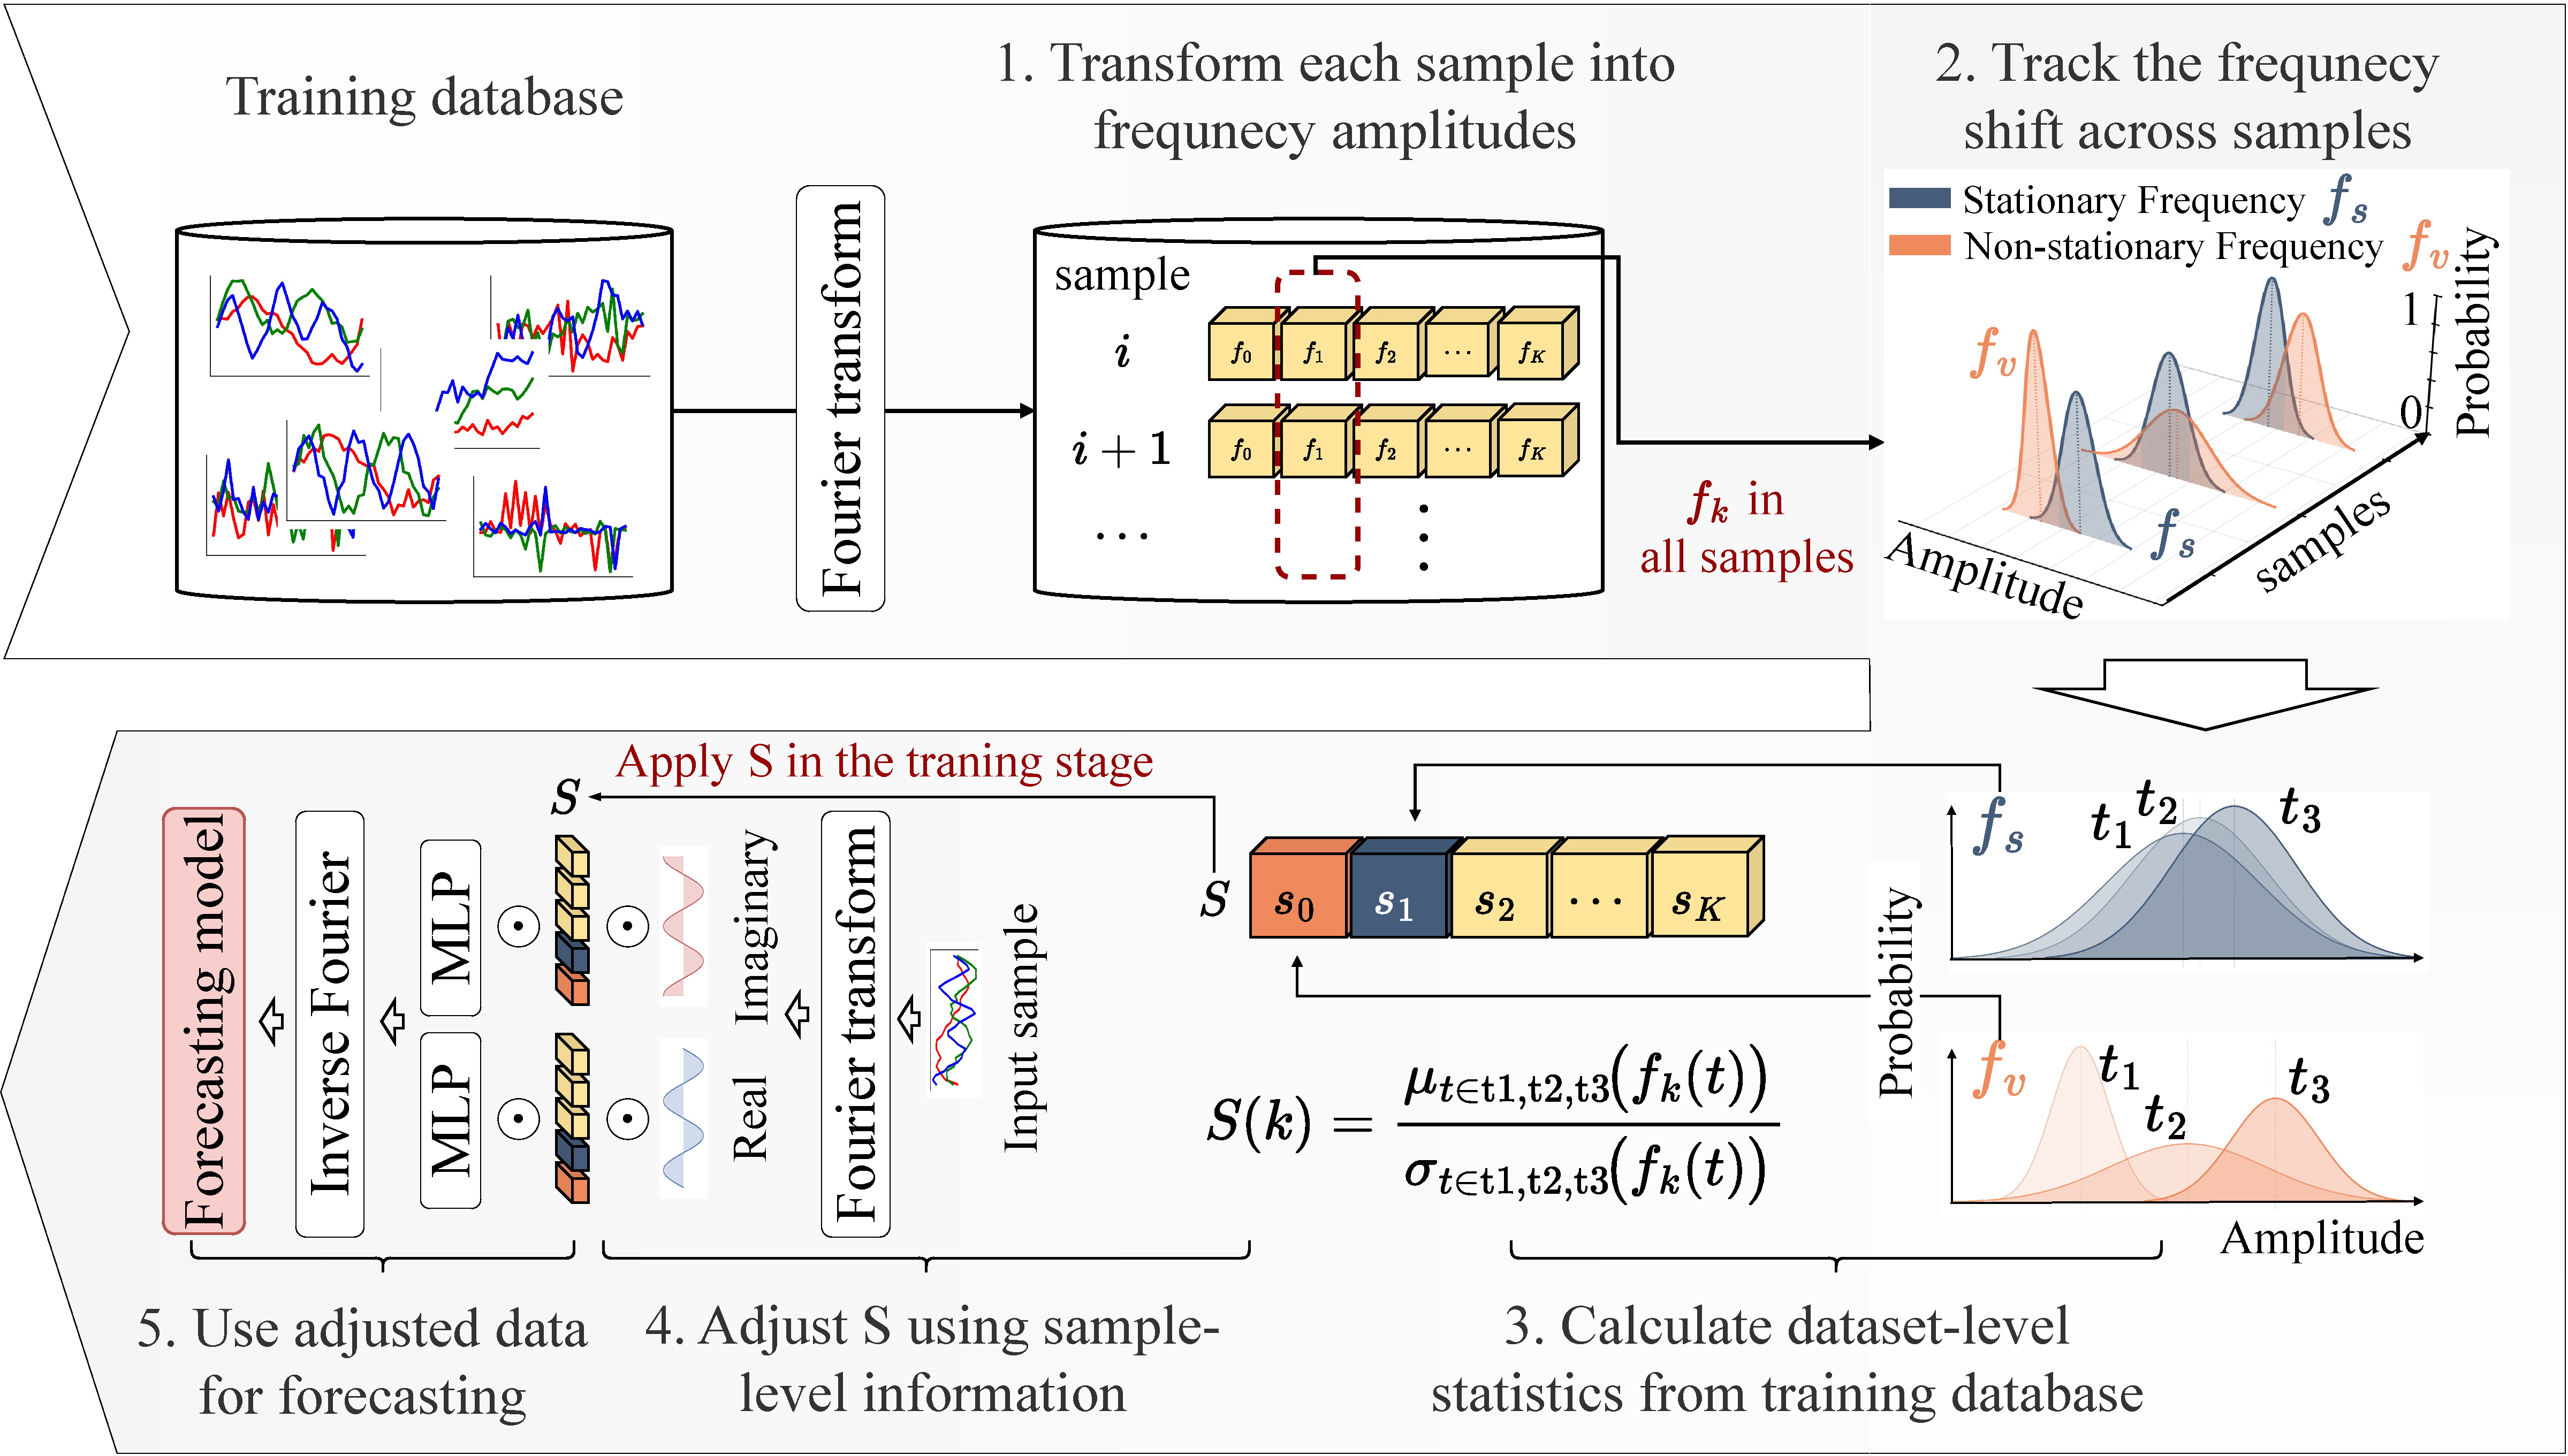
\includegraphics[width=0.83\linewidth]{pics/model.pdf}
  \caption{
    Overview of \method. 
    %Before training, we measure the stationarity for each frequency across the training set. %scores from the training set, and through MLPs, output weights for the real and imaginary DFT coefficients. 
    % During the training stage, each input time series is transformed into the frequency domain. Using these weights, we weight the frequencies. 
    % The weighted spectrum is then transformed into the time domain and serves as the input for the forecasting backbone model.
    \reviewhighlight{Before training, we first transfer all samples into the frequency domain and measure their cross-sample stationarity at the dataset level (steps 1 \& 2).}
    \reviewhighlight{These features are then used to learn frequency weights that measure frequency stationarity (step 3).}
    \reviewhighlight{During training, each input sample is transformed into the frequency domain and then weighted by the learned stationarity weights.}
    Finally, they are transformed to the time domain to serve as input to the forecasting models (steps 4 \& 5). 
    \method is optimized using the forecasting loss along with the backbone model.
  }
  \label{fig:model}
\end{figure*}



% \begin{wrapfigure}{r}{0.5\textwidth}
%     \centering
%     % \fbox{\rule{0pt}{1.5in} \rule{0.4\textwidth}{0pt}} % Placeholder box
%     %\vspace{-0.5cm}
%     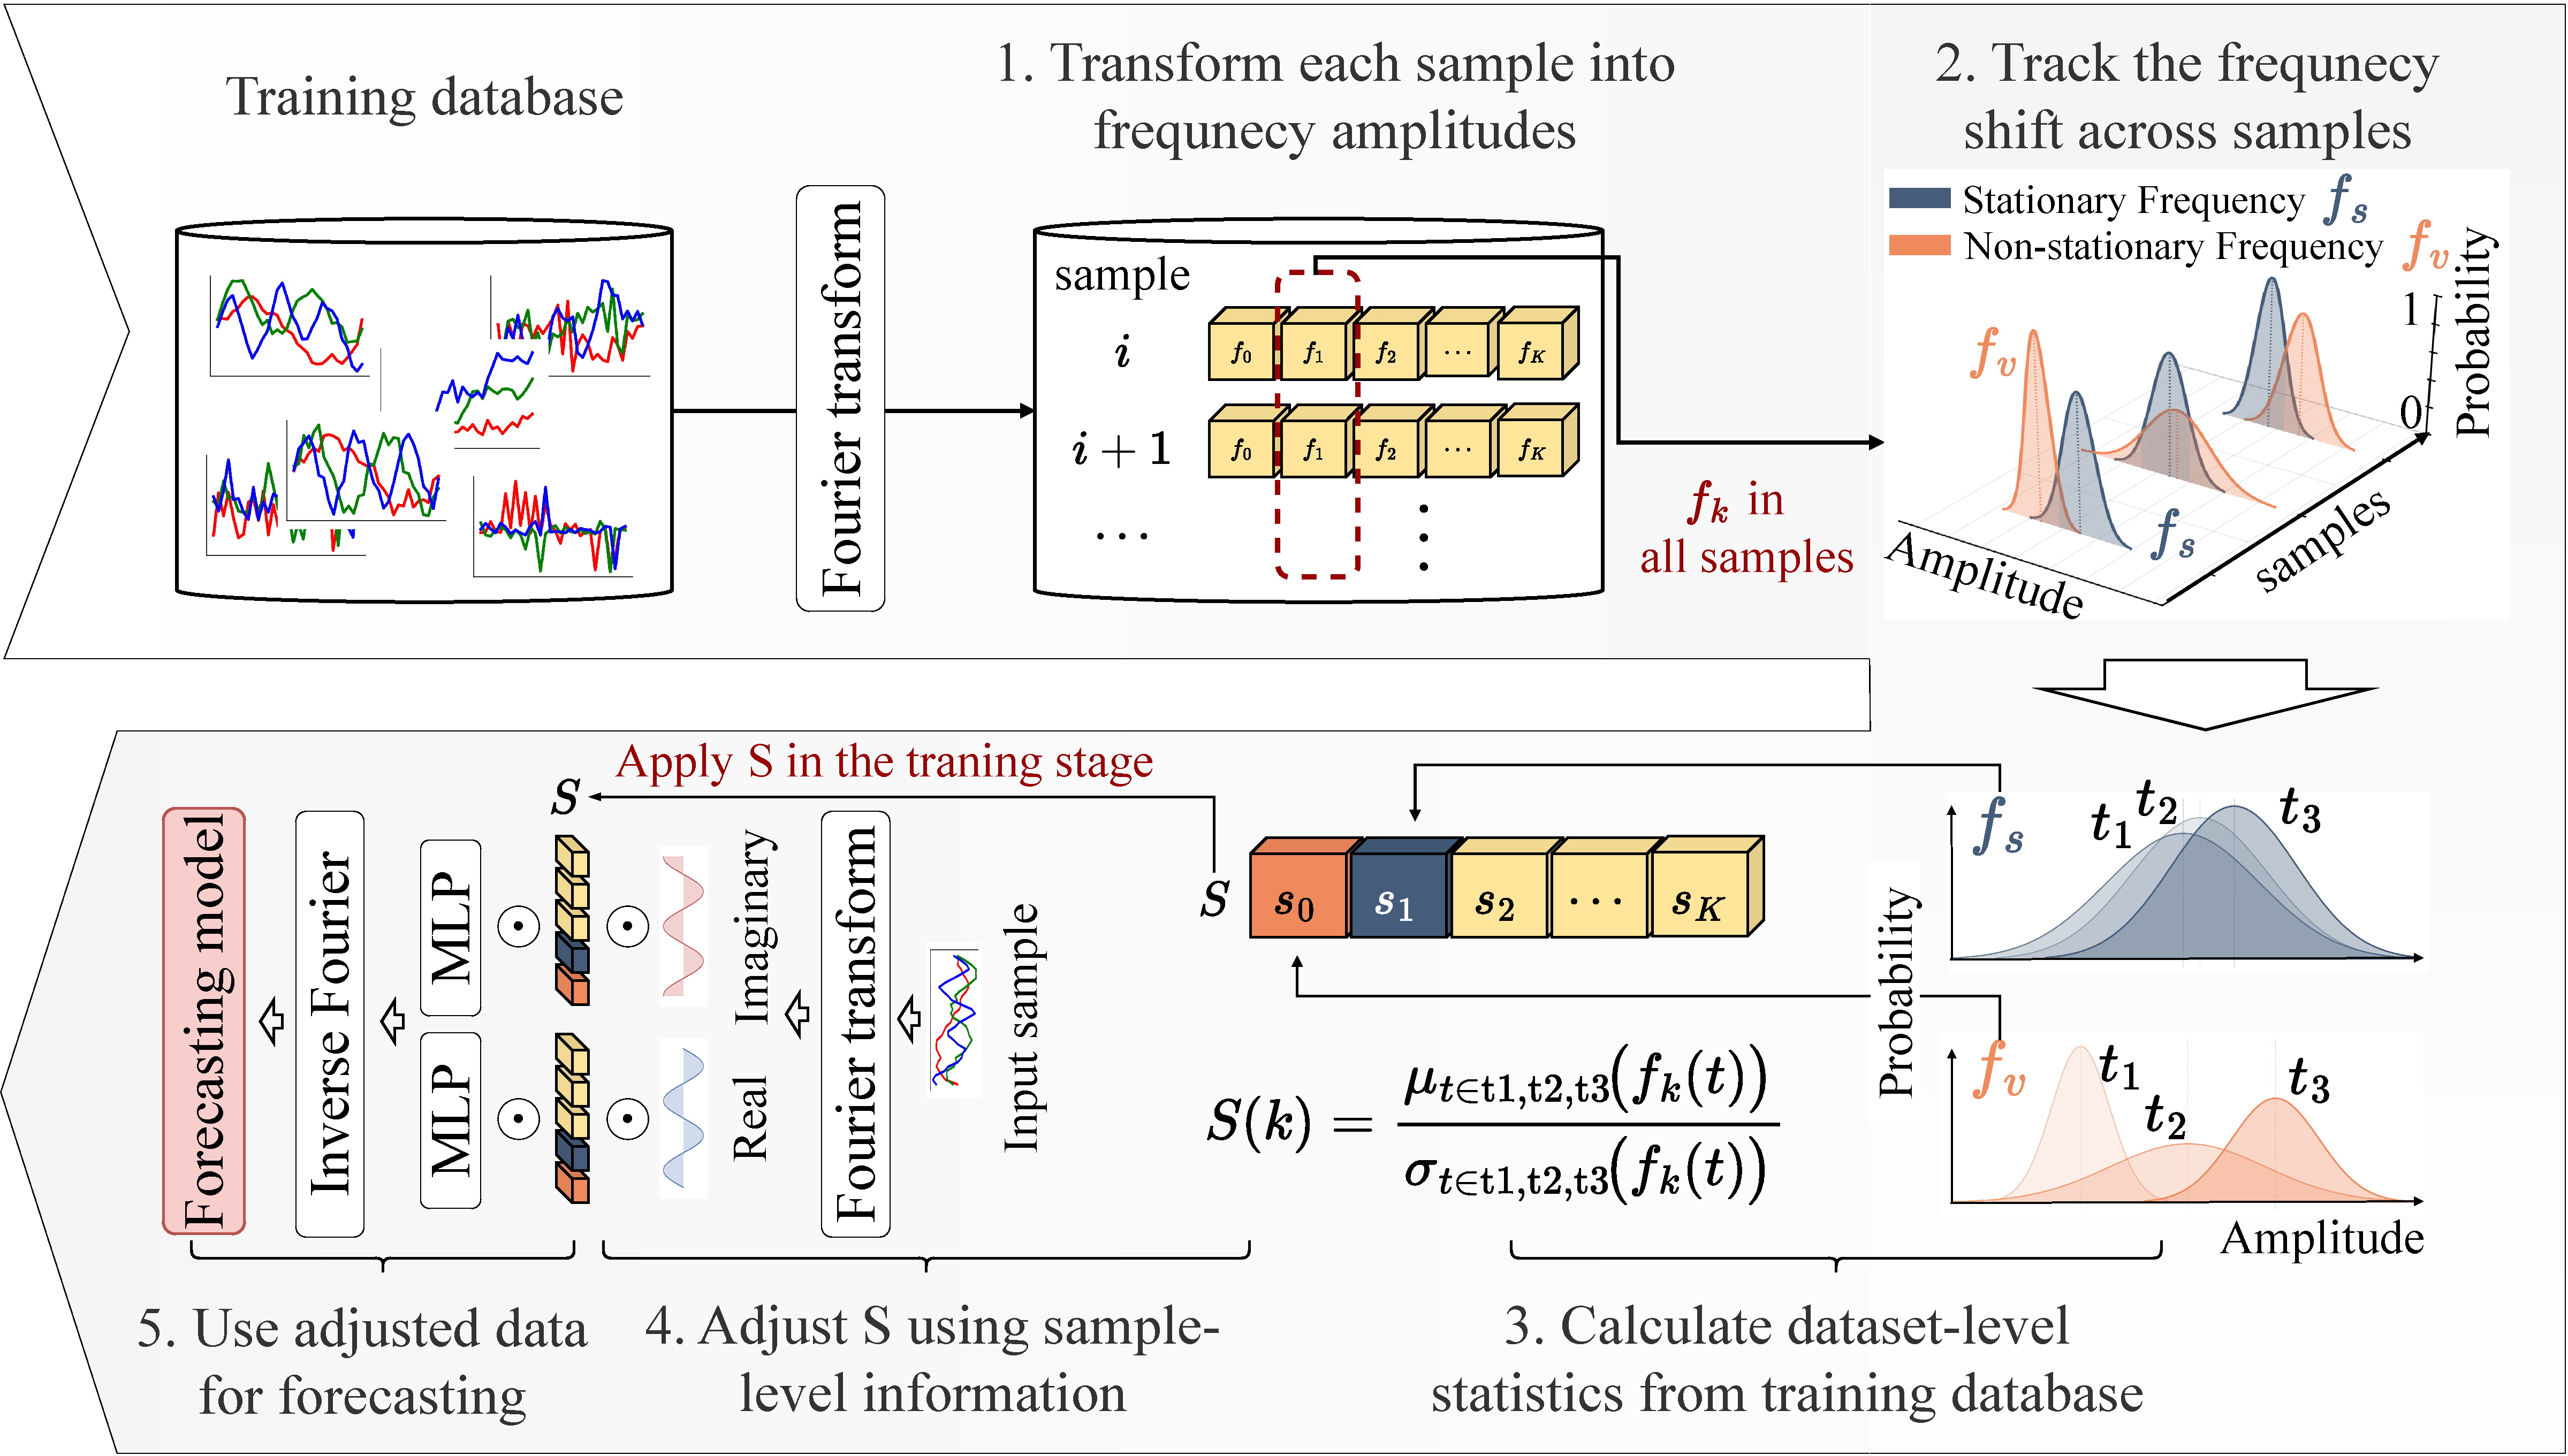
\includegraphics[width=0.5\textwidth]{pics/model.pdf}
%     % \vspace{-0.65cm}
%     \caption{Overview of \method. 
%     We first compute frequency-wise stationarity scores $S(k)$ from the training set, and through MLPs, output weights for the real and imaginary DFT coefficients. 
%     During the training stage, each input time series is transformed into the frequency domain, and the coefficients are multiplied by these weights to obtain the weighted spectrum. 
%     The weighted spectrum is then transformed to the time domain and serves as the input for the forecasting backbone model.
%     \method is optimized using the forecasting loss along with the backbone model.}
%     %\vspace{-0.2cm}
%     \label{fig:model}
% \end{wrapfigure}


\subsection{System Overview and FeedForward Pipeline}
\label{subsec:method-overview}

Figure~\ref{fig:model} shows the processing pipeline of \method.
It includes a two-stage modeling: 
%Our approach follows the problem definition in Section~\ref{sec:Preliminary Analysis}: we aim to identify frequency components that are stationary across samples. 
%To achieve this, we design 
(i) pre-training: measuring frequency stationarity in the entire training set; 
(ii) in-training: adaptively re-weighting frequency coefficients of each input sequence.

% \textbf{Stage 1: Dataset-level Stationarity learning. }
% For each sample $\mathbf{X}^{(i)} \in \mathbb{R}^{L \times C}$, we take the Discrete Fourier Transform (DFT) and obtain the amplitudes $A^{(i)}(k,c)$ for frequency $k$ and channel $c$.
% %For each sample $\mathbf{X}^{(i)}\!\in\!\mathbb{R}^{L\times C}$, we apply the Discrete Fourier Transform (DFT) to obtain frequency amplitudes, $A^{(i)}(k,c) \;=\;\big|\mathrm{DFT}\!\big(\mathbf{X}^{(i)}_{:,c}\big)_k\big|$.
% We aggregate across the training set to measure the stationarity of frequencies using $S(k,c)=\frac{\mu_{i\in\text{train}}\!\big(A^{(i)}(k,c)\big)}{\sigma_{i\in\text{train}}\!\big(A^{(i)}(k,c)\big)}$,
% % \begin{equation}
% % S(k,c)\;=\;\frac{\mu_{i\in\text{train}}\!\big(A^{(i)}(k,c)\big)}{\sigma_{i\in\text{train}}\!\big(A^{(i)}(k,c)\big)}.
% % \end{equation}
% where $\mu_{i\in\mathrm{train}}(\cdot)$ and $\sigma_{i\in\mathrm{train}}(\cdot)$ are the mean and standard deviation of the amplitude $A^{(i)}(k)$ for frequency $k$. 
% A larger $\mu$ indicates a higher energy proportion in the spectrum, while a greater $\sigma$ denotes higher sample dispersion.
% Thus, a higher $S(k)$ value indicates higher stationarity for frequency $k$.
% %$S$ aims to capture the distribution of each frequency component across the training set. 
% This allows our forecasting model to learn the overall stationarity of each component across different samples.
% % We do not assume that $S$ can fully capture the frequency stationarity.
% Here, $S$ is a reasonable way to summarize the observations of frequency $k$ across multiple samples.
% Through $S$, the model can access cross-sample variation information, while the MLPs in stage 2 can optimize the weights through training.
% %Meanwhile, $S$ is a dimensionless measure that allows for a fair comparison between different frequency components, thus avoiding uniform frequency scaling.

% \textbf{Stage 2. Sample-specific Learning \& Forecasting. }
% Given a sample $\mathbf{X}\in\mathbb{R}^{L\times C}$ we compute its DFT and obtain real and imaginary coefficients $\mathbf{R},\mathbf{I}\in\mathbb{R}^{K\times C}$. 
% Based on the pre-computed stationarity $\mathbf{S}\in\mathbb{R}^{K\times C}$, we use two independent MLPs to generate frequency weights:
% \begin{align}
% \mathbf{\lambda}_r=\mathrm{MLP}_r(\mathbf{S}),\quad 
% \mathbf{\lambda}_i=\mathrm{MLP}_i(\mathbf{S}). \label{eq:lambas}
% \end{align}
% The weighted coefficients are then obtained by element-wise multiplication:
% $
% \mathbf{R}_w=\mathbf{R}\odot\mathbf{\lambda}_r,\quad
% \mathbf{I}_w=\mathbf{I}\odot\mathbf{\lambda}_i.
% $
% We model real and imaginary parts separately to ensure that when the weighted coefficients are mapped to the time domain through inverse DFT, the resulting amplitudes remain non-negative and the inverse DFT produces valid real-valued sequences. 
% This stage acts as a lightweight frequency stationarity filter that enhances stationary components (high stationarity score) while suppressing non-stationary ones, addressing the distribution shift problem defined in Section~\ref{sec:Preliminary Analysis}.

% Finally, the reweighted coefficients $(\mathbf{R}_w,\mathbf{I}_w)$ are transformed to the time domain via inverse DFT 
% $
% \widetilde{\mathbf{X}}=\mathrm{iDFT}(\mathbf{R}_w+i\,\mathbf{I}_w),
% $
% and fed into the backbone forecasting models. 
% The whole framework is optimized end-to-end using the forecasting MSE loss. 

\noindent\textbf{Stage-I: Dataset-level Stationarity Learning}
\begin{itemize}[leftmargin=1.5em]
    \item \emph{Step 1.} \reviewhighlight{For each sample $\mathbf{X}^{(i)} \in \mathbb{R}^{L \times C}$ from a multi-channel time series training dataset $\mathcal{X} = \{\mathbf{X}^{(i)}\}_{i=1}^N$, we take the Discrete Fourier Transform (DFT) and obtain the amplitudes $\mathbf{A}^{(i)}(k,c)$ for frequency $k$ and channel $c$. Where $L$ represents the length of each sample, C is the number of channels, and $K$ is the number of frequency components.}
    \item \emph{Step 2.} We aggregate across the training set to measure the stationarity of frequencies using
    %\begin{equation}
    $$\color{red}\mathbf{S}(k,c)\;=\;\frac{\mu_{i\in\text{train}}\!\big(\mathbf{A}^{(i)}(k,c)\big)}{\sigma_{i\in\text{train}}\!\big(\mathbf{A}^{(i)}(k,c)\big)}$$,
    %\end{equation}
    where $\mu_{i\in\mathrm{train}}(\cdot)$ and $\sigma_{i\in\mathrm{train}}(\cdot)$ are the mean and standard deviation of the amplitude $\mathbf{A}^{(i)}(k,c)$ in all samples. 
    A larger $\mu$ means a higher energy proportion, while a greater $\sigma$ denotes higher sample dispersion. 
    \reviewhighlight{Thus, a higher $\mathbf{S}(k,c)$ reflects more stationary frequency behavior.}
    \item \emph{Step 3.} In this step, we save the calculated $\mathbf{S}$ from Step 2 and pass it to the forecasting model.
    Through $\mathbf{S}$, the model can access cross-sample variation information, while the MLPs in Stage~II can further optimize the weights through training.
    This aims to allow the forecasting model to learn the overall stationarity of each component across the dataset, 
    %capture the distribution of each frequency component across the training set 
    and use this information to learn a stationary representation of data during the training.
    %This 
    %Here, $S$ is a reasonable way to summarize the observations of frequency $k$ across multiple samples. 
\end{itemize}

\noindent\textbf{Stage-II: Sample-specific Learning \& Forecasting}
\begin{itemize}[leftmargin=1.5em]
    \item \emph{Step 4.} In the training stage, given an input sample $\mathbf{X}\in\mathbb{R}^{L\times C}$, we compute its DFT and obtain real and imaginary coefficients $\mathbf{R},\mathbf{I}\in\mathbb{R}^{K\times C}$. 
    \reviewhighlight{Based on the pre-computed stationarity $\mathbf{S}\in\mathbb{R}^{K\times C}$, we use two independent MLPs to generate frequency weights:}
    \begin{align}
    \color{red}\mathbf{\lambda}_r=\mathrm{MLP}_r(\mathbf{S}),\quad
    \mathbf{\lambda}_i=\mathrm{MLP}_i(\mathbf{S}). \label{eq:lambas}
    \end{align}
    The weighted coefficients are then obtained by element-wise multiplication:
    $\mathbf{R}_w=\mathbf{R}\odot\mathbf{\lambda}_r,\quad
    \mathbf{I}_w=\mathbf{I}\odot\mathbf{\lambda}_i.$
    We model the real and imaginary parts separately to ensure that when the weighted coefficients are mapped to the time domain through the inverse DFT, the resulting amplitudes remain non-negative, allowing the inverse DFT to output real-valued sequences. 
    \reviewhighlight{In this stage, \method serves as a lightweight frequency stationarity filter, enhancing stationary components (those with a high stationarity score) while suppressing non-stationary ones, thereby addressing the distribution shift problem defined in Section~\ref{sec:Preliminary Analysis}.}
    \item \emph{Step 5.} Finally, the weighted coefficients $(\mathbf{R}_w,\mathbf{I}_w)$ are transformed to the time domain via inverse DFT 
    $\widetilde{\mathbf{X}}=\mathrm{iDFT}(\mathbf{R}_w+i\,\mathbf{I}_w)$,
    and fed into the backbone forecasting models. 
    $\widetilde{\mathbf{X}}\in\mathbb{R}^{H\times C}$ is the final output of \method and the input of the backbone model, where $H$ denotes the forecasting horizon.
    The whole framework is optimized end-to-end using the forecasting MSE loss.  
\end{itemize}



%In the following subsections, we will connect this weighting mechanism to Bochner’s and Mercer’s theorems, showing that learning frequency-wise weights can be understood as learning stationary representations in a principled way.

%\newpage

%\subsection{Model Design and Training}

% {\color{blue}
% (Lingwei: I think we should make our proposed method very clear, maybe by starting with a description of our pipelin from input data to transformed input to final output (for what purpose?) $\lambda$.
% At this point, we should just say $\lambda$ are weights rather than assigning special meanings like "eigenvalues".
% We can then in the subsequent sections say that these empirical-looking weights are actually motivated by deep math!
% To do this, we should consider removing redundant notations like ReLU or weight/bias matrices to make it simple to emphasize our unique things.)
% }

% Learning the eigenvalues $\lambda$ is equivalent to learning the weights applied to basis functions to represent signal waves.
% Algorithm \ref{alg:alg1} lists our algorithm that uses procedures in Alg. \ref{alg:compute_scores} and \ref{alg:apply_weights}.
% Specifically, we can have two MLPs to learn the coefficients to be multiplied to the Fourier basis:
% \begin{align}
%    &\hat{\lambda}_{2j} 
% =\mathbf{W}_{2}^\mathrm{(cos)} \,\text{ReLU}\bigl(\mathbf{W}_1^\mathrm{(cos)}\,s_{2j} + \mathbf{b}_1^\mathrm{(cos)}\bigr)
%    + \mathbf{b}_2^\mathrm{(cos)}, \nonumber\\
%   &\hat{\lambda}_{2j+1} 
% =\mathbf{W}_{2}^\mathrm{(sin)} \,\text{ReLU}\bigl(\mathbf{W}_1^\mathrm{(sin)}\,s_{2j+1} + \mathbf{b}_1^\mathrm{(sin)}\bigr)
%    + \mathbf{b}_2^\mathrm{(sin)}.
%    \label{eq:eigenvalues}
% \end{align}
% %$s:=\frac{\hat\mu}{\hat\sigma}$
% where $\mathbf{W}, \mathbf{b}$ are learnable weights and bias for even and odd numbers of eigenvalues {\color{black}(i.e., the real and imaginary parts of the Fourier coefficients)}.
% $s$ is an estimated statistic, dividing the mean by the standard deviation \citep{abdi2010coefficient3}.
% %is a heuristic starting point to guide learning.
% % It captures the distribution of each frequency component across the entire training set. 
% % This allows the forecasting model to learn the \textit{overall stability} of each component across different samples.
% % $S$ is a dimensionless measure that allows for a fair comparison between different frequency components, thus avoiding uniform frequency scaling.
% It captures the distribution of each frequency component across the entire training set. 
% This allows the forecasting model to learn the overall stability of each component across different datasets.
% Moreover, $s$ is a dimensionless measure allowing a fair comparison between different frequency components.
% During the training phase,\method first computes $s$ from the entire training set and saves it, as shown in Algorithm~\ref{alg:compute_scores}. 

% % Notably, $s$ is a dimensionless metric that fairly compares the temporal fluctuations of variables from different distributions, so it can help us prevent frequencies with larger mean amplitudes from dominating.
% %These make $s$ a good starting point for the MLP.

% % \begin{itemize}[left=0pt]
% %     \item It captures the distribution of each frequency component across the entire training set. 
% %     This allows the forecasting model to learn the \textit{overall stability} of each component across different samples.
% %     \item $S$ is a dimensionless measure that allows for a fair comparison between different frequency components, thus avoiding uniform frequency scaling.
% % \end{itemize}



% Then we apply the learning weights, i.e., $\lambda$, to the input real and imaginary parts of the transformed data.
% % we first transform the inputs into the frequency domain and gain the real and imaginary parts of the transformed data.
% %Therefore, 
% Then, the feature representation is constructed by:
% \begin{align}
%  \widehat{\Phi}^\text{even}_t(\omega) =  \cos\left(\frac{2\pi j \omega}{t}\right) \odot \hat{\lambda}_{2j}, 
%  \quad
%   \widehat{\Phi}^\text{odd}_t(\omega)  =  \sin \left(\frac{ 2\pi j \omega}{t} \right) \odot \hat{\lambda}_{2j+1},
%   \label{eq:eigenfunctions}
% \end{align}

% The MLPs should be capable of finding Fourier coefficients that correspond to a suitable kernel to represent the frequency components of the input time series. 
% %When this is achieved, we transform the representations back to the time domain for downstream tasks.
% As shown in the Algorithm~\ref{alg:apply_weights}, we transform the learned representations into the time domain via inverse Fourier transforms.
% Finally, we feed them into forecasting models, following a similar strategy to normalization methods \citep{kim2021RevIN, fan2023dish, han2024sin, liu2023SAN, ye2024FAN}.

% During the test phase, \method uses the saved $s$ from the training set and the frozen MLPs, yielding processed inputs for the trained forecasting model.
% \method requires no extra training stages or loss functions and can be trained jointly with the forecasting model.

%Overall, in the training phase, (i) \method first computes the starting point $s$ from the entire training set and saves it, as shown in Algorithm~\ref{alg:compute_scores}. 
%(ii) \method then takes the raw data and the precomputed $s$ as inputs: $s$ is fed into two independent MLPs to learn real and imaginary weight vectors $\lambda$ (shown in Eq~\ref{eq:eigenvalues}), which are applied via Hadamard multiplication to real and imaginary part of the input data (Eq~\ref{eq:eigenfunctions} and Algorithm~\ref{alg:apply_weights}). 
%\method requires no extra training stages or loss functions and can be trained jointly with the forecasting model.
%In the test phase, \method uses the saved $s$ from the training set and the frozen MLPs, yielding processed inputs for the trained forecasting model.
% {\color{red}

% Representation learning. After learning, what should we do? 
% You can specifically focus on Alg. \ref{alg:apply_weights} to explain what is np.fft.rfft, and how the returned thing is used in later predictions and inference.
% }


% \lstdefinestyle{pycode}{
%   language   = Python,
%   basicstyle = \ttfamily\footnotesize,
%   keywordstyle=\color{Plum},
%   commentstyle=\color{PineGreen},
%   stringstyle =\color{orange},
%   showstringspaces=false,
%   columns    = fullflexible,
%   tabsize    = 4,
%   mathescape = true,
%   escapeinside={(*@}{@*)}
% }

% \begin{figure}[t]
%   \centering
%   % -------------------- Left block ---------------------------------
%   \begin{minipage}[t]{0.49\textwidth}
%     \begin{algorithm}[H]
%       \caption{Compute Starting Point $s_j$}\label{alg:compute_scores}
%       \lstset{style=pycode,caption={}}
% \begin{lstlisting}
% def compute_stability_scores(X):
%     """
%     X: (N, T) the train set
%     """
%     amp  = np.abs(np.fft.fft(X, axis=1)) 
%     # per-freq mean & std for each $\omega_j$
%     mean = amp.mean(axis=0)    
%     std  = amp.std(axis=0) + 1e-5            
%     return mean / std                        # Compute $s_j$
% \end{lstlisting}
%     \end{algorithm}
%   \end{minipage}\hfill
%   % -------------------- Right block --------------------------------
%   \begin{minipage}[t]{0.49\textwidth}
%     \begin{algorithm}[H]
%       \caption{Apply Fourier Coefficients $\lambda_j$}\label{alg:apply_weights}
%       \lstset{style=pycode,caption={}}
% \begin{lstlisting}
% def weight_spectra(x, s, f_cos, f_sin):
%     """ 
%     f_*: MLP layers
%     """
%     X = np.fft.fft(x)                      
%     X[0::2] *= f_cos(s[0::2])               
%     X[1::2] *= f_sin(s[1::2])              
%     # transform back to the time domain
%     return np.fft.ifft(X, n=len(x))        
% \end{lstlisting}
%     \end{algorithm}
%   \end{minipage}
% \end{figure} 


% Temporal distribution shifts pose a fundamental challenge for time-series forecasting. There are two scenarios of distribution shifts. When the distribution shifts only occur
% between the training and test domains, meta learning and transfer learning approaches have been developed. The other scenario is much more challenging:
% distribution shifts occurring continuously over time \citep{wang2023koopman}.

% Time-series forecasting models often suffer badly from a unique characteristic in time-series data:
% their statistical properties, e.g., mean and variance, can change over time. 
% This nonstationarity of statistical properties is known as the distribution shift problem, and it can incur mismatch between the data on which the model is trained and that the model is deployed, leading to performance degradation when they do not have a significant overlap \citep{kim2021RevIN}.


% Some recent research found that if we remove the non-stationary information from the input series, e.g. by removing the time-dependence of mean and standard deviation from the input instances, the mismatch in the distributions can be reduced, thereby improving model performance. 
% This idea justifies recent discoveries that normalize the input sequences with a $z$-score to help model learning and denormalize the model output to recover time dependency.
% They balance uniformity and variability, removing distributional discrepancies while preserving inherent fluctuations in time series, thereby enhancing generalization.
% Such methods ensure the forecasting results are accurate (by normalization) while maintaining the inherent variability and fluctuation in the time series (by denormalization), enhancing generalization.
% Since two operations are applied only to the inputs and outputs of models, these methods function as ``model-friendly modules'' that could be easily integrated into various forecasting models without any transformation.

% While the normalize-denormalize methods have shown some promise by aligning the training/test set distributions, they do not satisfactorily address the issue that the model itself may have difficulty in discerning complex input sequences as a composition of waves that the model needs to distinguish  \citep{Digital_Signal_Processing, he2023raincoat, Timesnet, Piao2024fredformer}.
% Indeed, if we view a time series sample as an instantiation of some zero-mean stochastic process $\{X_t\}$, then its frequency characteristics can be obtained from its spectral representation \citep{adak1998time-dependent}:
% \begin{align}
%     X_t = \int A(\omega) e^{i2\pi \omega t  }\, \mathrm{d} p(\omega),
%     \label{eq:adak}
% \end{align}
% where $\omega$ denotes the frequency component and $A$ is the amplitude function.
% Eq. \ref{eq:adak} states that there is correspondence between variability in the time domain and amplitude in the frequency domain. 
% Therefore, the temporal distribution shift problem can be avoided as a whole if we can find a good representation of $\omega$ encoding common frequency characteristics in both training and test datasets. 
% Eq.(\ref{eq:adak}) suggests a viable way to tackling distributional shift: 

% Our key idea lies in that  even $x_\text{train} \sim p(x|t_\text{train})$ and $x_\text{test} \sim p(x|t_\text{test})$ may differ significantly, their underlying frequency components $\omega_\text{train}, \, \omega_\text{test}$ may be well-represented by a same shift-aware representation.
% We tackle distributional shift by learning this representation.
% distributions $p(\omega_\text{train})$ and $p(\omega_\text{test})$ could still be similar.
% Under this assumption, learning a good representation of training frequency $\psi(\omega_\text{train})$ helps in representing test patterns as well, which eventually addresses the distributional shift problem.



\subsection{Theoretical Analysis}\label{sec:Theoretical Analysis}


\reviewhighlight{Our frequency weighting in the previous section is the result of the following theoretical analysis.}
\reviewhighlight{This section connecting nonstationarity to spectrum analysis is novel to the best of our knowledge.}



\noindent\textbf{Existence of Time-Averaged Representation.}
% \subsection{Fourier Transform Implicitly Induces Frequency Representation}\label{sec:bochner}
% Specifically, we are interested in distinguishing between the frequency components that contribute most to the variability.
% This can be done, e.g. by capturing the frequency component-wise difference $\omega_1 - \omega_2$.
% Inspired by the connection between nonstationary processes and time series data in Eq.(\ref{eq:adak}),
% our goal is to learn a representation function $\psi$ such that of frequency components from both training and test datasets can be well represented.
% We show that by such distributional-shift-aware representations can be learned as a result of integrating over all time variables, by a classic result from harmonics analysis about Fourier transform mapping time series to the frequency space \citep{berg84harmonic}.
% Our objective is to learn a representation function $ \psi $ that captures frequency components in a way that is invariant to distributional shifts between training and test datasets. 
{\color{black}
\reviewhighlight{We connect the learning of frequency weights Eq.(\ref{eq:lambas}) to spectrum analysis by noticing that these weights correspond eigenvalues that characterize frequency space representations that discern frequency components responsible for distributional shifts.}
We begin our analysis with the assumption:
% To begin with the analysis,  we revisit the following basic result.
% view of distributional shift in time series.
% However, in this paper, we aim to provide a more principled method that considers all possible time conditions via $p(x) = \int p(t) p(x|t) \mathrm{d}t$.
% To this end, we adopt a nonstationary stochastic process view of distributional shift in time series.
% \textbf{Time series as a non-stationary process.}
% Real-world time series data is a discrete-time signal $X$, which is usually considered a nonstationary process. 
% A stochastic process is nonstationary if its statistical properties change over time \citep{hammond1996analysis_of_nonstationary, Non-stationary, salles2019nonstationary_methods}. 
% The nonstationary process view allows us to characterize the time series data via its frequency spectra. 
% While the normalize-denormalize methods have shown some promise by aligning the training/test set distributions, they do not satisfactorily address the issue that the model itself may have difficulty in discerning complex input sequences as a composition of waves that the model needs to distinguish  \citep{Digital_Signal_Processing, he2023raincoat, Timesnet, Piao2024fredformer}.
% Without loss of generality, we assume a timeseries sample is an instantiation of some zero-mean stochastic process $\{x_t\}$.
% Its frequency characteristics can be obtained from its spectral representation \citep{adak1998time-dependent}:
% \begin{align}
%     \mathbf{X}_t = \int A(\omega) e^{2\pi i  \omega t  }\, \mathrm{d} p(\omega),
%     \label{eq:adak}
% \end{align}
% where $\omega$ denotes the frequency component and $A$ is the amplitude function.
% Eq. (\ref{eq:adak}) states that time-sequential data can be derived from the integration of harmonic waves \citep{Xue2023-cosnet}.
% One might wonder whether such an integration exists for the time domain so that a frequency representation as an average over all time variations exists.
% We show that there is indeed such a representation in Theorem \ref{thm:bochner}.
% But before that we need to formally make an assumption on the dataset.
% Eq. (\ref{eq:adak}) is reminiscent of Fourier transform. 
% In fact, it is a classic result that 
}



% Our goal is to learn a representation function $\psi$ that captures shift-invariant frequency components shared between training and test data.
% We achieve this by classic harmonics analysis results about Fourier transform \citep{berg84harmonic}.
% Specifically, we aim to learn a representation function $\psi$ in the frequency space that 
% Therefore,  the problem is cast under the representation learning  framework where the goal is to learn a function $\psi$ such that $\psi(\omega_1 - \omega_2)$ can give the model sufficient information to separate the two frequency components.
% We achieve this by leveraging classic tools from harmonic analysis \citep{berg84harmonic} to learn an orthonormal basis in the frequency space to represent the input sequences.
% Formally, let frequency components be in the range $F= [0, \omega_\text{max}]$.
% We define a positive semi-definite kernel by $k : F\times F \rightarrow \mathbb{R}$ \citep{Scholkopf-kernel}. 
% Given two frequency components $\omega_1, \omega_2$, we have $k(\omega_1, \omega_2) = \innerProduct{\Phi(\omega_1)}{\Phi(\omega_2)} = \psi(\omega_1 - \omega_2)$ with some  $\psi : [0, \omega_\text{max}] \rightarrow \mathbb{R}$.
% $\Phi$ is the feature representation that defines how the frequency components are embedded into high dimensional spaces.
% We begin with our assumption on the data.
% We begin our proposed method by elaborating on how the Fourier transform acting upon time series data implicitly induces a valid kernel.

% {\color{red}
% Fourier transform on top of $x$ gives $\omega$.  
% Let us assume that train and test data share similar frequency component distributions.
% So the training dataset can be seen as first drawing $t \sim p(t)$, then $x \sim p(x|t)$.
% Let us assume that the datasets is formed by drawing multiple times each with its own procedure.
% Applying Fourier transform on this dataset is
%  \texttt{FourierTransform}($x$) = $\int_{\mathbb{R}}e^{i t\omega}p(x|t) p(t) \mathrm{d}t = \int_{\mathbb{R}}e^{i t\omega} p(\omega) p(t) \mathrm{d}t$.
% }

\begin{assumption}\label{thm:assumption}
    \reviewhighlight{The time series dataset $\mathcal{X} = \{\mathbf{X}^{(i)}\}_{i=1}^N$ is composed of multiple samples from $t_i \sim p(t)$ and $x^{(i)} \sim p(x | t_i)$ so it can sufficiently representation the distributions.}
\end{assumption}
% Given 
\reviewhighlight{We assume that the time series dataset can sufficiently represent the time variations.}
\reviewhighlight{This assumption is realistic in many real-world datasets such as electricity or stock markets that collect data on many-year-basis.}
These datasets compose a challenge to normalization methods, since removing empirical estimates $\bar{\mu}, \bar{\sigma}$ from a batch does not equal removing $\mu_{t_i}, \sigma_{t_i}$ that is governed by a specific $t_i$.
It is intractable to identify which data batch is governed by a unique time structure.
Our method instead turns to \emph{a time-averaged representation}.
\reviewhighlight{We integrate over time by applying Fourier transform on data.}
The next theorem formalizes this idea.


% As a result, applying Fourier transform on $\mathcal{X}$ can be considered as applying on the distributions $p(t)p(x|t)$. 
% Given this assumption, we state the next theorem that connects Fourier transform of time series data to kernel functions in the frequency space.


\begin{myTheo} [Bochner's Theorem \citep{Scholkopf-kernel}]\label{thm:bochner}
A kernel function $k(x, y) \geq 0$ is a distance measure of input $x, y$.
It is valid if and only if there exists a probability density that is the Fourier transform of the kernel.
\end{myTheo}
\reviewhighlight{The fact that we assume data is generated by $t_i \sim p(t),\,x^{(i)} \sim p(x | t_i)$ plus we apply Fourier transform to $\mathcal{X}$ imply that a kernel function exists on the frequency domain:}
% Let us recall the time distribution $p(t)$ defines how the time dynamics change and affects the data distribution.
% Then Bochner's theorem tells us by applying the Fourier transform on the input time series necessarily induce a kernel $k$ in the frequency domain:
\begin{align}
\label{eqn:bochner}
\begin{split}
    % & k(\omega_1, \omega_2)|_x  = \int_{\mathbb{R}}e^{i t(\omega_1 - \omega_2)}p(t) p(x|t) \mathrm{d}t = \expectation{t}{e^{i t(\omega_1 - \omega_2)}}\bigg|_x.
    k(\omega_1, \omega_2)|_x  = \int_{\mathbb{R}}e^{i t(\omega_1 - \omega_2)} \mathcal{X} \mathrm{d}t = \expectation{t}{e^{i t(\omega_1 - \omega_2)}}\bigg|_x.
    % & k(\omega_1, \omega_2 | x) = \psi(\omega_1 - \omega_2 | x) = \int_{\mathbb{R}}e^{i t(\omega_1 - \omega_2)}p(x,t) \mathrm{d}t = \expectation{t}{e^{i t(\omega_1 - \omega_2)}} 
    \end{split}
\end{align}
where we use $|_x$ to denote the dependency on $x$. 
\reviewhighlight{While in practice the dataset $\mathcal{X}$ needs to be infinitely large to sufficiently represent the distributions, we can expect that with a reasonably sized dataset that comprises multiple samples of $t$, the existence of a kernel is guaranteed.}
\reviewhighlight{As the result of integration over time, it is also reasonable to expect that the kernel as a time-averaged representation should perform better than the normalization methods.}
% For uncluttered notations, we drop it in the following sections.
% The kernel is {implicitly} induced as a result of Fourier transform on nonstationary data.
% While $p(t)$ describes how $t$ changes, it is intractable to quantify the distributional shift, since the data are only sampled at finite times.
% Nonetheless, the implicit kernel representation already integrates out the time variable and hence depends only on frequency.

% {\color{blue}
% (\textbf{Lingwei: I am considering removing this part that is not directly related to our proposal to simplify things.
% This can for example merge section 3.3 into 3.2)}

% To learn the kernel representation, we define $\phi_{t}(\omega) := e^{i\omega t}$. 
% By the Euler's formula and the fact that the kernel function $k$ is real, we arrive at:
% \begin{align}
%     \begin{split}
%         k(\omega_1,\omega_2) = \expectation{t}{\phi_{t}(\omega_1) \phi^*_{t}(\omega_2) } = \expectation{t}{\cos(t (\omega_1 - \omega_2))}.
%     \end{split}
% \end{align}
% It is a classic result in kernel methods to approximate the kernel with Monte-Carlo samples \citep{rahimi-RKS,Yu2016-orthogonalRKS}.
% Specifically, this is done by drawing $d$ samples $t_1, \dots t_d \sim p(t)$ to construct finite dimensional feature representations:
% \begin{align*}
%     \widehat{\Phi}_t(\omega) &= \frac{1}{\sqrt{2d}}\left[\cos(t_1 \omega), \sin(t_1 \omega) , \dots, \cos(t_d \omega), \sin(t_d \omega)\right] \in \mathbb{R}^{2d}, \\
%     \innerProduct{\widehat{\Phi}_t(\omega_1)}{\widehat{\Phi}^{*}_{t}(\omega_2)} &= \frac{1}{2d}\sum_{i=1}^{d} \cos (t_i \omega_1) \cos(t_i \omega_2) + \sin(t_i \omega_1) \sin(t_i \omega_2)\\
%     &\approx \expectation{t}{\cos(t (\omega_1 - \omega_2))}.
% \end{align*}
% % $\widehat{\Phi}_t(\omega) = \frac{1}{\sqrt{d}}\left[\cos(t_1 \omega), \sin(t_1 \omega) , \dots, \cos(t_d \omega), \sin(t_d, \omega)\right]$ such that $\innerProduct{\widehat{\Phi}_t(\omega_1)}{\widehat{\Phi}^{*}_{t}(\omega_1)} = \frac{1}{d}\sum_{i=1}^{d} \cos (t_i \omega_1) \cos(t_i \omega_2) + \sin(t_i \omega_1) \sin(t_i \omega_2)$
% % and the fact that the kernel is real, the expectation can be written as $k(\omega_1,\omega_2) = E_{t}\big[\cos(t (\omega_1 - \omega_2))\big]$.
% % It is a classic result in the kernel methods to approximate the expectation .
% % Since the kernel $k$ and the probability measure $p(\omega)$ are real, we only take the real part of (\ref{eqn:bochner}) and arrive at:
% % \begin{equation}
% %     k(\omega_1,\omega_2) = E_{t}\big[\cos(t (\omega_1 - \omega_2))\big]=E_{t}\big[\cos(t\omega_1)\cos(t \omega_2) + \sin(t\omega_1)\sin(t \omega_2)\big].
% % \end{equation}
% For example, if we assume the kernel is an RBF kernel, then the corresponding distribution $p(t)$ is a Gaussian distribution \citep{rahimi-RKS}.
% However, this assumption may be too restrictive and one can choose instead to learn $p(t)$.
% \citet{Xu2019-attention-time-bochner} proposed to learn the sampling distribution for time embeddings in the attention architecture.
% But doing necessitates the test data to help quantify the temporal distribution shift, which is not desirable in many circumstances.
% }

% \subsection{Learning Explicit Orthonormal Frequency Basis for Implicit Representation}\label{sec:mercer}







\noindent\textbf{Adapting Time-Averaged Representation to Data.}
{\color{black}
\reviewhighlight{The kernel function in Eq. (\ref{eqn:bochner}) is implicit since we know it exists but have no access to it.}
\reviewhighlight{To exert the kernel as a distance measure, we can adapt it to input data so the distances between important and unimportant frequency components are emphasized most.}
\reviewhighlight{To this end, we explicitly learn the kernel based on the Mercer's theorem.}
% As involving test data in the training procedure is not desired, we study learning  representations that are invariant to both the training and test data.
% % Instead, we can leverage the properties of kernel function to find good representations of frequency components.
% Fortunately, this is possible by the following theorem that connects the induced kernel to orthonormal basis in the frequency space.
% Orthonormality nature is the optimal representation in the frequency space \citep{ninness1996orthonormal_1,wahlberg1991_orthonormal_2} and hence no further adaptation of learned representation to the test data is needed.
% To this end, we introduce the next theorem which connects the induced kernel to orthonormal basis in the frequency space.
% {\color{red}
% %为什么要分解/正交？
% What is big deal about orthonormal basis? It is the best representation one can find?}
% \{\citep{ wahlberg1991_orthonormal_2, van1995_orthonormal_5, ninness1996orthonormal_1, ninness1999_orthonormal_4, wahlberg2002_orthonormal_3}\}

\begin{myTheo}[Mercer's Theorem \citep{mercer1909mercer}]\label{thm:mercer}
% Assume that (1) $\sum_{i,j=1}^N c_i c_j k(x_i, y_j) > 0 $ for any set of points $\{c_i\}_{i=1}^N, \{x_i\}_{i=1}^N$;
% (2) $\int_{\mathcal{X}}\int_{\mathcal{X}} k^2(x,z) \mathrm{d}p(x)\mathrm{d}p(z) < \infty$.
A valid, positive definite kernel function can be represented
by a set of eigenfunctions that form an orthonormal basis $\{\zeta_i\}_{i\in\mathbb{N}}$ with associated eigenvalues $\lambda_1 \geq \lambda_2 \geq \dots > 0$ such that:
% Consider the function class $L^2(\mathcal{X}, \mathbb{P})$ with compact $\mathcal{X}$. 
% Then there exists a set of eigenfunctions that form an orthonormal basis $\{\zeta_i\}_{i\in\mathbb{N}}$ with associated eigenvalues $\lambda_1 \geq \lambda_2 \geq \dots > 0$ such that:
\begin{equation}
    k(\omega_1,\omega_2) = \sum_{i=1}^{\infty} \lambda_i \zeta_i(\omega_1) \zeta_i(\omega_2),
\end{equation}
where the convergence of the infinite series holds absolutely.
\end{myTheo}
\reviewhighlight{Because the kernel must exist in the frequency space, by Mercer's theorem it must permit the eigen-decomposition that forms a set of orthonormal basis in the space.}
\reviewhighlight{Moreover, if we impose a structure on the eigenfunctions $\zeta$, then the kernel varies with the eigenvalues $\lambda$.}
\reviewhighlight{Therefore, learning the eigenvalues given data is equivalent to learning the kernel itself \citep{wilson2016deepkernel}.}
% Theorem \ref{thm:mercer} states that any valid kernel necessarily permits an eigen-decomposition into eigenvalues $\lambda$ and eigenfunctions $\zeta$.
% The eigenfunctions form a set of orthonormal basis of the space.

% The two theorems work jointly to our goal of obtaining a representation for both training and test data.
% Bochner's theorem states that a kernel is implicitly induced in the frequency space by the application of Fourier transform, and Mercer's theorem tells us that the kernel can be expressed as a composition of orthonormal eigenfunctions.
% To fulfill our goal, we simply need to learn the eigen-decomposition on the training data.
% \begin{wrapfigure}[14]{r}{0.5\textwidth}
%  \vspace{-1em} 
% \begin{algorithm}[H]
% \caption{Learning Orthonormal Frequency Basis of Kernel Representation}\label{alg:alg1}
% % \KwIn{$\mathcal{D}$}
% \KwData{Time series $\{x^{(i)}\}_{i=1}^N$}
% \KwResult{eigenvalues $\lambda_{\theta}$ and feature representations $\Phi$}
% % Initialize policies by Alg. \ref{alg:init} \;
% \While{\emph{learning}}{
%     compute $\hat\mu, \hat\sigma$ using Alg. \ref{alg:compute_scores} \;
%     compute starting point $s = \hat\mu / \hat\sigma$ \;
%     learn eigenvalues $\hat{\lambda}_{\theta}$ by Eq.(\ref{eq:eigenvalues})\;
%     obtain eigenfunctions $\hat\Phi(\omega)$ by Eq.(\ref{eq:eigenfunctions})\;
%     % predict by \texttt{IDFT}(\Phi)
%     % update $\theta$ by minimizing $ \mathcal{L}_{t\ln t} + \mathcal{L}_{g}$\;
%   }
%   Obtain represented data using Alg. \ref{alg:apply_weights}\;
% \end{algorithm}
%   \vspace{-1em}                         % tighten spacing below
% \end{wrapfigure}
% In fact, \citep[Proposition 1]{Xu2019-attention-time-bochner} indicates that under some assumptions, a periodic kernel has Fourier basis as its eigenfunctions.
\reviewhighlight{We follow \citep{Xu2019-attention-time-bochner} to employ the assumption that the kernel is periodic, which is natural for frequencies.}
\reviewhighlight{Therefore, the kernel has the Fourier basis as its eigenfunctions: $\zeta_{1}(\omega)=1$, $\zeta_{2j}(\omega) = \cos \big(\frac{ 2\pi j \omega}{t}\big), \zeta_{2j+1}(\omega) = \sin \big(\frac{2\pi j \omega}{t} \big) \text{  for } j=1,2,\ldots$.}
\reviewhighlight{Now $\lambda_i, i=1,2,\ldots$ become the corresponding Fourier coefficients to weight the contribution of each $\zeta$.}
\reviewhighlight{Therefore, we have concluded the theoretical analysis on the role played by $\lambda$ introduced in Eq.(\ref{eq:lambas}).}
The finite feature representation is:
% \begin{equation}
%     \label{feature representation introduces lambda}
%     \widehat{\Phi}_{t}(\omega) = \left[\sqrt{\lambda_1},  \cdots,\sqrt{\lambda_{2j}} \cos\left(\frac{2\pi j \omega}{t}\right), \sqrt{\lambda_{2j+1}} \sin \left(\frac{ 2\pi j \omega}{t} \right), \cdots\right].
% \end{equation}
% \begin{equation}
\begin{equation}
\label{feature representation introduces lambda}
\begin{aligned}
\widehat{\Phi}_{t}(\omega)
= \Big[
&\underbrace{\sqrt{\lambda_1}}_{\text{learnable weights by Eq.(\ref{eq:lambas})}},
\cdots, \\
&\underbrace{\sqrt{\lambda_{2j}} \cos\!\left(\frac{2\pi j \omega}{t}\right),
\;
\sqrt{\lambda_{2j+1}} \sin\!\left(\frac{2\pi j \omega}{t}\right)}_{\text{suppress non-stationarity or emphasize stationary frequencies by TIFO}},
\cdots
\Big].
\end{aligned}
\end{equation}
\reviewhighlight{With the $\widehat{\Phi}_{t}(\omega)$ given, learning the unknown Fourier coefficients is equivalent to learning the kernel function itself \citep{wilson2016deepkernel}.}
\reviewhighlight{We can learn a suitable kernel $k_{\theta}(\cdot, \cdot)$ parametrized by $\theta$ to capture the frequency components by learning the unknown Fourier coefficients $\lambda_{\theta, j}$.}

}



\section{Experiments}

%Dong: 
%In this section, we conduct extensive experiments to evaluate the effectiveness, robustness, and interpretability of our proposed method. 
%Specifically, we aim to address the following research questions: \textbf{RQ1.} {Does our method improve seizure detection performance compared to existing EEG graph learning baselines?} \textbf{RQ2.} {To what extent does the IB principle reduce task-irrelevant noise and redundant edges in the constructed graphs, and how does this affect interpretability and discriminative power?} \textbf{RQ3.} {How do different components of our framework (e.g., IB loss, self-supervised learning objective, graph encoder) contribute to the overall performance?} \textbf{RQ4.} {How robust is the proposed method under varying noise levels and hyperparameter configurations?} 
%In the following sections, we first introduce the experimental settings and datasets, followed by detailed results and analysis to answer each of the above questions.

In this section, we conduct experiments to answer the following research questions: \\ 
\ding{226} \textit{RQ1 (Forecasting Accuracy)}
\reviewhighlight{Does \method improve forecasting performance on non-stationary datasets?} \\
\ding{226} \textit{RQ2 (Addressing Distribution Shift)} 
\reviewhighlight{Does learning $\lambda$ mitigate the distribution shift?}\\
\ding{226} \textit{RQ3 (Frequency Feature Learning)} 
\reviewhighlight{How do $\lambda$ affect the backbone models to capture informative frequency characteristics?}

We first introduce the experimental datasets and settings, followed by detailed results and analysis to answer each of the above questions.
We also conduct efficiency analysis and ablation studies.


%\footnote{\url{https://github.com/zhouhaoyi/ETDataset}}
%\footnote{\url{https://archive.ics.uci.edu/ml/datasets/ElectricityLoadDiagrams20112014}}
%\footnote{\url{http://pems.dot.ca.gov}}
%\footnote{\url{https://www.bgc-jena.mpg.de/wetter/}}
%

\subsection{Experiment Settings}

\noindent\textbf{Datasets.} 
% We benchmark our models on seven widely used multivariate time‐series datasets:
% (i)–(iv) Electricity Transformer Temperature (ETT): records transformer oil temperature and load from July 2016 to July 2018, provided in four subsets—ETTh\_1 and ETTh\_2 at hourly resolution, and ETTm\_1 and ETTm\_2 at 15-minute resolution.  
% (v) Electricity: electricity consumption of 321 clients, sampled every 15 minutes from July 2016 to July 2019.  
% (vi) Traffic: hourly traffic volumes on San Francisco freeways, collected by 862 sensors between 2015 and 2016.  
% (vii) Weather: 21 meteorological variables, such as air temperature, measured at 10-minute intervals throughout 2021.
% We follow the Time–Series-Library split (7:2:1) with a fixed window length $L=96$ and apply per–channel $z$-score normalisation; this rescales variables but leaves cross-instance non-stationarity intact.  
% Models are trained with the Mean-Squared-Error loss and evaluated in the time domain by MSE and MAE.
We benchmark our models on seven widely used multivariate time‐series datasets:
Electricity Transformer Temperature (ETT) with four subsets at hourly (ETTh1, ETTh2) and 15-minute (ETTm1, ETTm2) resolutions; 
Electricity consumption of 321 clients; 
Traffic volumes from 862 San Francisco sensors; 
and Weather recordings of 21 meteorological variables.  
We follow the Time–Series-Library split (7:2:1) with a fixed window length $L=96$ and apply per-channel $z$-score normalisation; 
\reviewhighlight{this rescales variables but leaves cross-instance non-stationarity intact.}
Models are trained with MSE loss and evaluated in the time domain by MSE and MAE.


%\footnote{\url{https://github.com/thuml/Time-Series-Library}}

% \textbf{Pre\-processing and Evaluation.}  
% We follow the Time-Series-Library split\footnote{\url{https://github.com/thuml/Time-Series-Library}} (7:2:1) with window lengths $L\!\in\!\{96\}$ and apply per-variable $z$-score normalisation.
% Models are trained with MSE loss and assessed by MSE and MAE.  
% To relate accuracy gains to spectral shift, we use the train–test frequency divergence: JSD$^{2}$ and KS \citep{iqbal2021enhancing_JS, }.

\noindent\textbf{Baselines.}
\reviewhighlight{We selected RevIN \citep{kim2021RevIN}, SAN \citep{liu2023SAN}, and FAN \citep{ye2024FAN} as our baselines.}
RevIN is widely used as a fundamental module in various forecasting models, including PatchTST \citep{PatchTST}, iTransformer \citep{liu2023itransformer}, 
%Fredformer \citep{Piao2024fredformer}, 
among others \citep{wang2024tssurvey}.
SAN is a normalization-based method that outperforms several non-stationary forecasting modules \citep{kim2021RevIN, fan2023dish}.
%and models \citep{Non-stationary}.
We also selected FAN, it introduces a frequency normalization-based method to address the distributional shift issue.
%Since our work also focuses on the FAN provides a natural point of comparison.



\noindent\textbf{Backbones and Setup.}
\reviewhighlight{For fair comparisons, we selected three forecasting models, including DLinear \citep{DLinear}, PatchTST \citep{PatchTST}, and iTransformer \citep{liu2023itransformer}, as the backbones, and deployed all non-stationary modules (\method, RevIN, SAN, and FAN) for evaluation.}
DLinear is a simple yet efficient forecasting model with an architecture solely involving MLPs. 
PatchTST and iTransformer are two well-known Transformer methods that frequently serve as baselines in various forecasting research \citep{liu2023itransformer, Liu2024FOIL, Piao2024fredformer, FRNet2024Zhang}.
We followed the implementation and setup provided in \citep{liu2023SAN} and \citep{liu2023itransformer}.


% \footnote{https://github.com/icantnamemyself/SAN}
% \footnote{https://github.com/thuml/Time-Series-Library}

\noindent\textbf{Experiments Details.} 
All experiments were implemented on a single NVIDIA RTX A6000 48GB GPU. 
%More details of experimental settings can be found in Appendix \ref{appendix:exp}.
More details of the datasets are in Appendix \ref{appendix:exp_datasets}, the preprocessing are in \ref{appendix:preprocess_detailes}, the baselines are in \ref{appendix:exp_baselines}, the backbones and setup are in \ref{appendix:exp_backbones_setup}, and other details of the experiments are in \ref{appendix:exp_other_detailes}.

\subsection{Experiment Results}

\begin{table*}[ht]
\centering
\caption{
%Detailed results of comparing our proposal and other normalization methods. The best results are highlighted in \textbf{bold}.
Multivariate forecasting results (average) with forecasting lengths $ H \in \{96, 192, 336, 720\}$ for all datasets and fixed input sequence length $L = 96$.
}
\label{table: 1st_results}
\resizebox{0.8\linewidth}{!}{
\begin{tabular}{c|cccc|cccc}
\toprule
\multicolumn{1}{c|}{Models} 
%& \multicolumn{4}{c|}{DLinear \citep{DLinear}}  
& \multicolumn{4}{c}{PatchTST \citep{PatchTST}} 
& \multicolumn{4}{c}{iTransformer \citep{liu2023itransformer}}
\\
\multicolumn{1}{c|}{Methods}  
& \multicolumn{2}{c|}{\textbf{+ \method}} & \multicolumn{2}{c|}{Ori}  
& \multicolumn{2}{c|}{\textbf{+ \method}}  & \multicolumn{2}{c}{Ori} 
\\ 
%\midrule
\multicolumn{1}{c|}{Metric} 
%& MSE & MAE & MSE & MAE 
& MSE & MAE & MSE & MAE 
& MSE & MAE & MSE & MAE \\ 
\midrule
{ETTh1}
            %& \textbf{0.407} {\small $\pm$ 0.032} & \textbf{0.419} {\small $\pm$ 0.032} & 0.460 {\small $\pm$ 0.032} & 0.456 {\small $\pm$ 0.032}  
            & \textbf{0.438} {\small $\pm$ 0.024} & \textbf{0.437} {\small $\pm$ 0.035} & 0.480 {\small $\pm$ 0.037} & 0.481 {\small $\pm$ 0.031} 
            & \textbf{0.445} {\small $\pm$ 0.017} & \textbf{0.443} {\small $\pm$ 0.026} & 0.511 {\small $\pm$ 0.033} & 0.496 {\small $\pm$ 0.036} 
            
            \\
\midrule
{ETTh2}
            %& \textbf{0.337} {\small $\pm$ 0.032} & \textbf{0.384} {\small $\pm$ 0.032} & 0.562 {\small $\pm$ 0.032} & 0.518 {\small $\pm$ 0.032}  
            & \textbf{0.379} {\small $\pm$ 0.032} & \textbf{0.380} {\small $\pm$ 0.038} & 0.604 {\small $\pm$ 0.130} & 0.524 {\small $\pm$ 0.027} 
            & \textbf{0.376} {\small $\pm$ 0.041} & \textbf{0.400} {\small $\pm$ 0.057} & 0.813 {\small $\pm$ 0.134} & 0.666 {\small $\pm$ 0.072} 
            
            \\
\midrule
{ETTm1}
            %& \textbf{0.357} {\small $\pm$ 0.032} & \textbf{0.375} {\small $\pm$ 0.032} & 0.413 {\small $\pm$ 0.032} & 0.407 {\small $\pm$ 0.032}  
            & \textbf{0.390} {\small $\pm$ 0.027} & \textbf{0.398} {\small $\pm$ 0.025} & 0.419 {\small $\pm$ 0.055} & 0.432 {\small $\pm$ 0.047} 
            & \textbf{0.396} {\small $\pm$ 0.026} & \textbf{0.406} {\small $\pm$ 0.056} & 0.447 {\small $\pm$ 0.026} & 0.457 {\small $\pm$ 0.061} 
            
            \\       
\midrule
{ETTm2}
            %& \textbf{0.256} {\small $\pm$ 0.032} & \textbf{0.313} {\small $\pm$ 0.032} & 0.351 {\small $\pm$ 0.032} & 0.403 {\small $\pm$ 0.032} 
            & \textbf{0.280} {\small $\pm$ 0.032} & \textbf{0.325} {\small $\pm$ 0.031} & 0.420 {\small $\pm$ 0.035} & 0.424 {\small $\pm$ 0.044}
            & \textbf{0.283} {\small $\pm$ 0.020} & \textbf{0.327} {\small $\pm$ 0.026} & 0.633 {\small $\pm$ 0.055} & 0.489 {\small $\pm$ 0.041} 
             
            \\
\midrule
{Electricity}
            %& \textbf{0.168} {\small $\pm$ 0.032} & \textbf{0.262} {\small $\pm$ 0.061} & 0.225 {\small $\pm$ 0.145} & 0.316 {\small $\pm$ 0.220}
            & \textbf{0.197} {\small $\pm$ 0.027} & \textbf{0.296} {\small $\pm$ 0.033} & 0.218 {\small $\pm$ 0.31} & 0.307 {\small $\pm$ 0.032}
            & \textbf{0.169} {\small $\pm$ 0.035} & \textbf{0.262} {\small $\pm$ 0.041} & 0.179 {\small $\pm$ 0.028} & 0.279 {\small $\pm$ 0.046}
            
            \\
\midrule
{Traffic}
            %& \textbf{0.430} {\small $\pm$ 0.032} & \textbf{0.291} {\small $\pm$ 0.032} & 0.624 {\small $\pm$ 0.032} & 0.384 {\small $\pm$ 0.032}  
            & \textbf{0.427} {\small $\pm$ 0.029} & \textbf{0.285} {\small $\pm$ 0.025} & 0.619 {\small $\pm$ 0.077} & 0.365 {\small $\pm$ 0.029}
            & \textbf{0.424} {\small $\pm$ 0.031} & \textbf{0.282} {\small $\pm$ 0.027} & 0.576 {\small $\pm$ 0.069} & 0.372 {\small $\pm$ 0.035}  
             
            \\
\midrule
{Weather}
            %& \textbf{0.237} {\small $\pm$ 0.032} & \textbf{0.272} {\small $\pm$ 0.032} & 0.265 {\small $\pm$ 0.032} & 0.317 {\small $\pm$ 0.032} 
            & \textbf{0.251} {\small $\pm$ 0.019} & \textbf{0.276} {\small $\pm$ 0.017} & 0.255 {\small $\pm$ 0.021} & 0.312 {\small $\pm$ 0.031} 
            & \textbf{0.246} {\small $\pm$ 0.023} & \textbf{0.274} {\small $\pm$ 0.017} & 0.274 {\small $\pm$ 0.029} & 0.320 {\small $\pm$ 0.041} 
            
            \\   
\bottomrule
\end{tabular}
}
\end{table*}


\textbf{Main Results.}
To answer RQ1, we conduct our proposal on backbone models across seven datasets, and report the overall forecasting accuracy in Table~\ref{table: 1st_results}.
%Table \ref{table: 1st_results} presents the overall forecasting results using iTransformer and PatchTST as the backbone across seven datasets. 
We set the forecasting lengths as $H \in \{96, 192, 336, 720\}$, with the input sequence length $L = 96$.
Here, we present the averaged MSE and MAE over four forecasting lengths.
\reviewhighlight{Applying \method consistently improved the performance of the backbone models across all datasets.}
%, as shown in all bold results.
\reviewhighlight{More importantly, in datasets with complex frequency characteristics, such as ETTm2, \method improves PatchTST and iTransformer by  33.3\% ($0.420 \rightarrow 0.280$) and 55.3\% ($0.633 \rightarrow 0.283$), respectively.}
\reviewhighlight{This improvement is attributed to the learned Fourier basis coefficients $\lambda$, allowing these backbones to forecast based on a stationary representation of the input data.}





\noindent\textbf{Comparison with Baseline Non-stationary Methods.}
Table \ref{table: results of other methods} further presents the average comparison results between \method and the baseline non-stationary methods, i.e., RevIN, SAN, and FAN.
We use the same parameters and forecasting length as in Table \ref{table: 1st_results}. 
For iTransformer, the input sequence length is $L=96$, and $L=336$ for DLinear.
As shown, \method achieves 18 top-1 results and 6 top-2 results out of 28 settings. 
For instance, in the ETTh1 dataset, \method improves the MSE values for DLinear and iTransformer to $0.407$ and $0.445$, outperforming RevIN ($0.460$ and $0.463$) and SAN ($0.421$ and $0.466$).
Similarly,  in the Traffic dataset, \method improves the MSE value to $0.430$, compared to RevIN ($0.624$), SAN ($0.440$) and FAN($0.541$).
% Notably, as we highlighted in Section \ref{sec:introduction}, one purpose of \method is to complement existing normalization methods in the frequency domain. 
\reviewhighlight{Here, \method* represents the incorporation of SAN into the backbones, which further improves the second-best results (underlined in the table) to the best.}
%For example, in the ETTh1 dataset with $H = 96$ and $192$ on the iTransformer backbone, the results improved from $0.389$ and $0.447$ to $0.380$ and $0.429$.


\noindent\textbf{Frequency Domain Shift Analysis.}
\reviewhighlight{To answer RQ2, we further measure the frequency-domain distribution difference between the train and test dataset amplitude spectra to link accuracy gains to reduced spectral distributional shift.}
For each frequency $\omega_j$, we gather its amplitudes across all training and testing samples to build two empirical distributions.
Jensen–Shannon divergence squared (JSD$^2$) is a symmetric, bounded average of the forward and reverse Kullback–Leibler divergences, so it can tell us how much the two distributions differ overall \citep{Detecting_JSD,iqbal2021enhancing_JS}.
%If you swapped one for the other, how much information would you, on average, gain or lose \citep{Detecting\_JSD,iqbal2021enhancing\_JS}.
Kolmogorov–Smirnov statistic (KS) measures the largest gap between the cumulative distribution functions, highlighting the most significant mismatch between training and testing data \citep{wang2010KS_test}.
Here, JSD$^2$ evaluates the overall shift in amplitude distributions, while KS measures the worst-case deviation between training and test data for each frequency component.

\begin{table*}[t]
\centering
\caption{
%Detailed results of comparing our proposal and other normalization methods. The best results are highlighted in \textbf{bold}.
Multivariate forecasting results (average) with $ H \in \{96, 192, 336, 720\}$ for all datasets and fixed input sequence length $L = 96$. 
The \textbf{best} and \uline{second best} results are highlighted.
\method* represents the results where both \method and SAN are used in the backbones.
}
\label{table: results of other methods}
\resizebox{\linewidth}{!}{
\begin{tabular}{c|cccccccccc|cccccccccc}
\toprule
\multicolumn{1}{c|}{Models} & \multicolumn{10}{c|}{\textbf{MLP-based}  (DLinear\citep{DLinear})} & \multicolumn{10}{c}{\textbf{Transformer-based}  (iTransformer\citep{liu2023itransformer})} 
\\
\multicolumn{1}{c|}{Methods} & \multicolumn{2}{c|}{\textbf{+ \method*}} & \multicolumn{2}{c|}{\textbf{+ \method}} & \multicolumn{2}{c|}{+SAN} & \multicolumn{2}{c|}{+ FAN} & \multicolumn{2}{c|}{+ RevIN}  & \multicolumn{2}{c|}{\textbf{+ \method*}} & \multicolumn{2}{c}{\textbf{+ \method}} & \multicolumn{2}{c|}{+SAN} & \multicolumn{2}{c|}{+ FAN} & \multicolumn{2}{c}{+ RevIN} 
\\ 
%\midrule
\multicolumn{1}{c|}{Metric} & MSE & MAE & MSE & MAE & MSE & MAE & MSE & MAE & MSE & MAE & MSE & MAE & MSE & MAE & MSE & MAE & MSE & MAE & MSE & MAE \\ 
\midrule
{ETTh1}
            & \uline{0.413} & \uline{0.424} & \textbf{0.407} & \textbf{0.419} & {0.421} & {0.427}  & 0.469 & 0.473 & 0.460 & 0.456
            & \uline{0.455} & \uline{0.449} & \textbf{0.445} & \textbf{0.443} & {0.466} & {0.455}  & 0.504 & 0.488 & 0.463 & 0.452 
            %& \textbf{0.438} & \textbf{0.437} & 0.448 & 0.447 
            \\
\midrule
{ETTh2}
            & \uline{0.339} & \textbf{0.384} & \textbf{0.337} & \textbf{0.384} & {0.342} & {0.387}  & 0.459 & 0.469 & 0.561 & 0.518 
            & \uline{0.378} & \uline{0.408} & \textbf{0.376} & \textbf{0.400} & {0.392} & {0.413}  & 0.543 & 0.515 & 0.385 & 0.412 
            %& \textbf{0.379} & \textbf{0.380} & 0.384 & 0.409 
            \\
\midrule
{ETTm1}
            & \textbf{0.341} & \textbf{0.372} & {0.357} & \uline{0.375} & \uline{0.344} & {0.376} & 0.367 & 0.392 & 0.413 & 0.407
            & \textbf{0.389} & \textbf{0.398} & \uline{0.396} & \uline{0.406} & {0.401} & \uline{0.406} & 0.424 & 0.428 & 0.406 & 0.410 
            %& 0.390 & \textbf{0.398} & 0.386 & 0.401 
            \\       
\midrule
{ETTm2}
            & \textbf{0.255} & \uline{0.316} & \uline{0.256} & \textbf{0.313} & {0.260} & {0.318}  & 0.278 & 0.339 & 0.350 & 0.413
            & \uline{0.285} & \uline{0.334} & \textbf{0.283} & \textbf{0.327} & {0.287} & {0.336}  & 0.337 & 0.385 & 0.294 & 0.337
            %& 0. & 0. & 0.289 & 0.334 
            \\
\midrule
{Electricity}
            & \textbf{0.161} & \textbf{0.257} & {0.168} & {0.262} & \uline{0.163} & \uline{0.260}  & 0.176 & 0.277 & 0.225 & 0.316 
            & \uline{0.175} & \uline{0.273} & \textbf{0.169} & \textbf{0.262} & {0.195} & {0.283}  & 0.180 & 0.276 & 0.205 & 0.272 
            %& \textbf{0.203} & \textbf{0.297} & 0.212 & 0.300 
            \\
\midrule
{Traffic}
            & \uline{0.432} & \uline{0.297} & \textbf{0.430} & \textbf{0.291} & {0.440} & {0.302}  & 0.541 & 0.346 & 0.624 & 0.383 
            & {0.459} & {0.313} & \textbf{0.424} & \textbf{0.282} & {0.520} & {0.341}  & 0.536 & 0.339 & \uline{0.430} & \uline{0.312} 
            %& 0. & 0. & 0.511 & 0.329 
            \\
\midrule
{Weather}
            & \textbf{0.224} & \textbf{0.271} & {0.237} & \uline{0.272} & \uline{0.227} & {0.276} & 0.258 & 0.305 & 0.265 & 0.317 
            & \textbf{0.244} & \uline{0.282} & \uline{0.246} & \textbf{0.274} & {0.247} & {0.291} & 0.251 & 0.298 & 0.263 & 0.288 
            %& 0. & 0. & 0.258 & 0.281 
            \\   
\midrule
\midrule
{Count}
            & \textbf{4} & \textbf{4} & \uline{3} & \textbf{4} & 0 & {0} & 0 & 0 & 0 & 0 
            & \uline{2} & \uline{1} & \textbf{5} & \textbf{6} & {0} & {0} & 0 & 0 & 0 & 0 \\
\bottomrule

\end{tabular}
}
\end{table*}



\begin{figure*}[ht]
  \centering
  \begin{minipage}{0.9\linewidth}
    \centering
    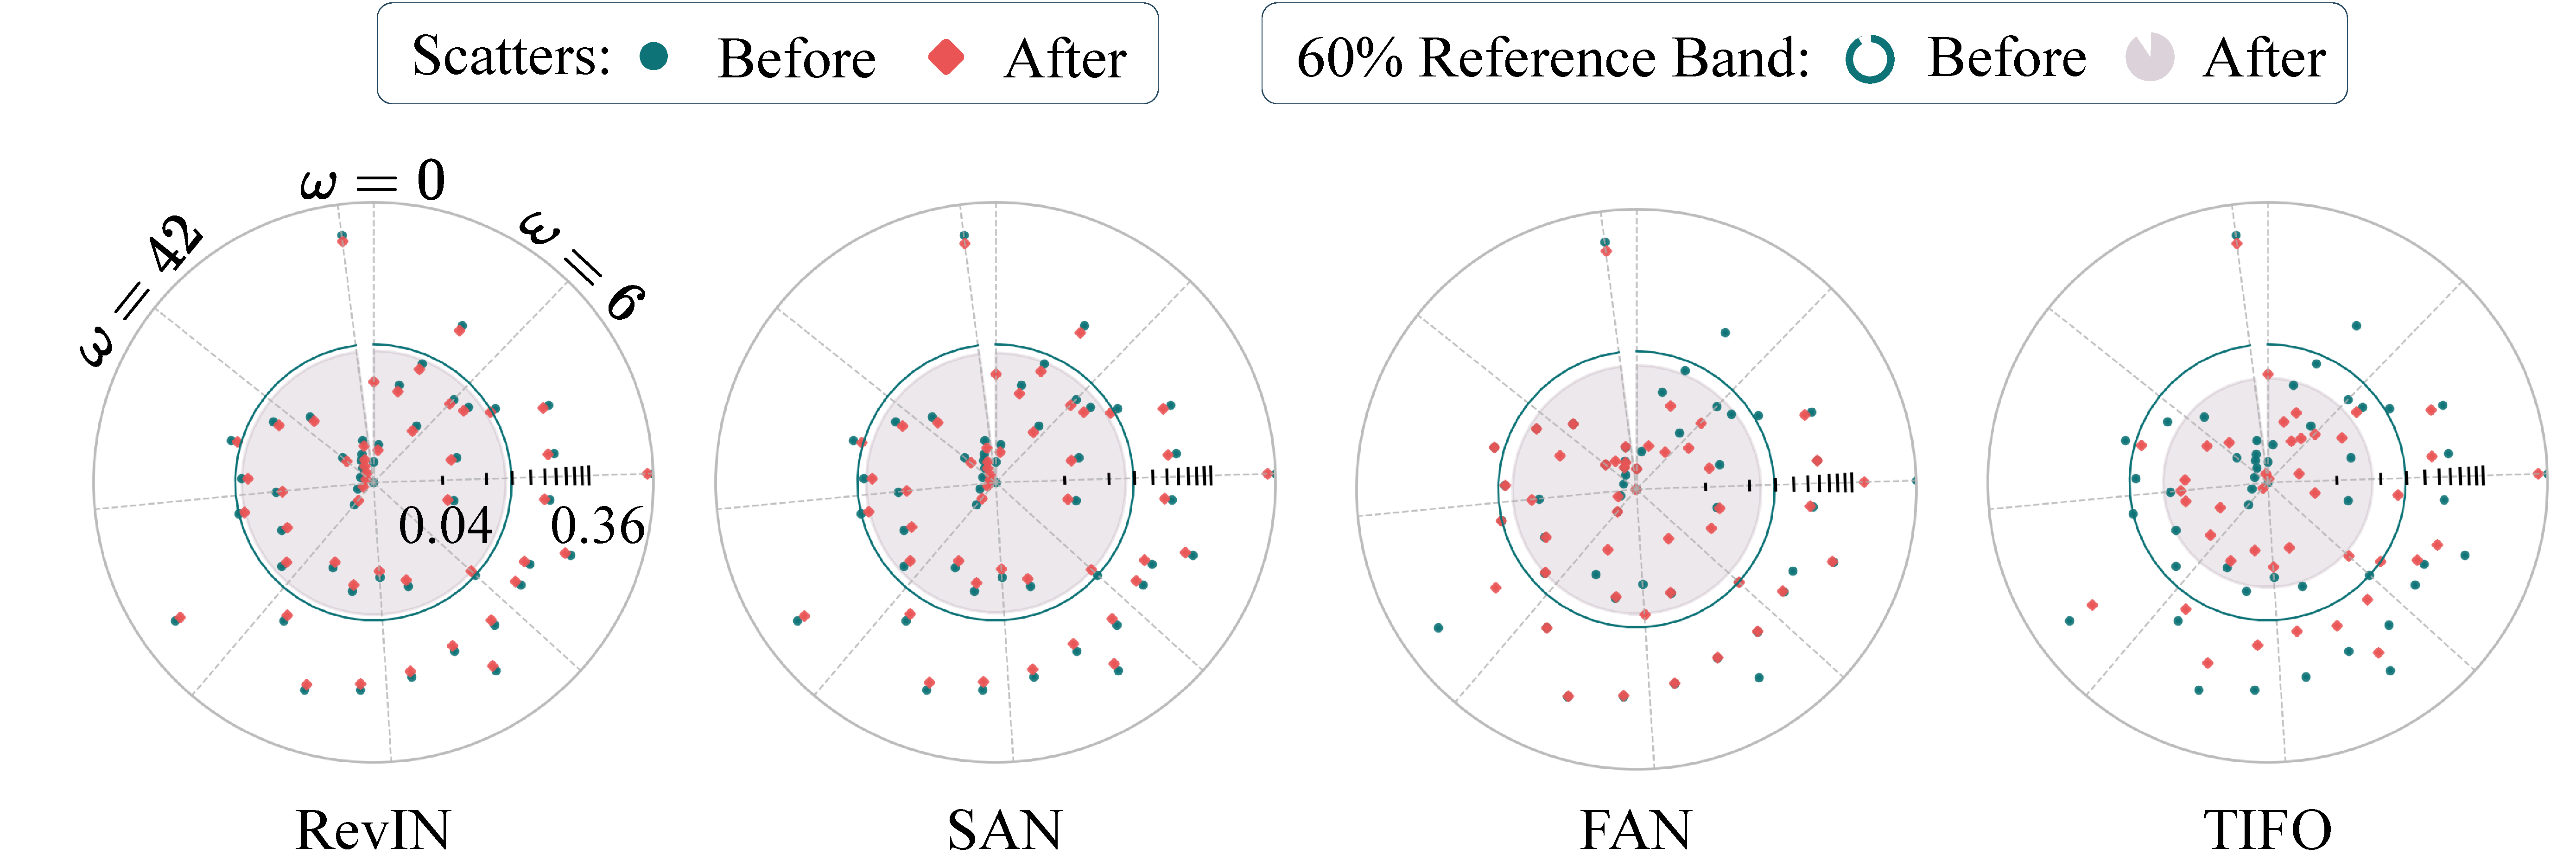
\includegraphics[width=\linewidth]{pics/result_2.pdf}
    \caption{
     \reviewhighlight{Train-Test Distance Compactness: This figure shows a visualization of the JSD$^{2}$ amplitudes distribution distance between the train and test datasets on the electricity data.
     Each scatter point represents one frequency component. 
     A smaller radius indicates a smaller distributional gap.  
     Green and red colors represent the results before and after applying the learning method, respectively.}
     }
    \label{fig:shift_radar}
  \end{minipage} 

  \vspace{1em}

  \begin{minipage}{0.9\linewidth}
    \centering
    \captionsetup{type=table}
    \caption{Frequency‑domain distribution distance between the train and test set.  
    Both the JSD$^{2}$ $(\downarrow)$ and the KS statistic $(\downarrow)$ are computed on amplitudes; bold marks the best per row.}
    \label{tab:freq_dist_flat}
    \resizebox{\textwidth}{!}{%
      \begin{tabular}{l
                      cc  % Raw
                      cc  % Z-score
                      cc  % FAN
                      cc  % SAN
                      cc} % TIFO
        \toprule
        Dataset 
          & \multicolumn{2}{c}{Before} 
          & \multicolumn{2}{c}{ReVIN} 
          & \multicolumn{2}{c}{FAN} 
          & \multicolumn{2}{c}{SAN} 
          & \multicolumn{2}{c}{\method} \\
        \cmidrule(lr){2-3} \cmidrule(lr){4-5} \cmidrule(lr){6-7} \cmidrule(lr){8-9} \cmidrule(lr){10-11}
          & JSD\textsuperscript{2} & KS 
          & JSD\textsuperscript{2} & KS 
          & JSD\textsuperscript{2} & KS 
          & JSD\textsuperscript{2} & KS 
          & JSD\textsuperscript{2} & KS \\
        \midrule
        ETTh1       & 0.36367 & 0.35982 
                    & 0.08100 & 0.08937 
                    & 0.14759 & 0.27057 
                    & 0.04745 & 0.08389 
                    & \textbf{0.04353} & \textbf{0.07357} \\
        % ETTm1       & 0.11677 & 0.15640 
        %             & 0.01983 & 0.07793 
        %             & 0.04603 & 0.12044 
        %             & \textbf{0.01080} & \textbf{0.06470} 
        %             & 0.01620 & 0.07267 \\
        weather     & 0.11156 & 0.19926 
                    & 0.02175 & 0.09172 
                    & 0.05328 & 0.12149 
                    & 0.01739 & 0.09566 
                    & \textbf{0.01687} & \textbf{0.07934} \\
        ECL         & 0.14431 & 0.16804 
                    & 0.08060 & 0.11924 
                    & 0.10394 & 0.16537 
                    & 0.07740 & 0.11639 
                    & \textbf{0.04225} & \textbf{0.09581} \\
        \bottomrule
      \end{tabular}%
    }
  \end{minipage}
\end{figure*}


% \noindent We measure each Fourier component $\omega_j$ using Jensen–Shannon divergence squared (JSD$^{2}$), a symmetric, bounded mean of the forward and reverse KL that reflects the overall information gap, and Kolmogorov–Smirnov statistic (KS), the maximal distance between the empirical cumulative spectra that captures the worst-case mismatch \citep{wang2010KS_test, Detecting_JSD, iqbal2021enhancing_JS}.


\reviewhighlight{Table~\ref{tab:freq_dist_flat} presents the JSD$^2$ and KS statistics for the original data (Before) and after applying RevIN, FAN, SAN, and \method across four benchmark datasets.}
Lower values indicate smaller distributional discrepancies between training and test sets.
On ETTh1, \method reduces JSD$^2$ from 0.3637 to 0.0435 (a reduction of 88\%), and on Electricity from 0.1443 to 0.0423 (71\%). 
KS values also decrease significantly, ranging from 43\% to 80\% reductions across the same datasets.
Figure~\ref{fig:shift_radar} shows the per-frequency JSD$^2$ values on the Electricity dataset. 
Each spoke represents a frequency component, and the gray shadowed circle area serves as a reference band that indicates the region within which $60\%$ of the frequency components fall.
A smaller area reflects a lower overall distributional discrepancy.
\reviewhighlight{As shown in the figure, \method considers all frequency components and significantly reduces distributional differences, achieving effective alignment between training and test datasets.}
RevIN and SAN, which operate in the time domain, 
exhibit minimal changes before and after learning, as evidenced by the near overlap between the green line and the gray reference circle.
FAN, which explicitly operates in the frequency domain, shows improved performance. 
However, it focuses only on the top-$k$ frequency components, affecting only a subset of spokes.  
Overall, \method consistently outperforms all baselines, and more results can be found in Appendix~\ref {appendix:freq_models}.

% apply a unified scaling, leading to a relatively even contraction across the frequency spectrum. 
% FAN zeros out the top-$k$ largest amplitude components, affecting only the corresponding spokes. 
% In contrast, \method learns weights for all frequency components, enabling it to dynamically reduce distributional differences, thereby achieving closer train–test alignment.

%Reference bands shade an area behind the marks in the view between two constant or computed values on the axis.



\noindent\textbf{Fourier Basis Learning Evaluation}
\reviewhighlight{To answer RQ3, after analyzing the impact of \method on the distributional difference, we further investigate how \method affects the deep forecasting models to learn frequency features.}
\reviewhighlight{Figure~\ref{fig:freq_results2} shows the Fourier basis functions in three cases, from left to right are: (i) basis functions before any processing (Before), (ii) after applying FAN, and (iii) after applying \method, respectively.}
We use DLinear as the forecasting model in this evaluation, and results for other models are given in Appendix ~\ref{appendix:freq_models}. 
%The Fourier basis functions $\zeta_{\omega_{1:4}}$ are plotted along the frequency axes. 
The coefficients $\lambda$ of the Fourier basis functions $\zeta_{\omega_{1:4}}$ are $\lambda = 1.0$ in the unprocessed case (Before).
FAN sets the $\lambda$ of the top-$k$ high-amplitude frequencies to zero and leaves the $\lambda$ of the rest frequencies unchanged.
\reviewhighlight{In contrast, \method learns a data-driven $\lambda$ for each basis function.}
The line plots display ground truth and corresponding forecasting results in the frequency domain for each case, with local peak components marked by red diamonds.
Without any processing, the original model failed to capture these local peaks.
FAN, which affects deep forecasting models via frequency modeling, shows improved performance. 
However, it still failed to capture most local peak components.
%FAN only focuses on the largest-amplitude components (e.g., $\omega_1$ and $\omega_2$ in the Figure~\ref{fig:freq_results2}), 
\reviewhighlight{In contrast, after applying the \method, the model successfully captures all four local peak components, outperforms other cases.}
% In the unprocessed case, the model fails to capture these peaks accurately. 
% FAN removes key components, making the forecasting model struggle to capture the local peaks.
% Our dynamic weighting preserves all salient peaks while suppressing noise, allowing the forecasts to capture all four local peaks.



\begin{figure*}[t]
  \centering
  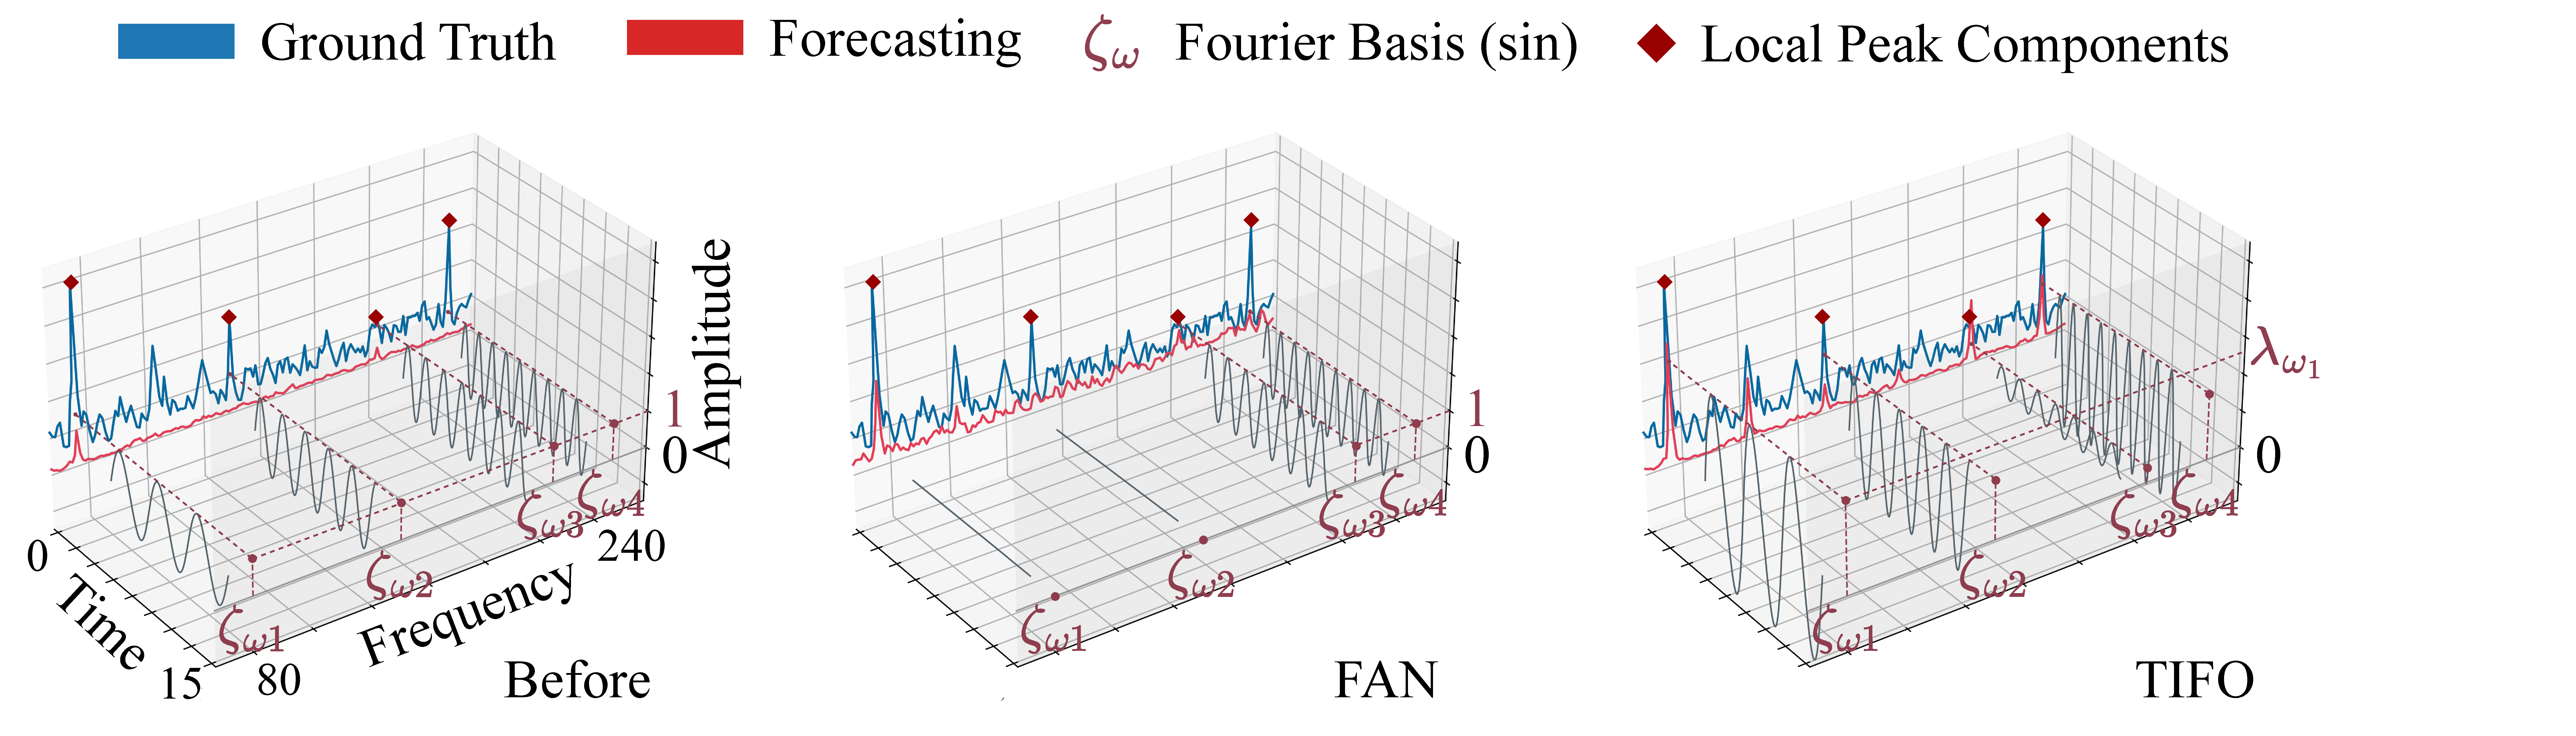
\includegraphics[width=0.9\linewidth]{pics/freq_results2.pdf}
  \caption{Frequency‐domain analysis of Fourier basis Learning. 
  From left to right: unprocessed spectra (Before), after FAN, and after applying \method. 
  Each panel is a 3D box with time, frequency, and amplitude axes. 
  We visualize four Fourier basis waves, $\zeta_{\omega_{1:4}}$, to illustrate how each processing method alters the basis functions. 
  In the frequency–amplitude plane, we plot three forecasting cases: the ground truth in blue and the forecasting results based on the processed input in red. The red diamonds mark key local peak frequencies.
  %Our dynamic weighting preserves all critical peaks while attenuating noise, yielding forecasts that closely match the true spectral peaks.
  }
  \label{fig:freq_results2}
\end{figure*}


\noindent\textbf{Running Time and Ablation Study.}
Table \ref{tab:time_etth1_ettm1} presents the running time results for \method and SAN across two datasets. 
%We compare the running time at the shortest forecasting length ($H=96$) and the longest ($H=720$). 
The results show the average time (in seconds per epoch) using DLinear and PatchTST as backbones. 
\method consistently outperforms SAN across all datasets. 
The full results are in \ref{app:running_time}. 
Notably, we achieved improvements of 60\% to 70\% in 16 out of 28 experiment settings. 
These improvements are primarily because \method only utilizes FFT and MLP during the training phase, minimizing its impact on computation time.
\reviewhighlight{Table~\ref{tab:ablation} shows an ablation in which we replace the computed starting point $s$ with a random vector, while keeping the MLPs and all parameters unchanged.}
\reviewhighlight{This variant assigns random starting points for the MLPs.}
\reviewhighlight{The drop in forecasting accuracy compared to \method demonstrates that initializing the MLPs with $s$ is essential to help deep forecasting models learn the frequency representations.}

  



\begin{table}[t]
\centering
\caption{Running time (s), fixed $L=96$. Speed-ups over +SAN in parentheses.}
\label{tab:time_etth1_ettm1}
%\small
%\setlength{\tabcolsep}{3pt}
\begin{tabular}{c l c c c}
\toprule
\multirow{2}{*}{Model} & Norm & $H$ & ETTh1 & ETTm1 \\
\cmidrule(lr){2-5}
\multirow{4}{*}{\rotatebox[origin=c]{90}{DLinear}}
 & +\method & 96  & \textbf{3.004}{\scriptsize\,(↑65.5\%)} & \textbf{13.456}{\scriptsize\,(↑63.1\%)}\\
 &         & 720 & \textbf{3.082}{\scriptsize\,(↑60.5\%)} & \textbf{13.124}{\scriptsize\,(↑64.2\%)}\\
\cmidrule(lr){2-5}
 & +SAN    & 96  & 8.688 & 36.706\\
 &         & 720 & 8.054 & 36.564\\
\midrule
\multirow{4}{*}{\rotatebox[origin=c]{90}{PatchTST}}
 & +\method & 96  & \textbf{7.952}{\scriptsize\,(↑51.6\%)} & \textbf{54.526}{\scriptsize\,(↑14.3\%)}\\
 &         & 720 & \textbf{8.215}{\scriptsize\,(↑46.2\%)} & \textbf{28.944}{\scriptsize\,(↑56.0\%)}\\
\cmidrule(lr){2-5}
 & +SAN    & 96  & 16.226 & 63.686\\
 &         & 720 & 15.309 & 65.839\\
\bottomrule
\end{tabular}
\end{table}

\begingroup\color{red}
\begin{table}[t]
\centering
\caption{Ablation study (MAE $\downarrow$, mean$\pm$std). Bold = best.}
\label{tab:ablation}
%\small
%\setlength{\tabcolsep}{3pt}
\begin{tabular}{c l c c c}
\toprule
\multirow{2}{*}{Model} & Variant & $H$ & ETTh1 & ETTm1 \\
\cmidrule(lr){2-5}
\multirow{4}{*}{\rotatebox[origin=c]{90}{DLinear}}
 & +\method & 96  & \bf 0.371$\pm$0.032 & \bf 0.299$\pm$0.021\\
 &         & 720 & \bf 0.428$\pm$0.039 & \bf 0.425$\pm$0.032\\
\cmidrule(lr){2-5}
 & +Random & 96  & 0.379$\pm$0.025 & 0.305$\pm$0.022\\
 &         & 720 & 0.435$\pm$0.036 & 0.431$\pm$0.031\\
\midrule
\multirow{4}{*}{\rotatebox[origin=c]{90}{iTransformer}}
 & +\method & 96  & \bf 0.389$\pm$0.023 & \bf 0.330$\pm$0.035\\
 &         & 720 & \bf 0.496$\pm$0.034 & \bf 0.475$\pm$0.043\\
\cmidrule(lr){2-5}
 & +Random & 96  & 0.401$\pm$0.017 & 0.335$\pm$0.033\\
 &         & 720 & 0.502$\pm$0.029 & 0.483$\pm$0.047\\
\bottomrule
\end{tabular}
\end{table}
\endgroup



\noindent \textbf{Frequency modeling ablation studies.}
\reviewhighlight{To verify the effectiveness of our frequency modeling design, we conduct ablation studies on window functions, frequency resolution, and reconstruction strategies, as summarized in Table~\ref{tab:freq_ablation}.}
First, we analyze the sensitivity to window functions and frequency bins $K$ under the original DFT setting (Table~\ref{tab:ablation_window}).
The results demonstrate that utilizing a basic rectangular window with the full spectrum ($K=96$) yields the best performance ($\text{MSE}=0.3938$) with minimal variance.
Applying a Hanning window or reducing the resolution ($K=48$) leads to slight degradation, indicating that preserving the raw global spectral information is preferable.
Second, we compare original \method against Short-Time Fourier Transform (STFT) variants (Table~\ref{tab:ablation_recon}).
Standard STFT configurations with Hanning windows and overlap ($50\%$ or $75\%$) significantly impair accuracy ($\text{MSE} > 0.58$), likely due to boundary artifacts introduced by windowing.
The STFT variant using a $\sqrt{\text{Hann}}$ window fails to outperform the original \method ($\text{MSE}=0.4005$ vs. $0.3938$).
%These findings confirm that the original \method with rectangular windowing is both the simplest and most robust configuration.

% \section{Related Works}
% \textbf{Time-domain normalization methods.}
% Existing methods aim to quantify and explicitly eliminate non-stationary components from both training and test data, thereby aligning distributions and enhancing generalization.
% A normalization is performed by subtracting the empirical mean and dividing by the variance computed from the data.
% At the forecasting stage, denormalization is applied to reintroduce these descriptive statistics to model outputs.
% RevIN \citep{kim2021RevIN} is an innovative work that focuses on z-score normalization.
% Dish-TS \citep{fan2023dish} utilizes learned mean and variance for denormalization.
% SAN \citep{liu2023SAN} models non-stationarity in a set of fine-grained sub-series and proposes an additional loss function to predict their statistics.
% Instead of mean and variance, SIN \citep{han2024sin} proposes an independent neural network to learn features as the objectives of normalization and denormalization adaptively.
% However, existing methods focus on modeling statistical variations in the time domain.
% A recent FAN \citep{ye2024FAN} has taken an initial step in learning predominant frequency components as non-stationarities.
% FAN uses heuristic top-$k$ masking of the largest-amplitude frequencies, zeroing out a subset of components. 
% However, this heuristic selection may risk discarding critical periodic patterns embedded in high-energy regions and introduce sub-optimal frequency correlations into the model, inadvertently misleading the model training.\\
% \textbf{Frequency Domain Modeling.}
% Frequency domain modeling has proven to be highly effective in time series forecasting. 
% Mainstream works employ neural networks to automatically learn frequency representations directly in the raw Fourier domain \citep{Autoformer, ICMLFedformer, LaST, Timesnet, yi2023frequencyMLP}, but such approaches can be vulnerable to noise and to frequency components that vary significantly over time. 
% Some other methods are designed to select informative components via sparse selection \citep{ICMLFedformer, Etsformer, zhou2022film, ye2024FAN} or local normalization in the frequency domain \citep{Piao2024fredformer}, yet these still rely on heuristics, such as top-$k$ selection, or rely on the model to identify the key frequency features.
% In contrast, our method learns and adjusts the coefficients of the Fourier basis functions, naturally encoding the relative importance of different spectral components and allowing seamless deployment on any forecasting backbone.
% Notably, FAN uses heuristic top-$k$ masking of the largest-amplitude frequencies, zeroing out a subset of components. 
% In contrast, \method learns a data-driven coefficient for every Fourier basis function, enabling dynamic weighting of the contribution of each component.
% \subsection{Frequnecy domain models}


\section{Related Works}

\textbf{Time-domain normalization.}
To mitigate distribution shifts, existing methods aim to align distributions by normalizing statistics of each sample.
RevIN \citep{kim2021RevIN} performs instance-wise z-score normalization, while Dish-TS \citep{fan2023dish} utilizes learnable mean and variance parameters.
Further improvements include SAN \citep{liu2023SAN}, which models non-stationarity in fine-grained sub-series, and SIN \citep{han2024sin}, which employs an adaptive network to learn normalization objectives.
%While effective at mitigating mean and variance drift,
%These methods operate strictly in the time domain and process each sample independently.
\reviewhighlight{These methods do not explicitly observe the overall energy distribution of the training set in the frequency domain.}
%Consequently, significant residual train-test shifts often persist in the spectral domain even after time-domain normalization.
\reviewhighlight{In contrast, \method introduces a dataset-level stationarity weighting module.}
\reviewhighlight{By calculating the cross-sample stability of each frequency component across the entire training set, \method explicitly targets the spectral misalignment that remains unaddressed by methods like RevIN.}
% and SAN.

\noindent\textbf{Frequency selection and masking.}
Recognizing the importance of spectral features, recent works have explored selecting informative frequency components.
For instance, FAN \citep{ye2024FAN} takes an initial step by learning predominant frequencies as non-stationarities, employing a heuristic top-$k$ masking strategy to zero out a subset of components based on amplitude.
Similarly, methods like \citet{ICMLFedformer, Etsformer, zhou2022film} utilize sparse attention mechanisms to select frequencies.
However, these methods rely on an attention mechanism or top-$k$ selection derived from the instantaneous high-energy frequencies of a single sample or local window.
%This heuristic selection risks limiting the model to accidentally high-energy frequencies that are unstable at the dataset level, while inadvertently discarding stable but low-energy periodic patterns.
\reviewhighlight{In contrast, \method learns a set of continuous weights for Fourier basis functions based on dataset-level stationarity.}
\reviewhighlight{This allows \method to suppress non-stationary frequencies while preserving stationary signals.}
%, preventing the over-suppression or mis-selection common in heuristic approaches.

% \textbf{Frequency domain models.}
% Frequency domain modeling has proven highly effective for capturing global dependencies in time series.
% Mainstream architectures, such as Autoformer \citep{Autoformer}, Fedformer \citep{ICMLFedformer}, LaST \citep{LaST}, TimesNet \citep{Timesnet}, and FrequencyMLP \citep{yi2023frequencyMLP}, move the primary operators (e.g., attention or convolution) into the frequency domain to enhance long-period modeling capabilities and computational efficiency.
% Similarly, Fredformer \citep{Piao2024fredformer} applies local normalization within the frequency domain.
% These works represent architecture-level designs where the model itself is modified to operate in the spectral domain.
% In contrast, \method is designed as a universal preprocessing layer that is decoupled from the backbone architecture.
% It focuses specifically on learning frequency stationarity rather than altering the core modeling mechanism.
% Therefore, \method is complementary to, rather than repetitive of, these architecture-level frequency domain models.


\begin{table}[t]
\centering
\caption{Ablation on window functions and frequency resolution under the DFT setting (ETTh1, iTransformer).}
\label{tab:ablation_window}
\small
\setlength{\tabcolsep}{4pt}
\begin{tabular}{lcc}
\toprule
Settings & MSE & MAE \\
\midrule
Rect. ($K=48$) & $0.4107 \pm 0.0125$ & $0.4270 \pm 0.0130$ \\
\textbf{Ori (Rect., $K=96$)} & $\mathbf{0.3938 \pm 0.0036}$ & $\mathbf{0.4104 \pm 0.0036}$ \\
Hann ($K=48$) & $0.4117 \pm 0.0015$ & $0.4250 \pm 0.0010$ \\
Hann ($K=96$) & $0.4110 \pm 0.0020$ & $0.4243 \pm 0.0015$ \\
\bottomrule
\end{tabular}
\end{table}

\begin{table}[t]
\centering
\caption{Comparison of frequency decomposition and reconstruction strategies (ETTh1, iTransformer).}
\label{tab:ablation_recon}
\small
\setlength{\tabcolsep}{4pt}
\begin{tabular}{lcc}
\toprule
Strategy & MSE & MAE \\
\midrule
\textbf{Ori (DFT, Rect.)} & $\mathbf{0.3938 \pm 0.0036}$ & $\mathbf{0.4104 \pm 0.0036}$ \\
STFT (Hann, 50\% ovlp) & $0.5820 \pm 0.0174$ & $0.5118 \pm 0.0056$ \\
STFT (Hann, 75\% ovlp) & $0.5814 \pm 0.0166$ & $0.5110 \pm 0.0052$ \\
STFT ($\sqrt{\text{Hann}}$, 50\% ovlp) & $0.4005 \pm 0.0024$ & $0.4148 \pm 0.0024$ \\
\bottomrule
\end{tabular}
\end{table}

\noindent\textbf{Frequency domain models.}
Frequency domain modeling has proven highly effective for capturing global dependencies and improving efficiency.
Mainstream architectures, such as Autoformer \citep{Autoformer}, Fedformer \citep{ICMLFedformer}, TimesNet \citep{Timesnet}, and Frequency MLP \citep{yi2023frequencyMLP}, move primary operators (e.g., attention or convolution) into the frequency domain.
Recent works have further explored spectral properties: FITS \citep{xu2024fits} utilizes frequency interpolation and low-pass filtering for parameter-efficient modeling; FreDF \citep{2025fredf} introduces a frequency-domain loss function to debias direct forecasting against label autocorrelation; and Dynamic Fusion \citep{zhang2024not_all_fre} optimizes the combination of independent frequency predictions.
However, these methods typically focus on optimizing architecture efficiency (FITS), output-side loss constraints (FreDF), or representation expressiveness (Dynamic Fusion). 
They do not explicitly estimate dataset-level frequency statioanrity to guide input adaptation.
In contrast, \method is designed as a universal preprocessing layer decoupled from the backbone architecture.
%It focuses specifically on learning frequency stationarity from training statistics to mitigate input-side spectral distribution shift. 
Therefore, \method is complementary to, rather than repetitive of, these architecture-level frequency domain models.


% We acknowledge that the paper has some limitations:
% (i) \method assumes that the frequency amplitude distributions of the training and test sets are relatively aligned, which generally holds in real-world scenarios but may break under extreme distributional shifts;  
% (ii) \method assumes that the training data span a sufficiently long period to capture all important frequency features, so performance may degrade if the training set is too small.

% This work re-frames non-stationary time-series forecasting as a problem of learning temporally invariant frequency representations.
% % We leverage the Fourier kernel orthonormal basis to sidestep explicit modeling of the latent time distribution, capturing spectral drift that moment-based normalization methods overlook.
% We use the orthonormal Fourier basis to avoid explicitly modeling how the data changes over time, allowing us to detect the distributional shift by learning data-specific eigenvalues.
% This work addresses the distributional shift issue in non-stationary time series forecasting by learning time-invariant frequency representations. 
% %We leverage classical harmonic analysis to decompose signals into orthonormal Fourier basis.
% % Then we infer data-specific eigenvalues that downweight spectral components driving discrepancies between training and testing distributions.
% We introduce \method, which can integrate with popular forecasting models, requires no extra training stages or loss functions, and avoids explicit time distribution modeling.
% %We introduce a lightweight plug-in, \method, that slots into existing forecasters and boosts performance across seven popular datasets. 
% Experiment results show that \method achieves up to $55\%$ MAE reduction and markedly lower train–test distribution difference. 
% Future work will explore the following directions:
% (i) \method assumes that the frequency amplitude distributions of the training and test sets are relatively aligned, which generally holds in real-world scenarios but may break under extreme distributional shifts;  
% (ii) \method assumes that the training data span a sufficiently long period to capture all important frequency features, so performance may degrade if the training set is too small.
% We hope this work will inspire broader integration of harmonic analysis into time series forecasting models.



% Future works will be focus on: 
% (i) It assumes that the frequency amplitude distributions of the training and test sets are similar, which holds for most real‐world datasets but can be influenced by extreme distributional shifts.
% (ii) \method assumes that the training data span a sufficiently long period to capture all important frequency features, so performance may degrade if the training set is too small.
% We expect this approach will inspire broader integration of harmonic analysis insights into time series modeling.

% weakness


%\newpage

% \section{Reproducibility statement}
% \label{sec:Repo}

% To complement the model presented in Section~\ref{subsec:method-overview}, we provide pseudocode and an anonymous repository that illustrate our approach. 
% Algorithm~\ref{alg:compute_scores} shows how frequency-wise stability $s$ is computed from the training data. 
% Algorithm~\ref{alg:apply_weights} demonstrates how these scores are used to adaptively re-weight Fourier coefficients through independent MLP mappings, before transforming back to the time domain.
% The complete implementation, including model training and experimental setup, is available at our anonymous repository:  
% \url{https://anonymous.4open.science/r/TIFO-6BE1}.

% \begin{figure}[h]
%   \centering
%   % -------------------- Left block ---------------------------------
%   \begin{minipage}[t]{0.49\textwidth}
%     \begin{algorithm}
%       \caption{Compute Stability Scores $s_j$}
%       \label{alg:compute_scores}
% \begin{lstlisting}[language=Python,basicstyle=\ttfamily\footnotesize,
%                    keywordstyle=\color{Plum},
%                    commentstyle=\color{PineGreen},
%                    stringstyle=\color{orange},
%                    showstringspaces=false,
%                    columns=fullflexible,tabsize=4,
%                    mathescape=true,escapeinside={(*@}{@*)}]
% def compute_stability_scores(X):
%     """
%     X: (N, T) training set
%     """
%     amp  = np.abs(np.fft.fft(X, axis=1))
%     mean = amp.mean(axis=0)             # per-freq mean
%     std  = amp.std(axis=0) + 1e-5       # per-freq std
%     return mean / std                   # s_j
% \end{lstlisting}
%     \end{algorithm}
%   \end{minipage}\hfill
%   % -------------------- Right block --------------------------------
%   \begin{minipage}[t]{0.49\textwidth}
%     \begin{algorithm}
%       \caption{Apply Fourier Coefficients $\lambda_j$}
%       \label{alg:apply_weights}
% \begin{lstlisting}[language=Python,basicstyle=\ttfamily\footnotesize,
%                    keywordstyle=\color{Plum},
%                    commentstyle=\color{PineGreen},
%                    stringstyle=\color{orange},
%                    showstringspaces=false,
%                    columns=fullflexible,tabsize=4,
%                    mathescape=true,escapeinside={(*@}{@*)}]
% def weight_spectra(x, s, f_cos, f_sin):
%     """ 
%     f_*: learnable MLP layers
%     """
%     X = np.fft.fft(x)
%     X[0::2] *= f_cos(s[0::2])   # re-weight real parts
%     X[1::2] *= f_sin(s[1::2])   # re-weight imag parts
%     return np.fft.ifft(X, n=len(x))
% \end{lstlisting}
%     \end{algorithm}
%   \end{minipage}
% \end{figure}




\section{Conclusion}

\reviewhighlight{Nonstationary time series forecasting suffers from distributional shift due to the different distributions that produce the training and test data.}
As a result, a model trained on the training data may perform poorly on the test data.
\reviewhighlight{These distributions can be regarded as governed by a time structure.}
\reviewhighlight{A time series can be considered as first sampling from a time structure distribution, then from a time-conditional observation distribution.}
\reviewhighlight{Existing methods attempt to alleviate the issue by normalizing the distributions.}
% In this paper, we propose addressing the shift issue by considering cross-sample frequency stationarity across the entire training dataset.
% We demonstrate that the Fourier transform of time series data implicitly induces an eigen-decomposition in the frequency domain by identifying which frequency components are responsible for discrepancies.
\reviewhighlight{To this end, we propose a Time-Invariant Frequency Operator (\method), which learns stationarity-aware weights over the frequency spectrum across the entire dataset.}
%The weight representation highlights stationary frequency components while suppressing non-stationary ones, thereby mitigating the distribution shift issue in time series.
% To justify our method, we show that the Fourier transform of time series data implicitly induces eigen-decomposition in the frequency space.
% Learning the data-specific eigenvalues has the natural interpretation of weighting up frequency components responsible for distributional discrepancies.
\reviewhighlight{Extensive experiments demonstrate that the proposed method achieves superior performance, yielding 18 top-1 and 6 top-2 results out of 28 settings compared to the baselines.}


%%
%% The next two lines define the bibliography style to be used, and
%% the bibliography file.
\bibliographystyle{ACM-Reference-Format}
\bibliography{sample-base}


\newpage
%%
%% If your work has an appendix, this is the place to put it.
\appendix

\section*{Appendix / Supplemental Material}

\DoToC 




\section{Additional Discussions and Details}

\subsection{Additional Discussion about background}
\label{app:more_discussion}





Deep learning models have demonstrated significant success in time series forecasting \citep{long_and_short_KDD19, Informer, Autoformer, liu2022scinet, PatchTST, Crossformer, liu2023itransformer}. 
These models aim to extract diverse and informative patterns from historical observations to enhance the accuracy of future time series predictions. 
To achieve accurate time series predictions, a key challenge is that time series data derived from numerous real-world systems exhibit dynamic and evolving patterns, i.e., a phenomenon known as non-stationarity \citep{stoica2005spectral_book, box2015Timeseriesanalysis, xieIEEEsignle, rhif2019wavelet_non-stationary}. 

\begin{figure}
    \centering
    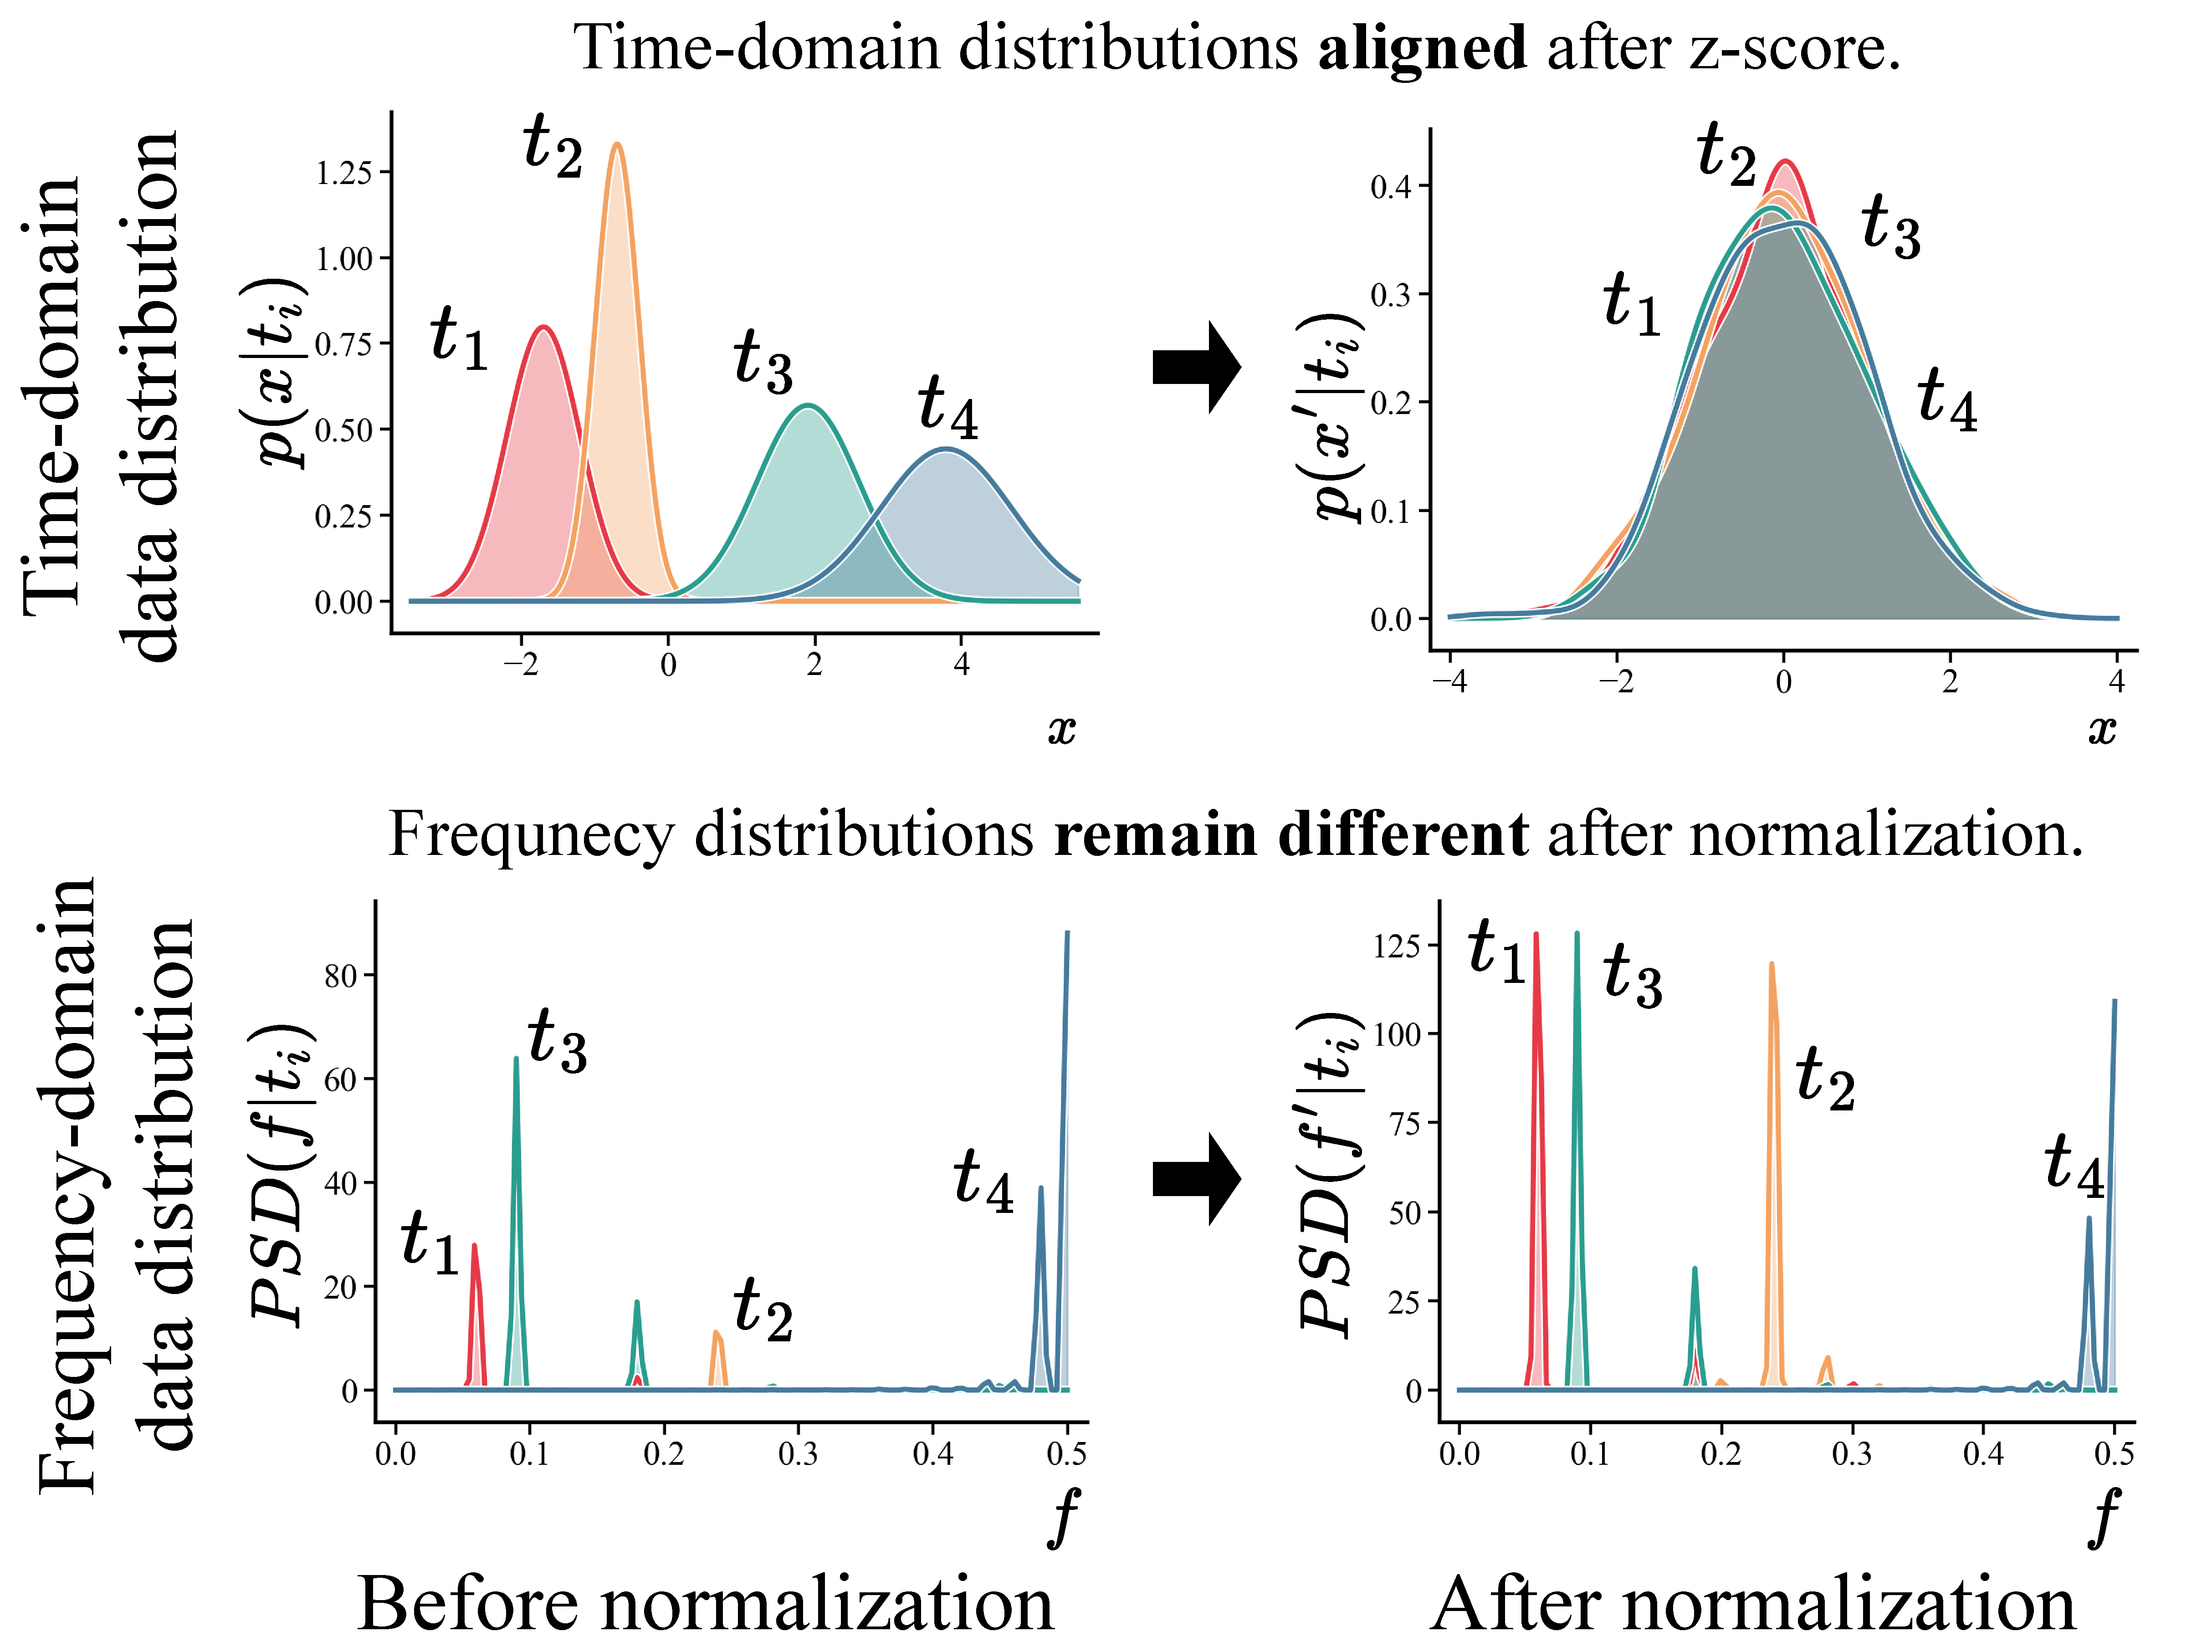
\includegraphics[width=\linewidth]{pics/norm.pdf}
    \caption{
    Illustration of z-score normalization in both time and frequency domains.  
    (Top) Data generating distributions $p(x|t_i)$ across different temporal structures $t_i$ are aligned after $z$-score, sharing a common location and scale.  
    (Bottom) Frequency-domain power spectra before and after $z$-score.
    The frequency-domain distribution remains divergent after normalization.
    }
    \label{fig:norm_weaken_x_on_t}
\end{figure}%


This characteristic typically results in discrepancies among training, testing, and future unseen data distributions. 
Consequently, the non-stationary characteristics of time series data necessitate the development of forecasting models that are robust to such temporal shifts in data distribution, while failing to address this challenge often leads to representation degradation and compromised model generalization \citep{kim2021RevIN, Du2021ADARNN}.




% A recent fashion to tackle the above-mentioned distribution shift issue is leveraging plug-and-play normalization methods \citep{kim2021RevIN, fan2023dish, liu2023SAN, han2024sin}. 
% These methods typically normalize the input time series to a unified distribution, removing non-stationarity explicitly to reduce discrepancies in data distributions. 
% During the forecasting stage, a denormalization is applied, reintroducing the distribution statistics information to the data. 
% This step ensures the forecasting results are accurate while reflecting the inherent variability and fluctuation in the time series, enhancing generalization.
% Since they focus on scaling the inputs and outputs, these methods function as ``model-friendly modules'' that could be easily integrated into various forecasting models without any transformation.
% However, existing works still face several challenges.

% (1) Existing methods model \textit{non-stationary in the time domain} that may not fully capture dynamic and evolving patterns in time series.
% Conceptually, a series of time observations is considered a complex set of waves that varies over time \citep{Digital_Signal_Processing}. 
% These temporal variations, manifested as various frequency waves, are intermixed in the real world \citep{he2023raincoat,Timesnet, Piao2024fredformer}.
% Modeling solely in the time domain struggles to distinguish between different frequency components within superimposed time series, resulting in entangled patterns and sub-optimal performance.
% Recent works have shown that explicitly modeling frequency can enhance representation quality and forecasting accuracy \citep{yi2023frequencyMLP, FRNet2024Zhang, Piao2024fredformer}. (2) Existing methods primarily rely on \textit{z-score normalization} to rescale the input distribution.
To provide more research background details, we conduct a schematic case study using a synthetic time series dataset.
As shown in Figure \ref{fig:norm_weaken_x_on_t}, for each temporal condition $t_i$, we generate $50$ independent samples, each governed by different temporal structures.
Here, we generate different temporal structures by mixing low- and high-frequency components, as shown in the Figure \ref{fig:norm_weaken_x_on_t} (bottom).
For example, $t_1$ mainly contains low-frequency features, while the energy distribution of $t_4$ primarily exists in the high-frequency bands.

Then, we use the numerical distribution of $x$ and the Power Spectral Density (PSD) to evaluate the data distribution in both the time domain and the frequency domain, respectively.
The figure visualizes the data before and after applying z-score normalization. 
In the time domain, normalization successfully transfers the distributions from different $t_i$ into a common Gaussian shape, thereby reducing distributional gaps. 
However, when examining the same data in the frequency domain, we find a very different result: the spectral energy distributions remain distinct and non-overlapping, revealing that the z-score does not address discrepancies in temporal dependencies or frequency compositions. 

This is because the z-score operates only on first- and second-order statistics, ignoring higher-order temporal structure information. 
In contrast, periodicity and other temporal dynamics are preserved in the signal and are clearly reflected in the frequency features. 
In other words, while z-score normalization alters the numerical distribution of the data, it preserves the underlying temporal organization.
Thus, the distribution shift in the frequency domain remains unchanged.

\subsection{Related Works}
% \textbf{Time Series Forecasting.}
% %Forecasting is a fundamental task in time series analysis \citep{tsdata_1, hamilton2020time}. 
% Transformers have demonstrated significant success in time series forecasting \citep{PatchTST, Crossformer, pdformer}, with early works focusing on improving computational efficiency \citep{logtrans2019, longformer, Informer, pyraformer2022} and recent works focusing on modeling temporal dependencies \citep{PatchTST, liu2023itransformer}. 
% Some other works argue that understanding cross-channel correlations is critical for accurate forecasting. \\
\textbf{Time Series Forecasting.} 
Transformer-based architectures have become the mainstream in time series forecasting \citep{PatchTST, Crossformer, pdformer, liu2023itransformer}.
Meanwhile, simple multilayer perceptron (MLP) models, such as DLinear \citep{DLinear, chen2023tsmixer, zhou2022film}, have also attracted attention due to their lower computational costs and forecasting accuracy comparable to transformer-based models.\\
%Approaches utilizing Graph Neural Networks (GNNs) \citep{MTGNN, StemGNN} and channel-wise Transformer-based frameworks like Crossformer \citep{Crossformer} and iTransformer \citep{liu2023itransformer} captures channel-wise dependencies for forecasting.\\
\textbf{Normalization-based Methods.}
Existing methods aim to quantify and explicitly eliminate non-stationary components from both training and test data, thereby aligning distributions and enhancing generalization.
% \hl{Algorithmically, they normalize the input data to remove the distributional statistical differences, such as mean and variance.
% At the forecasting stage, a denormalization is applied to reintroduce these statistical properties to the model outputs.
A normalization is performed by subtracting the empirical mean and dividing by the variance computed from the data.
At the forecasting stage, denormalization is applied to reintroduce these descriptive statistics to model outputs.
% To address distribution shifts in time series forecasting, mainstream methods often use normalization-denormalization techniques to mitigate changes in mean and variance between samples. 
RevIN \citep{kim2021RevIN} is an innovative work that focuses on z-score normalization.
Dish-TS \citep{fan2023dish} utilizes learned mean and variance for denormalization.
SAN \citep{liu2023SAN} models non-stationarity in a set of fine-grained sub-series and proposes an additional loss function to predict their statistics.
Instead of mean and variance, SIN \citep{han2024sin} proposes an independent neural network to learn features as the objectives of normalization and denormalization adaptively.
However, existing methods focus on modeling statistical variations in the time domain.
A recent FAN \citep{ye2024FAN} has taken an initial step in learning predominant frequency components as non-stationarities.
FAN uses heuristic top-$k$ masking of the largest-amplitude frequencies, zeroing out a subset of components. 
However, this heuristic selection may risk discarding critical periodic patterns embedded in high-energy regions and introduce sub-optimal frequency correlations into the model, inadvertently misleading the model training.\\
% \textbf{Frequency Analysis Methods.}
% Incorporating frequency information into models can improve forecasting \citep{Autoformer, ICMLFedformer, LaST, Timesnet, yi2023frequencyMLP}. 
% Recent study \citep{Piao2024fredformer} recognizes a learning bias issue of frequency in the time domain modeling.
% CoST \citep{CoST} proposes a pre-training strategy to learn time-invariant representations in the frequency domain. 
% FiLM \citep{zhou2022film} employs a low-rank approximation method to extract informative frequencies. 
% Koopa \citep{liu2023koopa} introduces Koopman dynamics \citep{koopman1931hamiltonian} to learn time-invariant frequency features.
% While promising, existing methods are costly and architecture-specific, limiting their generalization to other forecasting models.\\
\textbf{Frequency Domain Modeling.}
Frequency domain modeling has proven highly effective in time series forecasting. 
Mainstream works employ neural networks to automatically learn frequency representations directly in the raw Fourier domain \citep{Autoformer, ICMLFedformer, LaST, Timesnet, yi2023frequencyMLP}, but such approaches can be vulnerable to noise and to frequency components that vary significantly over time. 
Some other methods are designed to select informative components via sparse selection \citep{ICMLFedformer, Etsformer, zhou2022film, ye2024FAN} or local normalization in the frequency domain \citep{Piao2024fredformer}, yet these still rely on heuristics, such as top-$k$ selection, or rely on the model to identify the key frequency features.
In contrast, our method learns and adjusts the coefficients of the Fourier basis functions, naturally encoding the relative importance of different spectral components and allowing seamless deployment on any forecasting backbone.
Notably, FAN uses heuristic top-$k$ masking of the largest-amplitude frequencies, zeroing out a subset of components. 
In contrast, \method learns a data-driven coefficient for every Fourier basis function, enabling dynamic weighting of the contribution of each component.


\subsection{Ablation Study on Stationarity Metrics}
\label{app:metric_ablation}

\reviewhighlight{To validate the effectiveness of our proposed stability metric $S(k,c) = \mu_{k,c}/\sigma_{k,c}$ (the reciprocal of the Coefficient of Variation), we conducted an ablation study comparing it against two alternative metrics: Spectral Entropy and Correlation (a proxy for Mutual Information).}

\textbf{Rationale for Metric Selection.}
\reviewhighlight{The core hypothesis of \method is that frequency components exhibiting stable behavior across different samples in the training set are more reliable for generalization.}
\begin{itemize}
    \item \reviewhighlight{\textbf{Coefficient of Variation (CV, ours):} This statistic explicitly measures the dispersion of a variable across multiple observations relative to its mean. In our context, $\mu/\sigma$ quantifies the \textit{cross-sample stationarity}. A high score indicates that a frequency component consistently appears with stable energy across the entire dataset, aligning perfectly with our objective.}
    \item \textbf{Spectral Entropy:} This metric measures the complexity or "spikiness" of the power spectrum within a \textit{single} signal window. While useful for characterizing \textit{intra-sample} complexity, it does not capture how a specific frequency evolves or drifts across the dataset (distribution shift).
    \item \textbf{Mutual Information (MI):} MI measures the dependency between the input frequencies and the forecasting target. While theoretically strong, calculating MI typically requires access to future labels (forecasting targets), making it a supervised signal. Our goal for \method is to serve as an unsupervised, plug-and-play regularization layer that relies solely on input statistics.
\end{itemize}

\textbf{Experimental Results.}
We compared these metrics on the ETTh1 dataset using iTransformer as the backbone. The training was set to a maximum of 30 epochs with early stopping (patience=5).
\begin{itemize}
    \item \texttt{mu\_sigma} (Ours): The default $\mu/\sigma$ metric.
    \item \texttt{entropy}: Inverse spectral entropy (lower entropy $\rightarrow$ higher weight).
    \item \texttt{corr}: The Pearson correlation coefficient $|r|$ between the frequency amplitude and the mean of the future target series, serving as a proxy for Mutual Information.
\end{itemize}

\reviewhighlight{The results are summarized in Table~\ref{tab:metric_ablation}. Our proposed \texttt{mu\_sigma} achieves the best performance in both MSE and MAE.}
\reviewhighlight{Notably, it outperforms \texttt{entropy}, suggesting that consistency across the dataset (cross-sample stationarity) is more critical for handling distribution shift than intra-sample complexity.}
\reviewhighlight{Furthermore, \texttt{mu\_sigma} performs comparably to (or slightly better than) the target-aware \texttt{corr} metric. This confirms that our unsupervised stability score is highly effective and sufficient for identifying robust frequency patterns without requiring label guidance or complex supervised computation.}

\begin{table}[h]
    \centering
    \caption{Comparison of different stationarity metrics on ETTh1 with iTransformer. \textit{mu\_sigma} denotes our default unsupervised metric; \textit{entropy} focuses on intra-sample distribution; \textit{corr} utilizes future labels to approximate Mutual Information.}
    \label{tab:metric_ablation}
    \resizebox{\linewidth}{!}{
        \begin{tabular}{l|l|cc}
            \toprule
            Metric & Description & MSE & MAE \\
            \midrule
            mu\_sigma (\textbf{Ours}) & Mean/Std (Unsupervised, Cross-sample stability) & \textbf{0.3904} & \textbf{0.4071} \\
            entropy & Spectral Entropy (Intra-sample complexity) & 0.3962 & 0.4106 \\
            corr & Correlation $|r|$ (Target-aware, MI approx.) & 0.3948 & 0.4077 \\
            \bottomrule
        \end{tabular}
    }
\end{table}



\subsection{Details of the datasets.}
\label{appendix:exp_datasets}
%%%%%%%% More to appendix%%%%%%%%%%%%%%%%%%%%%%%%%%%%%
Weather contains 21 channels (e.g., temperature and humidity) and is recorded every 10 minutes in 2020. 
ETT \citep{Informer} (Electricity Transformer Temperature) consists of two hourly-level datasets (ETTh1, ETTh2) and two 15-minute-level datasets (ETTm1, ETTm2). 
Electricity \citep{long_and_short_SiGIR18}, from the UCI Machine Learning Repository and preprocessed by, is composed of the hourly electricity consumption of 321 clients in kWh from 2012 to 2014. 
Solar-Energy \citep{long_and_short_SiGIR18} records the solar power production of 137 PV plants in 2006, sampled every 10 minutes.
Traffic contains hourly road occupancy rates measured by 862 sensors on San Francisco Bay area freeways from January 2015 to December 2016.
More details of these datasets can be found in Table.\ref{tab:dataset_overview}.

\begin{table}[h]
\centering
\caption{Overview of Datasets}
\label{tab:dataset_overview}
\resizebox{\linewidth}{!}{
\begin{tabular}{@{}lllll@{}}
\toprule
Dataset & Source & Resolution & Channels & Time Range \\ \midrule
Weather & Autoformer\citep{Autoformer} & Every 10 minutes & 21 (e.g., temperature, humidity) & 2020 \\
ETTh1 & Informer\citep{Informer} & Hourly & 7 states of a electrical transformer & 2016-2017 \\
ETTh2 & Informer\citep{Informer} & Hourly & 7 states of a electrical transformer & 2017-2018 \\
ETTm1 & Informer\citep{Informer} & Every 15 minutes & 7 states of a electrical transformer & 2016-2017 \\
ETTm2 & Informer\citep{Informer} & Every 15 minutes & 7 states of a electrical transformer & 2017-2018 \\
Electricity & UCI ML Repository & Hourly & 321 clients' consumption & 2012-2014 \\
%Solar-Energy & \citep{long_and_short_SiGIR18} & Every 10 minutes & 137 PV plants' production & 2006 \\
Traffic & Informer\citep{Informer} & Hourly & 862 sensors' occupancy & 2015-2016 \\ \bottomrule
\end{tabular}
}
\end{table}





\subsection{Preprocessing and Evaluation details}
\label{appendix:preprocess_detailes}


% We follow the Time-Series-Library split\footnote{\url{https://github.com/thuml/Time-Series-Library}} (7:2:1) with window lengths $L\!\in\!\{96\}$ and apply per-variable $z$-score normalisation.
% Models are trained with MSE loss and assessed by MSE and MAE.  
Given the raw multivariate time‐series data $X\in\mathbb{R}^{T\times C}$, we first slide a window of length $L=96$ over $X$ with stride 1.  
This produces overlapping segments $W=\{\,X_{i:i+L-1}\mid i=1,\dots,T-L+1\}$.  
Each segment is of shape $(L,C)$.  
We order the segments chronologically and split $W$ into training ($70 \%$), validation ($20 \%$), and test ($10 \%$) sets.  
On the training set, we compute per‐variable means $\mu_j$ and standard deviations $\sigma_j$ for $j=1,\dots,C$.  
We then apply per‐variable $z$‐score normalization to every segment in all splits:  
$\tilde w_{i,j} = \frac{w_{i,j} - \mu_j}{\sigma_j},\quad
\forall w\in W,\;i=\{1,\dots,L\},\;j=\{1,\dots,C\}.$  
The normalized segments form $\mathcal{D}_{\mathrm{train}}$, $\mathcal{D}_{\mathrm{val}}$, and $\mathcal{D}_{\mathrm{test}}$, ready for model training and evaluation.

\begin{algorithm}
  \caption{Pre-processing for Time‐Series Forecasting}
  \label{alg:preproc2}
  \KwIn{Time‐series $X\in\mathbb{R}^{T\times C}$, window length $L$, split ratios $(0.7,0.2,0.1)$}
  \KwOut{Normalized sets $\mathcal{D}_{\mathrm{train}},\mathcal{D}_{\mathrm{val}},\mathcal{D}_{\mathrm{test}}$}
  Slice $X$ into overlapping windows  
  $\;W\gets\{X_{i:i+L-1}\mid i=1,\dots,T-L+1\}$\;
  Split $W$ into train/val/test by first 70\%, next 20 \%, last 10 \%\;
  Compute $\mu_j=\mathrm{mean}\bigl(\{w_{i,j}\mid w\in\mathcal{D}_{\mathrm{train}}\}\bigr)$\;
  Compute $\sigma_j=\mathrm{std}\bigl(\{w_{i,j}\mid w\in\mathcal{D}_{\mathrm{train}}\}\bigr)$\;
  \ForEach{segment $w\in W$}{
    \For{variable $j=1,\dots,C$}{
      $\tilde w_{j}\gets (w_{j}-\mu_j)/\sigma_j$\;
    }
    Add $\tilde w$ to its split’s dataset\;
  }
  \Return{$\mathcal{D}_{\mathrm{train}},\,\mathcal{D}_{\mathrm{val}},\,\mathcal{D}_{\mathrm{test}}$}
\end{algorithm}


\subsection{Details of the baselines}
\label{appendix:exp_baselines}

\textbf{Reversible Instance Normalization.}
Reversible Instance Normalization (Revin) normalizes each input sample using z-score normalization while preserving the original mean and variance. 
%After model forecasting,
Revin reverses the normalization to model outputs by using the saved statistics and applies learnable scaling and shifting parameters ($\gamma$ and $\beta$). 
%to enhance the forecast accuracy.

% \begin{algorithm}[t]
%   \caption{Reversible Instance Normalization (Revin)}
%   \label{alg:revin}
%   \small
%   \begin{algorithmic}[1]
%     \State \textbf{Input:} Time-series data $X$, Forecasting model $\mathcal{F}$
%     \State \textbf{Output:} Forecasted data $\hat{X}$
%     \For{each instance $X_i$ in $X$}
%         \State Compute mean $\mu_i \gets \text{mean}(X_i)$\;
%         \State Compute variance $\sigma_i^2 \gets \text{variance}(X_i)$
%         \State Normalize $\tilde{X}_i \gets \frac{X_i - \mu_i}{\sigma_i}$
%         \State \textbf{Store} $\mu_i$ and $\sigma_i^2$
%     \EndFor
%     \State $\tilde{X} \gets \{\tilde{X}_1, \tilde{X}_2, \ldots, \tilde{X}_N\}$
%     \State $\tilde{Y} \gets \mathcal{F}(\tilde{X})$
%     \For{each forecasted instance $\tilde{Y}_i$}
%         \State Reverse Normalize $Y_i \gets \tilde{Y}_i \times \sigma_i + \mu_i$
%         \State Apply learnable parameters $Y_i \gets \gamma \times Y_i + \beta$
%     \EndFor
%     \State \textbf{return} $\hat{X} = \{Y_1, Y_2, \ldots, Y_N\}$
%   \end{algorithmic}
% \end{algorithm}

\textbf{Sequential Adaptive Normalization.} 
Sequential Adaptive Normalization (SAN) has two training phases.
%tackles non-stationary time-series forecasting using a two-phase training approach. 
In the first phase, SAN is trained to learn the relationships between patches of input and target data by mapping their means and variances. 
In the second phase, SAN parameters are frozen, and only the forecasting model is trained. During inference, input data is normalized using SAN, and the model output is reverse-normalized with predicted statistics by SAN.

\textbf{Frequency Adaptive Normalization (FAN)} is a deep learning approach for time series forecasting that decomposes input sequences into frequency components using FFT/RFFT. The algorithm separates the top-k dominant frequency components from residual signals, then employs an MLPfreq network to model the main frequency patterns while handling residuals separately. By processing frequency and temporal information through parallel pathways and combining them via learnable weights, FAN achieves improved forecasting accuracy through frequency-domain feature extraction and adaptive normalization. The method is particularly effective for capturing periodic patterns and long-term dependencies in time series data.

\begin{algorithm}[h]
  \caption{Reversible Instance Normalization (Revin)}
  \label{alg:revin}
  % \small
  % \begin{algorithmic}[1]
     % \textbf{Input:} 
     \KwIn{
     Time-series data $X$, Forecasting model $\mathcal{F}$} 
     \textbf{Output:} Forecasted data $\hat{X}$ \;
    \For{each instance $X_i$ in $X$}
         {
         Compute mean $\mu_i \gets \text{mean}(X_i)$\;
         Compute variance $\sigma_i^2 \gets \text{variance}(X_i)$ \;
         Normalize $\tilde{X}_i \gets \frac{X_i - \mu_i}{\sigma_i}$\;
         \textbf{Store} $\mu_i$ and $\sigma_i^2$ \;
         }
    % \EndFor
     $\tilde{X} \gets \{\tilde{X}_1, \tilde{X}_2, \ldots, \tilde{X}_N\}$ \;
     $\tilde{Y} \gets \mathcal{F}(\tilde{X})$ \;
    \For{each forecasted instance $\tilde{Y}_i$}
    {
         Reverse Normalize $Y_i \gets \tilde{Y}_i \times \sigma_i + \mu_i$ \;
         Apply learnable parameters $Y_i \gets \gamma \times Y_i + \beta$ \;
     }
    % \EndFor
     \textbf{return} $\hat{X} = \{Y_1, Y_2, \ldots, Y_N\}$ \;
  % \end{algorithmic}
\end{algorithm}


\begin{algorithm}[h]
  \caption{Sequential Adaptive Normalization (SAN)}
  \label{alg:san}
  % \small
  % \begin{algorithmic}[1]
     \textbf{Stage 1: Train SAN}\;
     \KwIn{Training data $X$ and targets $Y$
     Divide $X$ and $Y$ into patches $\{X_p\}$ and $\{Y_p\}$
     }
    \For{each pair of patches $(X_p, Y_p)$}
    {
         Compute means $\mu_X \gets \text{mean}(X_p)$, $\mu_Y \gets \text{mean}(Y_p)$ \;
         Compute variances $\sigma_X^2 \gets \text{variance}(X_p)$, $\sigma_Y^2 \gets \text{variance}(Y_p)$ \;
         Train SAN to map $(\mu_X, \sigma_X^2)$ to $(\mu_Y, \sigma_Y^2)$ using loss on $\mu_Y$ and $\sigma_Y^2$ \;
     \textbf{Stage 2: Train Forecasting Model}
     Freeze SAN parameters\;
    \For{each training iteration}
         {Divide input $X$ into patches $\{X_p\}$ \;
        \For{each patch $X_p$}
        {
             Normalize $X_p \gets \frac{X_p - \mu_X}{\sigma_X}$ using SAN's learned $\mu_X$ and $\sigma_X^2$
        % \EndFor
        }
         Forecast $\tilde{Y} \gets \mathcal{F}(X)$ \;
         Divide $\tilde{Y}$ into patches $\{\tilde{Y}_p\}$ \;
        \For{each forecasted patch $\tilde{Y}_p$}
             {Predict $\mu_Y$, $\sigma_Y^2$ using SAN
             Reverse Normalize $Y_p \gets \tilde{Y}_p \times \sigma_Y + \mu_Y$
             }
        % \EndFor
        }
         Compute loss $\mathcal{L}(Y, \hat{Y})$ \;
         Update forecasting model parameters $\theta$ via backpropagation \;
         }
    % \EndFor
     \textbf{return} Trained forecasting model  $\mathcal{F}$ \;
  % \end{algorithmic}
\end{algorithm}


\begin{algorithm}[h]
  \caption{Frequency Adaptive Normalization (FAN)}
  \label{alg:fan}
  
  \textbf{Stage 1: Frequency Decomposition}\;
  \KwIn{Input sequence $x \in \mathbb{R}^{B \times T \times N}$, top-k frequency components $k$, RFFT flag}
  
  \textbf{Function} \textsc{MainFreqPart}$(x, k, \text{rfft})$\;
  \eIf{rfft = True}{
    $x_f \gets \text{RFFT}(x, \text{dim}=1)$ \;
  }{
    $x_f \gets \text{FFT}(x, \text{dim}=1)$ \;
  }
  
  $\text{indices} \gets \text{TopK}(|x_f|, k, \text{dim}=1)$ \;
  $\text{mask} \gets \text{zeros\_like}(x_f)$ \;
  $\text{mask.scatter}(\text{indices}, 1)$ \;
  $x_f^{\text{filtered}} \gets x_f \odot \text{mask}$ \;
  
  \eIf{rfft = True}{
    $x^{\text{filtered}} \gets \text{IRFFT}(x_f^{\text{filtered}}, \text{dim}=1)$ \;
  }{
    $x^{\text{filtered}} \gets \text{IFFT}(x_f^{\text{filtered}}, \text{dim}=1)$ \;
  }
  
  $x^{\text{residual}} \gets x - x^{\text{filtered}}$ \;
  \textbf{return} $x^{\text{residual}}, x^{\text{filtered}}$ \;
  
  \vspace{0.3cm}
  \textbf{Stage 2: Train FAN Model}\;
  \KwIn{Training data $X$, sequence length $T$, prediction length $O$, channels $N$, freq\_topk $k$}
  
  Initialize MLPfreq model $\mathcal{M}_{\text{freq}}$ with parameters $\theta_{\text{freq}}$ \;
  Initialize learnable weights $w \in \mathbb{R}^{2 \times N}$ \;
  
  \For{each training iteration}{
    \textbf{Normalization Phase:}\;
    $(x^{\text{residual}}, x^{\text{filtered}}) \gets \textsc{MainFreqPart}(X, k, \text{rfft})$ \;
    $\hat{x}^{\text{main}} \gets \mathcal{M}_{\text{freq}}(x^{\text{filtered}}, X)$ \;
    
    \textbf{Forward Pass:}\;
    $x^{\text{norm}} \gets x^{\text{residual}}$ \;
    
    \textbf{Denormalization Phase:}\;
    $\hat{x}^{\text{residual}} \gets \text{ForecasterOutput}$ \;
    $\hat{x}^{\text{final}} \gets \hat{x}^{\text{residual}} + \hat{x}^{\text{main}}$ \;
    
    \textbf{Loss Computation:}\;
    $(y^{\text{residual}}, y^{\text{main}}) \gets \textsc{MainFreqPart}(Y_{\text{true}}, k, \text{rfft})$ \;
    $\mathcal{L} \gets \text{MSE}(\hat{x}^{\text{main}}, y^{\text{main}}) + \text{MSE}(\hat{x}^{\text{residual}}, y^{\text{residual}})$ \;
    
    Update parameters $\theta_{\text{freq}}$ and $w$ via backpropagation \;
  }
  
  \vspace{0.3cm}
  \textbf{Stage 3: MLPfreq Architecture}\;
  \KwIn{Main frequency signal $x^{\text{main}} \in \mathbb{R}^{B \times N \times T}$, original input $x \in \mathbb{R}^{B \times N \times T}$}
  
  $h_{\text{freq}} \gets \text{ReLU}(\text{Linear}_{T \rightarrow 64}(x^{\text{main}}))$ \;
  $h_{\text{concat}} \gets \text{Concat}([h_{\text{freq}}, x], \text{dim}=-1)$ \;
  $h_{\text{hidden}} \gets \text{ReLU}(\text{Linear}_{(64+T) \rightarrow 128}(h_{\text{concat}}))$ \;
  $\text{output} \gets \text{Linear}_{128 \rightarrow O}(h_{\text{hidden}})$ \;
  
  \textbf{return} Trained FAN model with frequency decomposition capability \;
\end{algorithm}

\subsection{Details of the backbones and setup}
\label{appendix:exp_backbones_setup}

In our study, we selected three distinct forecasting models to evaluate the effectiveness of our proposed normalization techniques.
DLinear is an MLP-based model renowned for its lightweight architecture, utilizing two separate multilayer perceptrons (MLPs) to learn the periodic and trend components of the data independently.

PatchTST and iTransformer are both Transformer-based models with unique approaches to handling time-series data.
PatchTST introduces a patching operation that samples each input time series into multiple patches, which are then used as input tokens for the transformer, effectively capturing local temporal patterns.
In contrast, iTransformer emphasizes channel-wise attention by treating the entire sequence of each channel as a transformer token and employing self-attention mechanisms to learn the relationships between different channels. 

For all models, we first compute the starting point (Coefficient of variation) across the entire training dataset, a fixed computational process that typically takes less than five seconds. 
Following this, we apply a simple, parameter-free normalization and denormalization method. 
After normalization, the input data is processed through our custom weighting layer before being fed into the forecasting models. 



\subsection{Other experiments details}
\label{appendix:exp_other_detailes}

\textbf{Loss Function.}
For our experiments, we adhere to a conventional approach by employing the Mean Squared Error (MSE) loss function, implemented as \texttt{nn.MSELoss} in our framework. The MSE loss quantifies the average squared difference between the predicted values and the actual target values, providing a straightforward measure of prediction accuracy. Mathematically, the MSE loss is expressed as
$\mathcal{L}_{\text{MSE}} = \frac{1}{N} \sum_{i=1}^{N} \left( \hat{y}_i - y_i \right)^2$,
where $N$ is the number of samples, $\hat{y}_i$ represents the predicted value, and $y_i$ denotes the true target value for the $i$-th sample. This loss function effectively penalizes larger errors more heavily, encouraging the model to achieve higher precision in its predictions.

\textbf{Computational Resources.}
All experiments were conducted on an NVIDIA RTX A6000 GPU with 48GB of memory, utilizing CUDA version 12.4 for accelerated computation. This high-performance computational setup facilitated efficient training and evaluation of our forecasting models, ensuring timely execution of experiments even with large-scale time-series data.



\section{The Full Results.}




\subsection{Full Long-term Forecasting results.}
\label{app: full_results}

Table \ref{app_table_detailed_results_other_methods} and Table \ref{app_table_detailed_results_FAN} present the full comprehensive results discussed in the main paper. 
This table includes the prediction accuracy outcomes on the [Electricity, ETTh1, ETTh2, ETTm1, ETTm2, Traffic, Weather] dataset, utilizing the [DLinear, PatchTST, iTransformer] as the backbone model. 
We have compared our method against all baseline models across all forecasting horizons ($H \in \{96, 192, 336, 720 \}$). 


\begin{table*}
\centering
\caption{Detailed results of comparing our proposal and other normalization methods. The best results are highlighted in \textbf{bold}. The second best are \uline{underlined}.}
\label{app_table_detailed_results_other_methods}
\resizebox{\textwidth}{!}{

\begin{tabular}{cc|cccccccc|cccccccc|cccccccc}
\toprule
\multicolumn{2}{c|}{Models} & \multicolumn{8}{c|}{DLinear \citep{DLinear}} & \multicolumn{8}{c|}{PatchTST \citep{PatchTST}} & \multicolumn{8}{c}{iTransformer \citep{liu2023itransformer}} 
%& \multicolumn{4}{c}{PatchTST} 
\\
% \multicolumn{1}{c|}{Methods} & \multicolumn{2}{c|}{\textbf{+ Ours}} & \multicolumn{2}{c|}{+ RevIN} & \multicolumn{2}{c|}{+ SIN} & \multicolumn{2}{c|}{\textbf{+ Ours}} & \multicolumn{2}{c|}{+ RevIN} & \multicolumn{2}{c}{+ SIN} \\ 
\multicolumn{2}{c|}{Methods} 
& \multicolumn{2}{c|}{\textbf{+ Ours*}} & \multicolumn{2}{c|}{\textbf{+ Ours}} & \multicolumn{2}{c|}{+ SAN}  & \multicolumn{2}{c|}{+ RevIN}
& \multicolumn{2}{c|}{\textbf{+ Ours*}} & \multicolumn{2}{c|}{\textbf{+ Ours}} & \multicolumn{2}{c|}{+ SAN}  & \multicolumn{2}{c|}{+ RevIN}
& \multicolumn{2}{c|}{\textbf{+ Ours*}} & \multicolumn{2}{c|}{\textbf{+ Ours}} & \multicolumn{2}{c|}{+ SAN}  & \multicolumn{2}{c}{+ RevIN} 
%& \multicolumn{2}{c|}{\textbf{+ Ours}} & \multicolumn{2}{c}{+ RevIN}
\\ 
%\midrule
\multicolumn{2}{c|}{Metric} & MSE & MAE & MSE & MAE & MSE & MAE & MSE & MAE & MSE & MAE & MSE & MAE & MSE & MAE & MSE & MAE & MSE & MAE & MSE & MAE & MSE & MAE & MSE & MAE \\ 
\midrule
\multirow{4}{*}{\rotatebox{90}{Electricity}}
            & 96 
            & \textbf{0.135} & \textbf{0.230} & {0.140} & {0.237} & \uline{0.137} & \uline{0.234} & 0.210 & 0.278 
            & \textbf{0.175} & \textbf{0.266} & {0.190} & 0.280 & \uline{0.182} & \uline{0.271} & 0.212 & 0.297  
            & \uline{0.145} & \uline{0.244} & \textbf{0.143} & \textbf{0.237} & 0.171 & 0.262 & 0.152 & 0.251   
            %& \textbf{0.183} & \textbf{0.276} & 0.190 & 0.280 
            \\
            
            & 192 
            & \textbf{0.149} & \textbf{0.245} & {0.155} & {0.249} & \uline{0.151} & \uline{0.247} & 0.210 & 0.304   
            & \textbf{0.183} & \textbf{0.273} & {0.195} & {0.286} & \uline{0.186} & \uline{0.276}  & 0.213 & 0.300   
            & \uline{0.169} & \uline{0.266} & \textbf{0.159} & \textbf{0.252} & 0.180 & 0.270  & 0.165 & 0.255  
            %& \textbf{0.191} & \textbf{0.283} & 0.195 & 0.286 
            \\
            
            & 336 
            & \textbf{0.165} & \textbf{0.262} & {0.171} & {0.267} & \uline{0.166} & \uline{0.264} & 0.223 & 0.309 
            & \textbf{0.198} & \textbf{0.289} & 0.211 & 0.301 & \uline{0.200} & \uline{0.290} & 0.227 & 0.314  
            & \uline{0.178} & \uline{0.271} & \textbf{0.172} & \textbf{0.266} & 0.194 & 0.284 & 0.180 & 0.272  
            %& \textbf{0.200} & \textbf{0.297} & 0.211 & 0.301 
            \\
            
            & 720 
            & \textbf{0.198} & \textbf{0.291} & {0.208} & {0.298} & \uline{0.201} & \uline{0.295} & 0.257 & 0.349 
            & \textbf{0.233} & \textbf{0.317} & {0.253} & {0.334} & \uline{0.237} & \uline{0.322} & 0.268 & 0.344  
            & \uline{0.210} & \uline{0.311} & \textbf{0.205} & \textbf{0.295} & 0.237 & 0.319 & 0.227 & 0.312  
            %& \textbf{0.240} & \textbf{0.332} & 0.253 & 0.334 
            \\

\midrule
\multirow{4}{*}{\rotatebox{90}{ETTh1}}
            & 96 
            & \uline{0.375} & \uline{0.398} & \textbf{0.371} & \textbf{0.392} & 0.383 & 0.399 & 0.396 & 0.410  
            & \uline{0.380} & \uline{0.401} & \textbf{0.374} & \textbf{0.395} & 0.387 & 0.405 & 0.392 & 0.413  
            & \textbf{0.380} & \textbf{0.400} & \uline{0.389} & \uline{0.404} & 0.398 & 0.411 & 0.394 & 0.409 
            %& \textbf{0.375} & \textbf{0.394} & 0.378 & 0.398 
            \\
            
            & 192 
            & \uline{0.410} & \uline{0.417} & \textbf{0.404} & \textbf{0.412} & 0.419 & 0.419 & 0.445 & 0.440  
            & \uline{0.442} & \uline{0.439} & \textbf{0.424} & \textbf{0.428} & 0.445 & 0.440 & 0.448 & 0.436   
            & \textbf{0.429} & \textbf{0.427} & \uline{0.447} & \uline{0.440} & 0.438 & 0.435 & 0.460 & 0.449  
            %& \textbf{0.423} & \textbf{0.425} & 0.427 & 0.430 
            \\
            
            & 336 
            & \textbf{0.430} & \textbf{0.427} & \uline{0.426} & \uline{0.426} & 0.437 & 0.432 & 0.487 & 0.465  
            & \textbf{0.480} & \textbf{0.456} & \uline{0.471} & \uline{0.452} & 0.505 & 0.471 & 0.489 & 0.456    
            & \textbf{0.479} & \textbf{0.451} & \uline{0.492} & \uline{0.463} & 0.481 & 0.456 & 0.501 & 0.475 
            %& \textbf{0.466} & \textbf{0.447} & 0.475 & 0.460 
            \\
            
            & 720 
            & \uline{0.437} & \uline{0.455} & \textbf{0.428} & \textbf{0.448} & 0.446 & 0.459 & 0.512 & 0.510  
            & \uline{0.519} & \uline{0.501} & \textbf{0.514} & \textbf{0.500} & 0.527 & 0.507 & 0.525 & 0.503   
            & \textbf{0.491} & \textbf{0.471} & \uline{0.496} & \uline{0.482} & 0.528 & 0.502 & 0.521 & 0.504  
            %& \textbf{0.489} & \textbf{0.485} & 0.514 & 0.500 
            \\

\midrule
\multirow{4}{*}{\rotatebox{90}{ETTh2}}
            & 96 
            & \textbf{0.273} & \textbf{0.335} & \textbf{0.273} & \uline{0.336} & 0.277 & 0.338 & 0.344 & 0.397 
            & \textbf{0.292} & \textbf{0.347} & \uline{0.301} & \uline{0.349} & 0.314 & 0.361 & 0.344 & 0.397 
            & \uline{0.298} & \uline{0.352} & \textbf{0.297} & \textbf{0.345} & 0.302 & 0.354 & 0.300 & 0.349  
            %& \textbf{0.298} & \textbf{0.347} & 0.301 & 0.349 
            \\
            
            & 192 
            & \textbf{0.335} & \textbf{0.374} & \uline{0.336} & \uline{0.376} & 0.340 & 0.378 & 0.485 & 0.481  
            & \uline{0.385} & \uline{0.402} & \textbf{0.380} & \textbf{0.399} & 0.391 & 0.421 & 0.389 & 0.411   
            & \textbf{0.371} & \uline{0.402} & \uline{0.380} & \textbf{0.395} & 0.383 & 0.402 & 0.381 & 0.415  
            %& \textbf{0.375} & \textbf{0.394} & 0.380 & 0.399 
            \\
            
            & 336 
            & {0.361} & {0.399} & \textbf{0.355} & \textbf{0.395} & \uline{0.356} & \uline{0.398} & 0.582 & 0.536  
            & \uline{0.431} & \uline{0.438} & \textbf{0.410} & \textbf{0.424} & 0.444 & 0.466 & 0.437 & 0.451   
            & \uline{0.425} & \uline{0.435} & \textbf{0.420} & \textbf{0.428} & 0.435 & 0.441 & 0.433 & 0.442  
            %& \textbf{0.420} & \textbf{0.336} & 0.421 & 0.434 
            \\
            
            & 720 
            & \uline{0.388} & \uline{0.429} & \textbf{0.384} & \textbf{0.423} & 0.396 & 0.435 & 0.836 & 0.659 
            & \uline{0.429} & \uline{0.461} & \textbf{0.422} & \textbf{0.443} & 0.467 & 0.484 & 0.430 & 0.481   
            & \uline{0.420} & \uline{0.444} & \textbf{0.410} & \textbf{0.432} & 0.448 & 0.457 & 0.426 & 0.445 
            %& \textbf{0.426} & \textbf{0.443} & 0.435 & 0.454 
            \\

\midrule
\multirow{4}{*}{\rotatebox{90}{ETTm1}}
            & 96 
            & \textbf{0.285} & \textbf{0.339} & {0.299} & \uline{0.341} & \uline{0.288} & 0.342 & 0.353 & 0.374  
            & \uline{0.322} & \uline{0.359} & \textbf{0.321} & \textbf{0.362} & 0.325 & 0.361 & 0.353 & 0.374   
            & \textbf{0.326} & \textbf{0.361} & \uline{0.330} & \uline{0.370} & 0.331 & 0.373 & 0.341 & 0.376  
            \\
            
            & 192 
            & \textbf{0.321} & \textbf{0.359} & {0.336} & {0.364} & \uline{0.323} & \uline{0.363} & 0.391 & 0.392  
            & \textbf{0.350} & \textbf{0.379} & {0.365} & {0.388} & \uline{0.355} & \uline{0.381} & 0.391 & 0.401   
            & \textbf{0.365} & \textbf{0.384} & \uline{0.374} & \uline{0.391} & 0.376 & 0.381 & 0.380 & 0.394  
            %& 0.370 & \textbf{0.385} & \textbf{0.365} & 0.388 
            \\
            
            & 336 
            & \textbf{0.355} & \textbf{0.380} & {0.370} & \uline{0.383} & \uline{0.357} & 0.384 & 0.423 & 0.413  
            & \textbf{0.381} & \textbf{0.401} & {0.407} & {0.408} & \uline{0.385} & \uline{0.402} & 0.423 & 0.413   
            & \textbf{0.395} & \textbf{0.403} & \uline{0.408} & \uline{0.414} & 0.412 & 0.418 & 0.419 & 0.418  
            %& \textbf{0.406} & \textbf{0.407} & 0.397 & 0.406 
            \\
            
            & 720 
            & \textbf{0.405} & \textbf{0.411} & {0.425} & \uline{0.414} & \uline{0.409} & 0.415 & 0.486 & 0.449  
            & \textbf{0.446} & \textbf{0.436} & {0.464} & {0.442} & \uline{0.450} & \uline{0.437} & 0.486 & 0.459   
            & \textbf{0.471} & \textbf{0.447} & \uline{0.475} & \uline{0.449} & 0.485 & 0.453 & 0.486 & 0.455  
            %& \textbf{0.463} & \textbf{0.439} & 0.456 & 0.442 
            \\
            
\midrule
\multirow{4}{*}{\rotatebox{90}{ETTm2}}
            & 96 
            & \textbf{0.163} & \uline{0.255} & \uline{0.165} & \textbf{0.254} & 0.166 & 0.258 & 0.194 & 0.293  
            & \textbf{0.177} & \uline{0.272} & \uline{0.179} & \textbf{0.262} & 0.184 & 0.277 & 0.185 & 0.272   
            & \uline{0.178} & \uline{0.272} & \textbf{0.176} & \textbf{0.258} & 0.180 & 0.272 & 0.200 & 0.281  
            %& \textbf{0.179} & \textbf{0.262} & 0.184 & 0.270 
            \\
            
            & 192 
            & \uline{0.222} & \uline{0.300} & \textbf{0.220} & \textbf{0.291} & 0.223 & 0.302 & 0.283 & 0.360  
            & \uline{0.245} & \uline{0.319} & \textbf{0.240} & \textbf{0.300} & 0.249 & 0.325 & 0.252 & 0.320   
            & \uline{0.247} & \uline{0.311} & \textbf{0.241} & \textbf{0.302} & 0.248 & 0.315 & 0.252 & 0.312  
            %& \textbf{0.} & \textbf{0.} & 0.245 & 0.306 
            \\
            
            & 336 
            & \textbf{0.272} & \uline{0.329} & {0.273} & \textbf{0.325} & \textbf{0.272} & {0.331} & 0.371 & 0.450  
            & \textbf{0.298} & \textbf{0.253} & \uline{0.310} & \uline{0.347} & 0.330 & 0.378 & 0.315 & 0.351   
            & \textbf{0.307} & \uline{0.351} & \textbf{0.307} & \textbf{0.347} & 0.308 & 0.352 & 0.314 & 0.352  
            %& \textbf{0.} & \textbf{0.} & 0.312 & 0.350 
            \\
            
            & 720 
            & \textbf{0.365} & \textbf{0.383} & \uline{0.368} & \textbf{0.383} & 0.380 & 0.384 & 0.555 & 0.509 
            & \textbf{0.405} & \textbf{0.401} & \uline{0.409} & \uline{0.404} & 0.423 & 0.431 & 0.415 & 0.408  
            & \textbf{0.409} & \uline{0.403} & \uline{0.410} & \textbf{0.402} & 0.412 & 0.407 & 0.411 & 0.405  
            %& \textbf{0.} & \textbf{0.} & 0.416 & 0.412 
            \\
\midrule
\multirow{4}{*}{\rotatebox{90}{Traffic}}

            & 96 
            & \uline{0.410} & \uline{0.286} & \textbf{0.408} & \textbf{0.277} & 0.412 & 0.288 & 0.648 & 0.396  
            & \textbf{0.497} & \textbf{0.342} & \uline{0.527} & \uline{0.339} & 0.530 & 0.340 & 0.650 & 0.396   
            & \uline{0.400} & \uline{0.271} & \textbf{0.394} & \textbf{0.268} & 0.502 & 0.329 & 0.401 & 0.277  
            %& \textbf{0.} & \textbf{0.} & 0.495 & 0.324 
            \\
            
            & 192 
            & \uline{0.427} & \uline{0.288} & \textbf{0.422} & \textbf{0.283} & 0.429 & 0.297 & 0.598 & 0.370  
            & \textbf{0.499} & {0.339} & \uline{0.502} & \textbf{0.331} & 0.516 & \uline{0.338} & 0.597 & 0.359  
            & {0.470} & {0.319} & \textbf{0.413} & \textbf{0.277} & 0.490 & 0.331 & \uline{0.421} & \uline{0.282}  
            %& \textbf{0.} & \textbf{0.} & 0.495 & 0.322 
            \\
            
            & 336 
            & \uline{0.439} & \uline{0.305} & \textbf{0.436} & \textbf{0.295} & 0.445 & 0.306 & 0.605 & 0.373  
            & \uline{0.520} & {0.349} & \textbf{0.510} & \textbf{0.327} & 0.533 & \uline{0.343} & 0.605 & 0.362  
            & \uline{0.489} & \uline{0.333} & \textbf{0.428} & \textbf{0.283} & 0.512 & 0.341 & 0.434 & 0.389  
            %& \textbf{0.} & \textbf{0.} & 0.510 & 0.327 
            \\
            
            & 720 
            & \textbf{0.454} & \textbf{0.311} & \uline{0.455} & \textbf{0.311} & 0.474 & 0.319 & 0.645 & 0.395  
            & \uline{0.550} & \uline{0.349} & \textbf{0.545} & \textbf{0.345} & 0.575 & 0.367 & 0.642 & 0.381   
            & {0.478} & {0.330} & \textbf{0.463} & \textbf{0.301} & 0.576 & 0.364 & \uline{0.465} & \uline{0.302} 
            %& \textbf{0.} & \textbf{0.} & 0.545 & 0.345 
            \\
\midrule
\multirow{4}{*}{\rotatebox{90}{Weather}}
            & 96 
            & \textbf{0.150} & \textbf{0.208} & {0.162} & {0.212} & \uline{0.152} & \uline{0.210} & 0.196 & 0.256  
            & \uline{0.167} & \uline{0.225} & \textbf{0.166} & \textbf{0.207} & 0.170 & 0.229 & 0.195 & 0.235   
            & \uline{0.165} & \uline{0.221} & \textbf{0.162} & \textbf{0.204} & 0.170 & 0.227 & 0.175 & 0.225   
            %& \textbf{0.173} & \textbf{0.221} & 0.175 & 0.223 
            \\
            
            & 192 
            & \textbf{0.194} & \textbf{0.251} & {0.207} & \textbf{0.251} & \uline{0.196} & 0.254 & 0.238 & 0.299  
            & \textbf{0.208} & \uline{0.263} & \uline{0.216} & \textbf{0.253} & 0.211 & 0.270 & 0.240 & 0.270   
            & \textbf{0.212} & \uline{0.261} & \uline{0.213} & \textbf{0.252} & 0.214 & 0.270 & 0.225 & 0.257  
            %& \textbf{0.} & \textbf{0.} & 0.223 & 0.257 
            \\
            
            & 336 
            & \textbf{0.243} & \uline{0.289} & {0.256} & \textbf{0.288} & \uline{0.246} & 0.294 & 0.281 & 0.330  
            & \textbf{0.255} & \uline{0.301} & {0.273} & \textbf{0.295} & \uline{0.261} & 0.310 & 0.291 & 0.306   
            & \textbf{0.261} & \uline{0.304} & 0.271 & \textbf{0.295} & \uline{0.265} & 0.309 & 0.280 & 0.307  
            %& \textbf{0.} & \textbf{0.} & 0.281 & 0.299 
            \\
            
            & 720 
            & \textbf{0.311} & \uline{0.339} & {0.325} & \textbf{0.337} & \uline{0.315} & 0.346 & 0.346 & 0.384  
            & \textbf{0.326} & \uline{0.349} & \uline{0.351} & \textbf{0.346} & 0.332 & 0.359 & 0.364 & 0.353   
            & \textbf{0.338} & \textbf{0.345} & \uline{0.340} & \uline{0.347} & 0.342 & 0.358 & 0.373 & 0.366  
            %& \textbf{0.} & \textbf{0.} & 0.355 & 0.347 
            \\
            
\bottomrule
\end{tabular}
}
\end{table*}



% \begin{table}[H]
% \centering
% \caption{Detailed results of comparing our proposal and other normalization methods. The best results are highlighted in \textbf{bold}.}
% \label{table:detailed_results_other_methods}
% \resizebox{\textwidth}{!}{

% \begin{tabular}{cc|cccccccc|cccccccc|cccccccc}
% \toprule
% \multicolumn{2}{c|}{Models} & \multicolumn{8}{c|}{DLinear \citep{DLinear}} & \multicolumn{8}{c|}{PatchTST \citep{PatchTST}} & \multicolumn{8}{c}{iTransformer \citep{liu2023itransformer}} 
% %& \multicolumn{4}{c}{PatchTST} 
% \\
% \multicolumn{2}{c|}{Methods} 
% & \multicolumn{2}{c|}{\textbf{+ \method*}} & \multicolumn{2}{c|}{\textbf{+ \method}} & \multicolumn{2}{c|}{+ SAN}  & \multicolumn{2}{c|}{+ RevIN}
% & \multicolumn{2}{c|}{\textbf{+ \method*}} & \multicolumn{2}{c|}{\textbf{+ \method}} & \multicolumn{2}{c|}{+ SAN}  & \multicolumn{2}{c|}{+ RevIN}
% & \multicolumn{2}{c|}{\textbf{+ \method*}} & \multicolumn{2}{c|}{\textbf{+ \method}} & \multicolumn{2}{c|}{+ SAN}  & \multicolumn{2}{c}{+ RevIN} 
% \\ 
% %\midrule
% \multicolumn{2}{c|}{Metric} & MSE & MAE & MSE & MAE & MSE & MAE & MSE & MAE & MSE & MAE & MSE & MAE & MSE & MAE & MSE & MAE & MSE & MAE & MSE & MAE & MSE & MAE & MSE & MAE \\ 
% \midrule
% \multirow{4}{*}{\rotatebox{90}{Electricity}}
%             & 96 
%             & \textbf{0.135} & \textbf{0.230} & {0.140} & {0.237} & \uline{0.137} & \uline{0.234} & 0.210 & 0.278 
%             & \textbf{0.175} & \textbf{0.266} & {0.190} & 0.280 & \uline{0.182} & \uline{0.271} & 0.212 & 0.297  
%             & \uline{0.145} & \uline{0.244} & \textbf{0.143} & \textbf{0.237} & 0.171 & 0.262 & 0.152 & 0.251   
%             %& \textbf{0.183} & \textbf{0.276} & 0.190 & 0.280 
%             \\
            
%             & 192 
%             & \textbf{0.149} & \textbf{0.245} & {0.155} & {0.249} & \uline{0.151} & \uline{0.247} & 0.210 & 0.304   
%             & \textbf{0.183} & \textbf{0.273} & {0.195} & {0.286} & \uline{0.186} & \uline{0.276}  & 0.213 & 0.300   
%             & \uline{0.169} & \uline{0.266} & \textbf{0.159} & \textbf{0.252} & 0.180 & 0.270  & 0.165 & 0.255  
%             %& \textbf{0.191} & \textbf{0.283} & 0.195 & 0.286 
%             \\
            
%             & 336 
%             & \textbf{0.165} & \textbf{0.262} & {0.171} & {0.267} & \uline{0.166} & \uline{0.264} & 0.223 & 0.309 
%             & \textbf{0.198} & \textbf{0.289} & 0.211 & 0.301 & \uline{0.200} & \uline{0.290} & 0.227 & 0.314  
%             & \uline{0.178} & \uline{0.271} & \textbf{0.172} & \textbf{0.266} & 0.194 & 0.284 & 0.180 & 0.272  
%             %& \textbf{0.200} & \textbf{0.297} & 0.211 & 0.301 
%             \\
            
%             & 720 
%             & \textbf{0.198} & \textbf{0.291} & {0.208} & {0.298} & \uline{0.201} & \uline{0.295} & 0.257 & 0.349 
%             & \textbf{0.233} & \textbf{0.317} & {0.253} & {0.334} & \uline{0.237} & \uline{0.322} & 0.268 & 0.344  
%             & \uline{0.210} & \uline{0.311} & \textbf{0.205} & \textbf{0.295} & 0.237 & 0.319 & 0.227 & 0.312  
%             %& \textbf{0.240} & \textbf{0.332} & 0.253 & 0.334 
%             \\

% \midrule
% \multirow{4}{*}{\rotatebox{90}{ETTh1}}
%             & 96 
%             & \uline{0.375} & \uline{0.398} & \textbf{0.371} & \textbf{0.392} & 0.383 & 0.399 & 0.396 & 0.410  
%             & \uline{0.380} & \uline{0.401} & \textbf{0.374} & \textbf{0.395} & 0.387 & 0.405 & 0.392 & 0.413  
%             & \textbf{0.380} & \textbf{0.400} & \uline{0.389} & \uline{0.404} & 0.398 & 0.411 & 0.394 & 0.409 
%             %& \textbf{0.375} & \textbf{0.394} & 0.378 & 0.398 
%             \\
            
%             & 192 
%             & \uline{0.410} & \uline{0.417} & \textbf{0.404} & \textbf{0.412} & 0.419 & 0.419 & 0.445 & 0.440  
%             & \uline{0.442} & \uline{0.439} & \textbf{0.424} & \textbf{0.428} & 0.445 & 0.440 & 0.448 & 0.436   
%             & \textbf{0.429} & \textbf{0.427} & \uline{0.447} & \uline{0.440} & 0.438 & 0.435 & 0.460 & 0.449  
%             %& \textbf{0.423} & \textbf{0.425} & 0.427 & 0.430 
%             \\
            
%             & 336 
%             & \textbf{0.430} & \textbf{0.427} & \uline{0.426} & \uline{0.426} & 0.437 & 0.432 & 0.487 & 0.465  
%             & \textbf{0.480} & \textbf{0.456} & \uline{0.471} & \uline{0.452} & 0.505 & 0.471 & 0.489 & 0.456    
%             & \textbf{0.479} & \textbf{0.451} & \uline{0.492} & \uline{0.463} & 0.481 & 0.456 & 0.501 & 0.475 
%             %& \textbf{0.466} & \textbf{0.447} & 0.475 & 0.460 
%             \\
            
%             & 720 
%             & \uline{0.437} & \uline{0.455} & \textbf{0.428} & \textbf{0.448} & 0.446 & 0.459 & 0.512 & 0.510  
%             & \uline{0.519} & \uline{0.501} & \textbf{0.514} & \textbf{0.500} & 0.527 & 0.507 & 0.525 & 0.503   
%             & \textbf{0.491} & \textbf{0.471} & \uline{0.496} & \uline{0.482} & 0.528 & 0.502 & 0.521 & 0.504  
%             %& \textbf{0.489} & \textbf{0.485} & 0.514 & 0.500 
%             \\

% \midrule
% \multirow{4}{*}{\rotatebox{90}{ETTh2}}
%             & 96 
%             & \textbf{0.273} & \textbf{0.335} & \textbf{0.273} & \uline{0.336} & 0.277 & 0.338 & 0.344 & 0.397 
%             & \textbf{0.292} & \textbf{0.347} & \uline{0.301} & \uline{0.349} & 0.314 & 0.361 & 0.344 & 0.397 
%             & \uline{0.298} & \uline{0.352} & \textbf{0.297} & \textbf{0.345} & 0.302 & 0.354 & 0.300 & 0.349  
%             %& \textbf{0.298} & \textbf{0.347} & 0.301 & 0.349 
%             \\
            
%             & 192 
%             & \textbf{0.335} & \textbf{0.374} & \uline{0.336} & \uline{0.376} & 0.340 & 0.378 & 0.485 & 0.481  
%             & \uline{0.385} & \uline{0.402} & \textbf{0.380} & \textbf{0.399} & 0.391 & 0.421 & 0.389 & 0.411   
%             & \textbf{0.371} & \uline{0.402} & \uline{0.380} & \textbf{0.395} & 0.383 & 0.402 & 0.381 & 0.415  
%             %& \textbf{0.375} & \textbf{0.394} & 0.380 & 0.399 
%             \\
            
%             & 336 
%             & {0.361} & {0.399} & \textbf{0.355} & \textbf{0.395} & \uline{0.356} & \uline{0.398} & 0.582 & 0.536  
%             & \uline{0.431} & \uline{0.438} & \textbf{0.410} & \textbf{0.424} & 0.444 & 0.466 & 0.437 & 0.451   
%             & \uline{0.425} & \uline{0.435} & \textbf{0.420} & \textbf{0.428} & 0.435 & 0.441 & 0.433 & 0.442  
%             %& \textbf{0.420} & \textbf{0.336} & 0.421 & 0.434 
%             \\
            
%             & 720 
%             & \uline{0.388} & \uline{0.429} & \textbf{0.384} & \textbf{0.423} & 0.396 & 0.435 & 0.836 & 0.659 
%             & \uline{0.429} & \uline{0.461} & \textbf{0.422} & \textbf{0.443} & 0.467 & 0.484 & 0.430 & 0.481   
%             & \uline{0.420} & \uline{0.444} & \textbf{0.410} & \textbf{0.432} & 0.448 & 0.457 & 0.426 & 0.445 
%             %& \textbf{0.426} & \textbf{0.443} & 0.435 & 0.454 
%             \\

% \midrule
% \multirow{4}{*}{\rotatebox{90}{ETTm1}}
%             & 96 
%             & \textbf{0.285} & \textbf{0.339} & {0.299} & \uline{0.341} & \uline{0.288} & 0.342 & 0.353 & 0.374  
%             & \uline{0.322} & \uline{0.359} & \textbf{0.321} & \textbf{0.362} & 0.325 & 0.361 & 0.353 & 0.374   
%             & \textbf{0.326} & \textbf{0.361} & \uline{0.330} & \uline{0.370} & 0.331 & 0.373 & 0.341 & 0.376  
%             \\
            
%             & 192 
%             & \textbf{0.321} & \textbf{0.359} & {0.336} & {0.364} & \uline{0.323} & \uline{0.363} & 0.391 & 0.392  
%             & \textbf{0.350} & \textbf{0.379} & {0.365} & {0.388} & \uline{0.355} & \uline{0.381} & 0.391 & 0.401   
%             & \textbf{0.365} & \textbf{0.384} & \uline{0.374} & \uline{0.391} & 0.376 & 0.381 & 0.380 & 0.394  
%             %& 0.370 & \textbf{0.385} & \textbf{0.365} & 0.388 
%             \\
            
%             & 336 
%             & \textbf{0.355} & \textbf{0.380} & {0.370} & \uline{0.383} & \uline{0.357} & 0.384 & 0.423 & 0.413  
%             & \textbf{0.381} & \textbf{0.401} & {0.407} & {0.408} & \uline{0.385} & \uline{0.402} & 0.423 & 0.413   
%             & \textbf{0.395} & \textbf{0.403} & \uline{0.408} & \uline{0.414} & 0.412 & 0.418 & 0.419 & 0.418  
%             %& \textbf{0.406} & \textbf{0.407} & 0.397 & 0.406 
%             \\
            
%             & 720 
%             & \textbf{0.405} & \textbf{0.411} & {0.425} & \uline{0.414} & \uline{0.409} & 0.415 & 0.486 & 0.449  
%             & \textbf{0.446} & \textbf{0.436} & {0.464} & {0.442} & \uline{0.450} & \uline{0.437} & 0.486 & 0.459   
%             & \textbf{0.471} & \textbf{0.447} & \uline{0.475} & \uline{0.449} & 0.485 & 0.453 & 0.486 & 0.455  
%             %& \textbf{0.463} & \textbf{0.439} & 0.456 & 0.442 
%             \\
            
% \midrule
% \multirow{4}{*}{\rotatebox{90}{ETTm2}}
%             & 96 
%             & \textbf{0.163} & \uline{0.255} & \uline{0.165} & \textbf{0.254} & 0.166 & 0.258 & 0.194 & 0.293  
%             & \textbf{0.177} & \uline{0.272} & \uline{0.179} & \textbf{0.262} & 0.184 & 0.277 & 0.185 & 0.272   
%             & \uline{0.178} & \uline{0.272} & \textbf{0.176} & \textbf{0.258} & 0.180 & 0.272 & 0.200 & 0.281  
%             %& \textbf{0.179} & \textbf{0.262} & 0.184 & 0.270 
%             \\
            
%             & 192 
%             & \uline{0.222} & \uline{0.300} & \textbf{0.220} & \textbf{0.291} & 0.223 & 0.302 & 0.283 & 0.360  
%             & \uline{0.245} & \uline{0.319} & \textbf{0.240} & \textbf{0.300} & 0.249 & 0.325 & 0.252 & 0.320   
%             & \uline{0.247} & \uline{0.311} & \textbf{0.241} & \textbf{0.302} & 0.248 & 0.315 & 0.252 & 0.312  
%             %& \textbf{0.} & \textbf{0.} & 0.245 & 0.306 
%             \\
            
%             & 336 
%             & \textbf{0.272} & \uline{0.329} & {0.273} & \textbf{0.325} & \textbf{0.272} & {0.331} & 0.371 & 0.450  
%             & \textbf{0.298} & \textbf{0.253} & \uline{0.310} & \uline{0.347} & 0.330 & 0.378 & 0.315 & 0.351   
%             & \textbf{0.307} & \uline{0.351} & \textbf{0.307} & \textbf{0.347} & 0.308 & 0.352 & 0.314 & 0.352  
%             %& \textbf{0.} & \textbf{0.} & 0.312 & 0.350 
%             \\
            
%             & 720 
%             & \textbf{0.365} & \textbf{0.383} & \uline{0.368} & \textbf{0.383} & 0.380 & 0.384 & 0.555 & 0.509 
%             & \textbf{0.405} & \textbf{0.401} & \uline{0.409} & \uline{0.404} & 0.423 & 0.431 & 0.415 & 0.408  
%             & \textbf{0.409} & \uline{0.403} & \uline{0.410} & \textbf{0.402} & 0.412 & 0.407 & 0.411 & 0.405  
%             %& \textbf{0.} & \textbf{0.} & 0.416 & 0.412 
%             \\
% \midrule
% \multirow{4}{*}{\rotatebox{90}{Traffic}}

%             & 96 
%             & \uline{0.410} & \uline{0.286} & \textbf{0.408} & \textbf{0.277} & 0.412 & 0.288 & 0.648 & 0.396  
%             & \textbf{0.497} & \textbf{0.342} & \uline{0.527} & \uline{0.339} & 0.530 & 0.340 & 0.650 & 0.396   
%             & \uline{0.400} & \uline{0.271} & \textbf{0.394} & \textbf{0.268} & 0.502 & 0.329 & 0.401 & 0.277  
%             %& \textbf{0.} & \textbf{0.} & 0.495 & 0.324 
%             \\
            
%             & 192 
%             & \uline{0.427} & \uline{0.288} & \textbf{0.422} & \textbf{0.283} & 0.429 & 0.297 & 0.598 & 0.370  
%             & \textbf{0.499} & {0.339} & \uline{0.502} & \textbf{0.331} & 0.516 & \uline{0.338} & 0.597 & 0.359  
%             & {0.470} & {0.319} & \textbf{0.413} & \textbf{0.277} & 0.490 & 0.331 & \uline{0.421} & \uline{0.282}  
%             %& \textbf{0.} & \textbf{0.} & 0.495 & 0.322 
%             \\
            
%             & 336 
%             & \uline{0.439} & \uline{0.305} & \textbf{0.436} & \textbf{0.295} & 0.445 & 0.306 & 0.605 & 0.373  
%             & \uline{0.520} & {0.349} & \textbf{0.510} & \textbf{0.327} & 0.533 & \uline{0.343} & 0.605 & 0.362  
%             & \uline{0.489} & \uline{0.333} & \textbf{0.428} & \textbf{0.283} & 0.512 & 0.341 & 0.434 & 0.389  
%             %& \textbf{0.} & \textbf{0.} & 0.510 & 0.327 
%             \\
            
%             & 720 
%             & \textbf{0.454} & \textbf{0.311} & \uline{0.455} & \textbf{0.311} & 0.474 & 0.319 & 0.645 & 0.395  
%             & \uline{0.550} & \uline{0.349} & \textbf{0.545} & \textbf{0.345} & 0.575 & 0.367 & 0.642 & 0.381   
%             & {0.478} & {0.330} & \textbf{0.463} & \textbf{0.301} & 0.576 & 0.364 & \uline{0.465} & \uline{0.302} 
%             %& \textbf{0.} & \textbf{0.} & 0.545 & 0.345 
%             \\
% \midrule
% \multirow{4}{*}{\rotatebox{90}{Weather}}
%             & 96 
%             & \textbf{0.150} & \textbf{0.208} & {0.162} & {0.212} & \uline{0.152} & \uline{0.210} & 0.196 & 0.256  
%             & \uline{0.167} & \uline{0.225} & \textbf{0.166} & \textbf{0.207} & 0.170 & 0.229 & 0.195 & 0.235   
%             & \uline{0.165} & \uline{0.221} & \textbf{0.162} & \textbf{0.204} & 0.170 & 0.227 & 0.175 & 0.225   
%             %& \textbf{0.173} & \textbf{0.221} & 0.175 & 0.223 
%             \\
            
%             & 192 
%             & \textbf{0.194} & \textbf{0.251} & {0.207} & \textbf{0.251} & \uline{0.196} & 0.254 & 0.238 & 0.299  
%             & \textbf{0.208} & \uline{0.263} & \uline{0.216} & \textbf{0.253} & 0.211 & 0.270 & 0.240 & 0.270   
%             & \textbf{0.212} & \uline{0.261} & \uline{0.213} & \textbf{0.252} & 0.214 & 0.270 & 0.225 & 0.257  
%             %& \textbf{0.} & \textbf{0.} & 0.223 & 0.257 
%             \\
            
%             & 336 
%             & \textbf{0.243} & \uline{0.289} & {0.256} & \textbf{0.288} & \uline{0.246} & 0.294 & 0.281 & 0.330  
%             & \textbf{0.255} & \uline{0.301} & {0.273} & \textbf{0.295} & \uline{0.261} & 0.310 & 0.291 & 0.306   
%             & \textbf{0.261} & \uline{0.304} & 0.271 & \textbf{0.295} & \uline{0.265} & 0.309 & 0.280 & 0.307  
%             %& \textbf{0.} & \textbf{0.} & 0.281 & 0.299 
%             \\
            
%             & 720 
%             & \textbf{0.311} & \uline{0.339} & {0.325} & \textbf{0.337} & \uline{0.315} & 0.346 & 0.346 & 0.384  
%             & \textbf{0.326} & \uline{0.349} & \uline{0.351} & \textbf{0.346} & 0.332 & 0.359 & 0.364 & 0.353   
%             & \textbf{0.338} & \textbf{0.345} & \uline{0.340} & \uline{0.347} & 0.342 & 0.358 & 0.373 & 0.366  
%             %& \textbf{0.} & \textbf{0.} & 0.355 & 0.347 
%             \\
            
% \bottomrule
% \end{tabular}
% }
% \end{table}

\begin{table}[ht]
\centering
\caption{Detailed results of comparing \method and FAN. The best results are highlighted in \textbf{bold}. The second best are \uline{underlined}.}
\label{app_table_detailed_results_FAN}
\resizebox{\textwidth}{!}{

\begin{tabular}{cc|cccccccc|cccccccc}
\toprule
\multicolumn{2}{c|}{Models} & \multicolumn{8}{c|}{DLinear \citep{DLinear}} & \multicolumn{8}{c}{iTransformer \citep{liu2023itransformer}} 
%& \multicolumn{4}{c}{PatchTST} 
\\
\multicolumn{2}{c|}{Methods} 
& \multicolumn{2}{c|}{\textbf{+ \method*}} & \multicolumn{2}{c|}{\textbf{+ \method}} & \multicolumn{2}{c|}{+ FAN}  & \multicolumn{2}{c|}{+ RevIN}
& \multicolumn{2}{c|}{\textbf{+ \method*}} & \multicolumn{2}{c|}{\textbf{+ \method}} & \multicolumn{2}{c|}{+ FAN}  & \multicolumn{2}{c}{+ RevIN} 
\\ 
%\midrule
\multicolumn{2}{c|}{Metric} & MSE & MAE & MSE & MAE & MSE & MAE & MSE & MAE & MSE & MAE & MSE & MAE & MSE & MAE & MSE & MAE  \\ 
\midrule
\multirow{4}{*}{\rotatebox{90}{Electricity}}
            & 96 
            & \textbf{0.135} & \textbf{0.230} & \uline{0.140} & \uline{0.237} & {0.146} & {0.248} & 0.210 & 0.278 
            & \uline{0.145} & \uline{0.244} & \textbf{0.143} & \textbf{0.237} & 0.158 & 0.254 & 0.152 & 0.251   
            %& \textbf{0.183} & \textbf{0.276} & 0.190 & 0.280 
            \\
            
            & 192 
            & \textbf{0.149} & \textbf{0.245} & \uline{0.155} & \uline{0.249} & {0.163} & {0.264} & 0.210 & 0.304     
            & \uline{0.169} & \uline{0.266} & \textbf{0.159} & \textbf{0.252} & 0.170 & 0.263  & 0.165 & 0.255  
            %& \textbf{0.191} & \textbf{0.283} & 0.195 & 0.286 
            \\
            
            & 336 
            & \textbf{0.165} & \textbf{0.262} & \uline{0.171} & \uline{0.267} & {0.180} & {0.282} & 0.223 & 0.309  
            & \uline{0.178} & \uline{0.271} & \textbf{0.172} & \textbf{0.266} & 0.183 & 0.281 & 0.180 & 0.272  
            %& \textbf{0.200} & \textbf{0.297} & 0.211 & 0.301 
            \\
            
            & 720 
            & \textbf{0.198} & \textbf{0.291} & \uline{0.208} & \uline{0.298} & {0.216} & {0.316} & 0.257 & 0.349  
            & \uline{0.210} & \uline{0.311} & \textbf{0.205} & \textbf{0.295} & 0.208 & 0.306 & 0.227 & 0.312  
            %& \textbf{0.240} & \textbf{0.332} & 0.253 & 0.334 
            \\

\midrule
\multirow{4}{*}{\rotatebox{90}{ETTh1}}
            & 96 
            & \uline{0.375} & \uline{0.398} & \textbf{0.371} & \textbf{0.392} & 0.414 & 0.431 & 0.396 & 0.410   
            & \textbf{0.380} & \textbf{0.400} & \uline{0.389} & \uline{0.404} & 0.425 & 0.434 & 0.394 & 0.409 
            %& \textbf{0.375} & \textbf{0.394} & 0.378 & 0.398 
            \\
            
            & 192 
            & \uline{0.410} & \uline{0.417} & \textbf{0.404} & \textbf{0.412} & 0.446 & 0.451 & 0.445 & 0.440     
            & \textbf{0.429} & \textbf{0.427} & \uline{0.447} & \uline{0.440} & 0.483 & 0.468 & 0.460 & 0.449  
            %& \textbf{0.423} & \textbf{0.425} & 0.427 & 0.430 
            \\
            
            & 336 
            & \textbf{0.430} & \textbf{0.427} & \uline{0.426} & \uline{0.426} & 0.476 & 0.474 & 0.487 & 0.465     
            & \textbf{0.479} & \textbf{0.451} & \uline{0.492} & \uline{0.463} & 0.528 & 0.495 & 0.501 & 0.475 
            %& \textbf{0.466} & \textbf{0.447} & 0.475 & 0.460 
            \\
            
            & 720 
            & \uline{0.437} & \uline{0.455} & \textbf{0.428} & \textbf{0.448} & 0.539 & 0.538 & 0.512 & 0.510    
            & \textbf{0.491} & \textbf{0.471} & \uline{0.496} & \uline{0.482} & 0.582 & 0.555 & 0.521 & 0.504  
            %& \textbf{0.489} & \textbf{0.485} & 0.514 & 0.500 
            \\

\midrule
\multirow{4}{*}{\rotatebox{90}{ETTh2}}
            & 96 
            & \textbf{0.273} & \textbf{0.335} & \textbf{0.273} & \uline{0.336} & 0.316 & 0.376 & 0.344 & 0.397  
            & \uline{0.298} & \uline{0.352} & \textbf{0.297} & \textbf{0.345} & 0.358 & 0.408 & 0.300 & 0.349  
            %& \textbf{0.298} & \textbf{0.347} & 0.301 & 0.349 
            \\
            
            & 192 
            & \textbf{0.335} & \textbf{0.374} & \uline{0.336} & \uline{0.376} & 0.384 & 0.423 & 0.485 & 0.481     
            & \textbf{0.371} & \uline{0.402} & \uline{0.380} & \textbf{0.395} & 0.458 & 0.469 & 0.381 & 0.415  
            %& \textbf{0.375} & \textbf{0.394} & 0.380 & 0.399 
            \\
            
            & 336 
            & {0.361} & {0.399} & \textbf{0.355} & \textbf{0.395} & {0.465} & {0.479} & 0.582 & 0.536   
            & \uline{0.425} & \uline{0.435} & \textbf{0.420} & \textbf{0.428} & 0.570 & 0.533 & 0.433 & 0.442  
            %& \textbf{0.420} & \textbf{0.336} & 0.421 & 0.434 
            \\
            
            & 720 
            & \uline{0.388} & \uline{0.429} & \textbf{0.384} & \textbf{0.423} & 0.671 & 0.596 & 0.836 & 0.659  
            & \uline{0.420} & \uline{0.444} & \textbf{0.410} & \textbf{0.432} & 0.786 & 0.651 & 0.426 & 0.445 
            %& \textbf{0.426} & \textbf{0.443} & 0.435 & 0.454 
            \\

\midrule
\multirow{4}{*}{\rotatebox{90}{ETTm1}}
            & 96 
            & \textbf{0.285} & \textbf{0.339} & \uline{0.299} & \uline{0.341} & {0.302} & 0.352 & 0.353 & 0.374   
            & \textbf{0.326} & \textbf{0.361} & \uline{0.330} & \uline{0.370} & 0.360 & 0.390 & 0.341 & 0.376  
            \\
            
            & 192 
            & \textbf{0.321} & \textbf{0.359} & \uline{0.336} & {0.364} & {0.342} & {0.376} & 0.391 & 0.392    
            & \textbf{0.365} & \textbf{0.384} & \uline{0.374} & \uline{0.391} & 0.398 & 0.408 & 0.380 & 0.394  
            %& 0.370 & \textbf{0.385} & \textbf{0.365} & 0.388 
            \\
            
            & 336 
            & \textbf{0.355} & \textbf{0.380} & \uline{0.370} & \uline{0.383} & {0.385} & 0.402 & 0.423 & 0.413   
            & \textbf{0.395} & \textbf{0.403} & \uline{0.408} & \uline{0.414} & 0.435 & 0.436 & 0.419 & 0.418  
            %& \textbf{0.406} & \textbf{0.407} & 0.397 & 0.406 
            \\
            
            & 720 
            & \textbf{0.405} & \textbf{0.411} & \uline{0.425} & \uline{0.414} & {0.442} & 0.439 & 0.486 & 0.449     
            & \textbf{0.471} & \textbf{0.447} & \uline{0.475} & \uline{0.449} & 0.503 & 0.478 & 0.486 & 0.455  
            %& \textbf{0.463} & \textbf{0.439} & 0.456 & 0.442 
            \\
            
\midrule
\multirow{4}{*}{\rotatebox{90}{ETTm2}}
            & 96 
            & \textbf{0.163} & \uline{0.255} & \uline{0.165} & \textbf{0.254} & 0.170 & 0.262 & 0.194 & 0.293     
            & \uline{0.178} & \uline{0.272} & \textbf{0.176} & \textbf{0.258} & 0.195 & 0.293 & 0.200 & 0.281  
            %& \textbf{0.179} & \textbf{0.262} & 0.184 & 0.270 
            \\
            
            & 192 
            & \uline{0.222} & \uline{0.300} & \textbf{0.220} & \textbf{0.291} & 0.230 & 0.306 & 0.283 & 0.360    
            & \uline{0.247} & \uline{0.311} & \textbf{0.241} & \textbf{0.302} & 0.276 & 0.350 & 0.252 & 0.312  
            %& \textbf{0.} & \textbf{0.} & 0.245 & 0.306 
            \\
            
            & 336 
            & \textbf{0.272} & \uline{0.329} &\uline{0.273} & \textbf{0.325} & {0.293} & {0.351} & 0.371 & 0.450     
            & \textbf{0.307} & \uline{0.351} & \textbf{0.307} & \textbf{0.347} & 0.336 & 0.385 & 0.314 & 0.352  
            %& \textbf{0.} & \textbf{0.} & 0.312 & 0.350 
            \\
            
            & 720 
            & \textbf{0.365} & \textbf{0.383} & \uline{0.368} & \textbf{0.383} & 0.420 & 0.436 & 0.555 & 0.509   
            & \textbf{0.409} & \uline{0.403} & \uline{0.410} & \textbf{0.402} & 0.539 & 0.512 & 0.411 & 0.405  
            %& \textbf{0.} & \textbf{0.} & 0.416 & 0.412 
            \\
\midrule
\multirow{4}{*}{\rotatebox{90}{Traffic}}

            & 96 
            & \uline{0.410} & \uline{0.286} & \textbf{0.408} & \textbf{0.277} & 0.524 & 0.340 & 0.648 & 0.396  
            & \uline{0.400} & \uline{0.271} & \textbf{0.394} & \textbf{0.268} & 0.525 & 0.341 & 0.401 & 0.277  
            %& \textbf{0.} & \textbf{0.} & 0.495 & 0.324 
            \\
            
            & 192 
            & \uline{0.427} & \uline{0.288} & \textbf{0.422} & \textbf{0.283} & 0.523 & 0.338 & 0.598 & 0.370  
            & {0.470} & {0.319} & \textbf{0.413} & \textbf{0.277} & 0.517 & 0.336 & \uline{0.421} & \uline{0.282}  
            %& \textbf{0.} & \textbf{0.} & 0.495 & 0.322 
            \\
            
            & 336 
            & \uline{0.439} & \uline{0.305} & \textbf{0.436} & \textbf{0.295} & 0.537 & 0.343 & 0.605 & 0.373   
            & \uline{0.489} & \uline{0.333} & \textbf{0.428} & \textbf{0.283} & 0.530 & 0.339 & 0.434 & 0.389  
            %& \textbf{0.} & \textbf{0.} & 0.510 & 0.327 
            \\
            
            & 720 
            & \textbf{0.454} & \textbf{0.311} & \uline{0.455} & \textbf{0.311} & 0.581 & 0.362 & 0.645 & 0.395   
            & {0.478} & {0.330} & \textbf{0.463} & \textbf{0.301} & 0.573 & 0.339 & \uline{0.465} & \uline{0.302} 
            %& \textbf{0.} & \textbf{0.} & 0.545 & 0.345 
            \\
\midrule
\multirow{4}{*}{\rotatebox{90}{Weather}}
            & 96 
            & \textbf{0.150} & \textbf{0.208} & \uline{0.162} & \uline{0.212} & {0.187} & {0.242} & 0.196 & 0.256    
            & \uline{0.165} & \uline{0.221} & \textbf{0.162} & \textbf{0.204} & 0.178 & 0.235 & 0.175 & 0.225   
            %& \textbf{0.173} & \textbf{0.221} & 0.175 & 0.223 
            \\
            
            & 192 
            & \textbf{0.194} & \textbf{0.251} & \uline{0.207} & \textbf{0.251} & {0.227} & 0.280 & 0.238 & 0.299    
            & \textbf{0.212} & \uline{0.261} & \uline{0.213} & \textbf{0.252} & 0.220 & 0.275 & 0.225 & 0.257  
            %& \textbf{0.} & \textbf{0.} & 0.223 & 0.257 
            \\
            
            & 336 
            & \textbf{0.243} & \uline{0.289} & \uline{0.256} & \textbf{0.288} & {0.278} & 0.330 & 0.281 & 0.330     
            & \textbf{0.261} & \uline{0.304} & 0.271 & \textbf{0.295} & \uline{0.267} & 0.314 & 0.280 & 0.307  
            %& \textbf{0.} & \textbf{0.} & 0.281 & 0.299 
            \\
            
            & 720 
            & \textbf{0.311} & \uline{0.339} & \uline{0.325} & \textbf{0.337} & {0.341} & 0.368 & 0.346 & 0.384  
            & \textbf{0.338} & \textbf{0.345} & \uline{0.340} & \uline{0.347} & 0.340 & 0.369 & 0.373 & 0.366  
            %& \textbf{0.} & \textbf{0.} & 0.355 & 0.347 
            \\
            
\bottomrule
\end{tabular}
}
\end{table}


\subsection{Analysis Results}
\label{appendix:freq_models}

\subsubsection{Fourier Distribution Analysis}

In the main text we describe using Jensen–Shannon divergence squared (JSD$^2$) and the Kolmogorov–Smirnov (KS) statistic to quantify spectral distribution shift between training and test sets. 
Here we show another result and the algorithms.

\textbf{JSD$^2$ Computation.}
For each frequency $\omega_j$, let
$a = \bigl\{\,\text{amp}_{i,j}\mid i\in t_{\mathrm{train}}\bigr\},\quad
b = \bigl\{\,\text{amp}_{i,j}\mid i\in t_{\mathrm{test}}\bigr\}.$
We build histograms of $a$ and $b$, normalize to probability mass functions, and compute the Jensen–Shannon divergence squared via the Python Library "SciPy" `jensenshannon` function.

\begin{algorithm}[t]
  \caption{Compute JSD$^2$ between two samples}
  \label{alg:jsd2}
  \KwIn{Arrays $a, b$; number of bins $B$}
  \KwOut{Jensen–Shannon divergence squared $D_{\mathrm{JSD}^2}$}
  $v_{\min} \gets \min(\min a, \min b)$\;
  $v_{\max} \gets \max(\max a, \max b)$\;
  Compute histogram $\,h_a\gets\mathrm{histogram}(a;B,[v_{\min},v_{\max}])$\;
  Compute histogram $\,h_b\gets\mathrm{histogram}(b;B,[v_{\min},v_{\max}])$\;
  Normalize: $p\gets h_a / \sum h_a$, \quad $q\gets h_b / \sum h_b$\;
  $D_{\mathrm{JSD}}\gets \mathrm{jensenshannon}(p,\,q,\;\mathrm{base}=2)$\;
  $D_{\mathrm{JSD}^2}\gets D_{\mathrm{JSD}}^2$\;
  \Return{$D_{\mathrm{JSD}^2}$}
\end{algorithm}


\textbf{KS Statistic Computation.}
For each frequency index $\omega_j$, using the same samples $a$ and $b$, we compute their empirical cumulative distribution functions (ECDFs) and take the maximum absolute difference.

\begin{algorithm}[t]
  \caption{Compute Kolmogorov–Smirnov statistic}
  \label{alg:ks}
  \KwIn{Arrays $a, b$}
  \KwOut{KS statistic $D_{\mathrm{KS}}$}
  Sort $a\to a_{\mathrm{sorted}}$, \quad sort $b\to b_{\mathrm{sorted}}$\;
  Let $\,V\gets \mathrm{unique}(\{a_{\mathrm{sorted}}\}\cup\{b_{\mathrm{sorted}}\})$\;
  \ForEach{$v\in V$}{
    $F_a(v)\gets \tfrac{1}{|a|}\,\bigl|\{x\in a: x\le v\}\bigr|$\;
    $F_b(v)\gets \tfrac{1}{|b|}\,\bigl|\{x\in b: x\le v\}\bigr|$\;
    Compute $\Delta(v)\gets |F_a(v)-F_b(v)|$\;
  }
  $D_{\mathrm{KS}}\gets \max_{v\in V}\Delta(v)$\;
  \Return{$D_{\mathrm{KS}}$}
\end{algorithm}

% \begin{table}[ht]
% \centering
% \caption{Detailed results of comparing our proposal and other normalization methods. The best results are highlighted in \textbf{bold}.}
% \label{table:detailed_results_other_methods}
% \resizebox{\textwidth}{!}{
% \begin{tabular}{cc|cccccccc|cccccccc|cccccccc}
% \toprule
% \multicolumn{2}{c|}{Models} & \multicolumn{8}{c|}{DLinear \citep{DLinear}} & \multicolumn{8}{c|}{PatchTST \citep{PatchTST}} & \multicolumn{8}{c}{iTransformer \citep{liu2023itransformer}} 
% %& \multicolumn{4}{c}{PatchTST} 
% \\
% % \multicolumn{1}{c|}{Methods} & \multicolumn{2}{c|}{\textbf{+ Ours}} & \multicolumn{2}{c|}{+ RevIN} & \multicolumn{2}{c|}{+ SIN} & \multicolumn{2}{c|}{\textbf{+ Ours}} & \multicolumn{2}{c|}{+ RevIN} & \multicolumn{2}{c}{+ SIN} \\ 
% \multicolumn{2}{c|}{Methods} & \multicolumn{2}{c|}{\textbf{+ Ours}} & \multicolumn{2}{c|}{+ SAN}  & \multicolumn{2}{c|}{+ RevIN} & \multicolumn{2}{c|}{Ori} & \multicolumn{2}{c|}{\textbf{+ Ours}} & \multicolumn{2}{c|}{+ SAN}  & \multicolumn{2}{c|}{+ RevIN} & \multicolumn{2}{c|}{Ori} & \multicolumn{2}{c|}{\textbf{+ Ours}} & \multicolumn{2}{c|}{+ SAN} & \multicolumn{2}{c|}{+ RevIN} & \multicolumn{2}{c}{Ori} 
% %& \multicolumn{2}{c|}{\textbf{+ Ours}} & \multicolumn{2}{c}{+ RevIN}
% \\ 
% %\midrule
% \multicolumn{2}{c|}{Metric} & MSE & MAE & MSE & MAE & MSE & MAE & MSE & MAE & MSE & MAE & MSE & MAE & MSE & MAE & MSE & MAE & MSE & MAE & MSE & MAE & MSE & MAE & MSE & MAE \\ 
% \midrule
% \multirow{4}{*}{\rotatebox{90}{Electricity}}
%             & 96 
%             & \textbf{0.140} & \textbf{0.237} & 0.137 & 0.234 & 0.210 & 0.301 & 0.140 & 0.237
%             & \textbf{0.190} & \textbf{0.280} & 0.182 & 0.271 & 0.212 & 0.297 & 0.195 & 0.287 
%             & \textbf{0.143} & \textbf{0.237} & 0.171 & 0.262 & 0.148 & 0.240 & 0.148 & 0.246  
%             %& \textbf{0.183} & \textbf{0.276} & 0.190 & 0.280 
%             \\
            
%             & 192 
%             & \textbf{0.155} & \textbf{0.249} & 0.151 & 0.247 & 0.210 & 0.304  & 0.153 & 0.250 
%             & \textbf{0.195} & \textbf{0.286} & 0.186 & 0.276  & 0.213 & 0.300 & 0.197 & 0.291  
%             & \textbf{0.159} & \textbf{0.252} & 0.180 & 0.270  & 0.264 & 0.255 & 0.164 & 0.261 
%             %& \textbf{0.191} & \textbf{0.283} & 0.195 & 0.286 
%             \\
            
%             & 336 
%             & \textbf{0.171} & \textbf{0.267} & 0.166 & 0.264 & 0.223 & 0.309 & 0.168 & 0.267
%             & \textbf{0.211} & \textbf{0.301} & 0.200 & 0.290 & 0.227 & 0.314 & 0.213 & 0.305 
%             & \textbf{0.172} & \textbf{0.266} & 0.194 & 0.284 & 0.180 & 0.272 & 0.189 & 0.292 
%             %& \textbf{0.200} & \textbf{0.297} & 0.211 & 0.301 
%             \\
            
%             & 720 
%             & \textbf{0.208} & \textbf{0.298} & 0.201 & 0.295 & 0.257 & 0.349 & 0.203 & 0.301
%             & \textbf{0.253} & \textbf{0.334} & 0.237 & 0.322 & 0.268 & 0.344 & 0.265 & 0.343 
%             & \textbf{0.205} & \textbf{0.295} & 0.237 & 0.319 & 0.227 & 0.312 & 0.215 & 0.317 
%             %& \textbf{0.240} & \textbf{0.332} & 0.253 & 0.334 
%             \\

% \midrule
% \multirow{4}{*}{\rotatebox{90}{ETTh1}}
%             & 96 
%             & \textbf{0.371} & \textbf{0.392} & 0.383 & 0.399 & 0.396 & 0.410 & 0.377 & 0.399 
%             & \textbf{0.374} & \textbf{0.395} & 0.387 & 0.405 & 0.392 & 0.413 & 0.398 & 0.420 
%             & \textbf{0.389} & \textbf{0.404} & 0.398 & 0.411 & 0.394 & 0.409 & 0.416 & 0.431
%             %& \textbf{0.375} & \textbf{0.394} & 0.378 & 0.398 
%             \\
            
%             & 192 
%             & \textbf{0.404} & \textbf{0.412} & 0.419 & 0.419 & 0.445 & 0.440 & 0.417 & 0.426 
%             & \textbf{0.424} & \textbf{0.428} & 0.445 & 0.440 & 0.448 & 0.436 & 0.442 & 0.449  
%             & \textbf{0.447} & \textbf{0.440} & 0.438 & 0.435 & 0.460 & 0.449 & 0.473 & 0.465 
%             %& \textbf{0.423} & \textbf{0.425} & 0.427 & 0.430 
%             \\
            
%             & 336 
%             & \textbf{0.426} & \textbf{0.426} & 0.437 & 0.432 & 0.487 & 0.465 & 0.464 & 0.461 
%             & \textbf{0.471} & \textbf{0.452} & 0.505 & 0.471 & 0.489 & 0.456 & 0.525 & 0.517   
%             & \textbf{0.492} & \textbf{0.463} & 0.481 & 0.456 & 0.501 & 0.475 & 0.553 & 0.517
%             %& \textbf{0.466} & \textbf{0.447} & 0.475 & 0.460 
%             \\
            
%             & 720 
%             & \textbf{0.428} & \textbf{0.448} & 0.446 & 0.459 & 0.512 & 0.510 & 0.493 & 0.505 
%             & \textbf{0.514} & \textbf{0.500} & 0.483 & 0.483 & 0.483 & 0.475 & 0.556 & 0.537  
%             & \textbf{0.496} & \textbf{0.482} & 0.528 & 0.502 & 0.521 & 0.504 & 0.602 & 0.569 
%             %& \textbf{0.489} & \textbf{0.485} & 0.514 & 0.500 
%             \\

% \midrule
% \multirow{4}{*}{\rotatebox{90}{ETTh2}}
%             & 96 
%             & \textbf{0.273} & \textbf{0.336} & 0.277 & 0.338 & 0.344 & 0.397 & 0.292 & 0.356
%             & \textbf{0.301} & \textbf{0.349} & 0.314 & 0.361 & 0.344 & 0.397 & 0.376 & 0.403
%             & \textbf{0.297} & \textbf{0.345} & 0.302 & 0.354 & 0.300 & 0.349 & 0.560 & 0.541 
%             %& \textbf{0.298} & \textbf{0.347} & 0.301 & 0.349 
%             \\
            
%             & 192 
%             & \textbf{0.336} & \textbf{0.376} & 0.340 & 0.378 & 0.485 & 0.481 & 0.383 & 0.418 
%             & \textbf{0.380} & \textbf{0.399} & 0.391 & 0.421 & 0.380 & 0.393 & 0.471 & 0.459  
%             & \textbf{0.380} & \textbf{0.395} & 0.383 & 0.402 & 0.381 & 0.399 & 0.710 & 0.619 
%             %& \textbf{0.375} & \textbf{0.394} & 0.380 & 0.399 
%             \\
            
%             & 336 
%             & \textbf{0.355} & \textbf{0.395} & 0.356 & 0.398 & 0.582 & 0.536 & 0.473 & 0.477 
%             & \textbf{0.410} & \textbf{0.424} & 0.444 & 0.466 & 0.417 & 0.426 & 0.551 & 0.505  
%             & \textbf{0.420} & \textbf{0.428} & 0.435 & 0.441 & 0.423 & 0.432 & 0.906 & 0.709 
%             %& \textbf{0.420} & \textbf{0.336} & 0.421 & 0.434 
%             \\
            
%             & 720 
%             & \textbf{0.384} & \textbf{0.423} & 0.396 & 0.435 & 0.836 & 0.659 & 0.708 & 0.599
%             & \textbf{0.422} & \textbf{0.443} & 0.467 & 0.484 & 0.419 & 0.438 & 1.019 & 0.729  
%             & \textbf{0.410} & \textbf{0.432} & 0.448 & 0.457 & 0.426 & 0.445 & 1.078 & 0.798
%             %& \textbf{0.426} & \textbf{0.443} & 0.435 & 0.454 
%             \\

% \midrule
% \multirow{4}{*}{\rotatebox{90}{ETTm1}}
%             & 96 
%             & \textbf{0.299} & \textbf{0.341} & 0.288 & 0.342 & 0.353 & 0.374 & 0.301 & 0.344 
%             & \textbf{0.321} & \textbf{0.362} & 0.325 & 0.361 & 0.353 & 0.374 & 0.365 & 0.396  
%             & \textbf{0.330} & \textbf{0.370} & 0.321 & 0.363 & 0.341 & 0.376 & 0.380 & 0.415 
%             \\
            
%             & 192 
%             & \textbf{0.336} & \textbf{0.364} & 0.323 & 0.363 & 0.391 & 0.392 & 0.335 & 0.366 
%             & \textbf{0.365} & \textbf{0.388} & 0.355 & 0.381 & 0.391 & 0.401 & 0.396 & 0.416  
%             & \textbf{0.374} & \textbf{0.391} & 0.366 & 0.389 & 0.380 & 0.394 & 0.416 & 0.435 
%             %& 0.370 & \textbf{0.385} & \textbf{0.365} & 0.388 
%             \\
            
%             & 336 
%             & \textbf{0.370} & \textbf{0.383} & 0.357 & 0.384 & 0.423 & 0.413 & 0.370 & 0.387 
%             & \textbf{0.407} & \textbf{0.408} & 0.385 & 0.402 & 0.423 & 0.413 & 0.423 & 0.436  
%             & \textbf{0.408} & \textbf{0.414} & 0.412 & 0.418 & 0.419 & 0.418 & 0.465 & 0.470 
%             %& \textbf{0.406} & \textbf{0.407} & 0.397 & 0.406 
%             \\
            
%             & 720 
%             & \textbf{0.425} & \textbf{0.414} & 0.409 & 0.415 & 0.486 & 0.449 & 0.425 & 0.421 
%             & \textbf{0.464} & \textbf{0.442} & 0.450 & 0.437 & 0.486 & 0.459 & 0.495 & 0.481  
%             & \textbf{0.475} & \textbf{0.449} & 0.457 & 0.445 & 0.486 & 0.455 & 0.530 & 0.508 
%             %& \textbf{0.463} & \textbf{0.439} & 0.456 & 0.442 
%             \\
            
% \midrule
% \multirow{4}{*}{\rotatebox{90}{ETTm2}}
%             & 96 
%             & \textbf{0.165} & \textbf{0.254} & 0.166 & 0.258& 0.194 & 0.293 & 0.169 & 0.263 
%             & \textbf{0.179} & \textbf{0.262} & 0.184 & 0.277 & 0.185 & 0.272 & 0.235 & 0.317  
%             & \textbf{0.176} & \textbf{0.258} & 0.180 & 0.272 & 0.200 & 0.281 & 0.206 & 0.302 
%             %& \textbf{0.179} & \textbf{0.262} & 0.184 & 0.270 
%             \\
            
%             & 192 
%             & \textbf{0.220} & \textbf{0.291} & 0.223 & 0.302 & 0.283 & 0.360 & 0.232 & 0.310 
%             & \textbf{0.240} & \textbf{0.300} & 0.249 & 0.325 & 0.252 & 0.320 & 0.333 & 0.381  
%             & \textbf{0.241} & \textbf{0.302} & 0.242 & 0.315 & 0.252 & 0.312 & 0.402 & 0.453 
%             %& \textbf{0.} & \textbf{0.} & 0.245 & 0.306 
%             \\
            
%             & 336 
%             & \textbf{0.273} & \textbf{0.325} & 0.272 & 0.330 & 0.371 & 0.450 & 0.303 & 0.361 
%             & \textbf{0.310} & \textbf{0.347} & 0.330 & 0.378 & 0.310 & 0.347 & 0.421 & 0.432  
%             & \textbf{0.307} & \textbf{0.347} & 0.298 & 0.351 & 0.314 & 0.351 & 0.554 & 0.305 
%             %& \textbf{0.} & \textbf{0.} & 0.312 & 0.350 
%             \\
            
%             & 720 
%             & \textbf{0.368} & \textbf{0.383} & 0.360 & 0.384 & 0.555 & 0.509 & 0.403 & 0.424
%             & \textbf{0.409} & \textbf{0.404} & 0.423 & 0.431 & 0.415 & 0.402 & 0.690 & 0.569 
%             & \textbf{0.410} & \textbf{0.402} & 0.392 & 0.407 & 0.411 & 0.405 & 1.369 & 0.897 
%             %& \textbf{0.} & \textbf{0.} & 0.416 & 0.412 
%             \\
% \midrule
% \multirow{4}{*}{\rotatebox{90}{Traffic}}

%             & 96 
%             & \textbf{0.408} & \textbf{0.277} & 0.412 & 0.288 & 0.648 & 0.396 & 0.411 & 0.283 
%             & \textbf{0.527} & \textbf{0.339} & 0.530 & 0.340 & 0.650 & 0.396 & 0.601 & 0.343  
%             & \textbf{0.394} & \textbf{0.268} & 0.502 & 0.329 & 0.401 & 0.277 & 0.533 & 0.297 
%             %& \textbf{0.} & \textbf{0.} & 0.495 & 0.324 
%             \\
            
%             & 192 
%             & \textbf{0.422} & \textbf{0.283} & 0.429 & 0.297 & 0.598 & 0.370 & 0.423 & 0.289 
%             & \textbf{0.502} & \textbf{0.331} & 0.516 & 0.338 & 0.597 & 0.359 & 0.607 & 0.365 
%             & \textbf{0.413} & \textbf{0.277} & 0.490 & 0.331 & 0.421 & 0.282 & 0.554 & 0.529 
%             %& \textbf{0.} & \textbf{0.} & 0.495 & 0.322 
%             \\
            
%             & 336 
%             & \textbf{0.436} & \textbf{0.295} & 0.445 & 0.306 & 0.605 & 0.373 & 0.437 & 0.297 
%             & \textbf{0.510} & \textbf{0.327} & 0.533 & 0.343 & 0.605 & 0.362 & 0.623 & 0.372 
%             & \textbf{0.428} & \textbf{0.283} & 0.512 & 0.341 & 0.434 & 0.389 & 0.612 & 0.336 
%             %& \textbf{0.} & \textbf{0.} & 0.510 & 0.327 
%             \\
            
%             & 720 
%             & \textbf{0.455} & \textbf{0.311} & 0.474 & 0.319 & 0.645 & 0.395 & 0.467 & 0.316 
%             & \textbf{0.545} & \textbf{0.345} & 0.575 & 0.367 & 0.642 & 0.381 & 0.645 & 0.383  
%             & \textbf{0.463} & \textbf{0.301} & 0.576 & 0.364 & 0.465 & 0.302 & 0.604 & 0.328
%             %& \textbf{0.} & \textbf{0.} & 0.545 & 0.345 
%             \\
% \midrule
% \multirow{4}{*}{\rotatebox{90}{Weather}}
%             & 96 
%             & \textbf{0.162} & \textbf{0.212} & 0.152 & 0.210 & 0.196 & 0.256 & 0.175 & 0.237 
%             & \textbf{0.166} & \textbf{0.207} & 0.170 & 0.229 & 0.195 & 0.235 & 0.180 & 0.249  
%             & \textbf{0.162} & \textbf{0.204} & 0.170 & 0.227 & 0.175 & 0.215 & 0.247 & 0.320  
%             %& \textbf{0.173} & \textbf{0.221} & 0.175 & 0.223 
%             \\
            
%             & 192 
%             & \textbf{0.207} & \textbf{0.251} & 0.196 & 0.254 & 0.238 & 0.299 & 0.217 & 0.275 
%             & \textbf{0.216} & \textbf{0.253} & 0.211 & 0.270 & 0.240 & 0.270 & 0.230 & 0.306  
%             & \textbf{0.213} & \textbf{0.252} & 0.214 & 0.270 & 0.225 & 0.257 & 0.220 & 0.285 
%             %& \textbf{0.} & \textbf{0.} & 0.223 & 0.257 
%             \\
            
%             & 336 
%             & \textbf{0.256} & \textbf{0.288} & 0.246 & 0.294 & 0.281 & 0.330 & 0.263 & 0.314 
%             & \textbf{0.273} & \textbf{0.295} & 0.261 & 0.310 & 0.291 & 0.306 & 0.273 & 0.330  
%             & \textbf{0.271} & \textbf{0.295} & 0.265 & 0.309 & 0.280 & 0.298 & 0.277 & 0.327 
%             %& \textbf{0.} & \textbf{0.} & 0.281 & 0.299 
%             \\
            
%             & 720 
%             & \textbf{0.325} & \textbf{0.337} & 0.315 & 0.346 & 0.346 & 0.384 & 0.325 & 0.366 
%             & \textbf{0.351} & \textbf{0.346} & 0.332 & 0.359 & 0.364 & 0.353 & 0.337 & 0.366  
%             & \textbf{0.340} & \textbf{0.347} & 0.335 & 0.358 & 0.373 & 0.366 & 0.354 & 0.349 
%             %& \textbf{0.} & \textbf{0.} & 0.355 & 0.347 
%             \\
            
% \bottomrule
% \end{tabular}
% }
% \end{table}


% \begin{table}[t]
% \centering
% \caption{
% %Detailed results of comparing our proposal and other normalization methods. The best results are highlighted in \textbf{bold}.
% Multivariate forecasting results (average) with $ H \in \{96, 192, 336, 720\}$ for all datasets and fixed input sequence length $L = 96$. 
% The \textbf{best} and \uline{second best} results are highlighted.
% \method* represents the results where both \method and SAN are used in the backbones.
% }
% \label{table: results of other methods}
% \resizebox{\linewidth}{!}{
% \begin{tabular}{c|cccccccccc|cccccccccc}
% \toprule
% \multicolumn{1}{c|}{Models} & \multicolumn{10}{c|}{\textbf{MLP-based}  (DLinear\citep{DLinear})} & \multicolumn{10}{c}{\textbf{Transformer-based}  (iTransformer\citep{liu2023itransformer})} 
% \\
% \multicolumn{1}{c|}{Methods} & \multicolumn{2}{c|}{\textbf{+ \method*}} & \multicolumn{2}{c|}{\textbf{+ \method}} & \multicolumn{2}{c|}{+SAN} & \multicolumn{2}{c|}{+ FAN} & \multicolumn{2}{c|}{+ RevIN}  & \multicolumn{2}{c|}{\textbf{+ \method*}} & \multicolumn{2}{c}{\textbf{+ \method}} & \multicolumn{2}{c|}{+SAN} & \multicolumn{2}{c|}{+ FAN} & \multicolumn{2}{c}{+ RevIN} 
% \\ 
% %\midrule
% \multicolumn{1}{c|}{Metric} & MSE & MAE & MSE & MAE & MSE & MAE & MSE & MAE & MSE & MAE & MSE & MAE & MSE & MAE & MSE & MAE & MSE & MAE & MSE & MAE \\ 
% \midrule
% {ETTh1}
%             & \uline{0.413} & \uline{0.424} & \textbf{0.407} & \textbf{0.419} & {0.421} & {0.427}  & 0.469 & 0.473 & 0.460 & 0.456
%             & \uline{0.455} & \uline{0.449} & \textbf{0.445} & \textbf{0.443} & {0.466} & {0.455}  & 0.504 & 0.488 & 0.463 & 0.452 
%             %& \textbf{0.438} & \textbf{0.437} & 0.448 & 0.447 
%             \\
% \midrule
% {ETTh2}
%             & \uline{0.339} & \textbf{0.384} & \textbf{0.337} & \textbf{0.384} & {0.342} & {0.387}  & 0.459 & 0.469 & 0.561 & 0.518 
%             & \uline{0.378} & \uline{0.408} & \textbf{0.376} & \textbf{0.400} & {0.392} & {0.413}  & 0.543 & 0.515 & 0.385 & 0.412 
%             %& \textbf{0.379} & \textbf{0.380} & 0.384 & 0.409 
%             \\
% \midrule
% {ETTm1}
%             & \textbf{0.341} & \textbf{0.372} & {0.357} & \uline{0.375} & \uline{0.344} & {0.376} & 0.367 & 0.392 & 0.413 & 0.407
%             & \textbf{0.389} & \textbf{0.398} & \uline{0.396} & \uline{0.406} & {0.401} & \uline{0.406} & 0.424 & 0.428 & 0.406 & 0.410 
%             %& 0.390 & \textbf{0.398} & 0.386 & 0.401 
%             \\       
% \midrule
% {ETTm2}
%             & \textbf{0.255} & \uline{0.316} & \uline{0.256} & \textbf{0.313} & {0.260} & {0.318}  & 0.278 & 0.339 & 0.350 & 0.413
%             & \uline{0.285} & \uline{0.334} & \textbf{0.283} & \textbf{0.327} & {0.287} & {0.336}  & 0.337 & 0.385 & 0.294 & 0.337
%             %& 0. & 0. & 0.289 & 0.334 
%             \\
% \midrule
% {Electricity}
%             & \textbf{0.161} & \textbf{0.257} & {0.168} & {0.262} & \uline{0.163} & \uline{0.260}  & 0.176 & 0.277 & 0.225 & 0.316 
%             & \uline{0.175} & \uline{0.273} & \textbf{0.169} & \textbf{0.262} & {0.195} & {0.283}  & 0.180 & 0.276 & 0.205 & 0.272 
%             %& \textbf{0.203} & \textbf{0.297} & 0.212 & 0.300 
%             \\
% \midrule
% {Traffic}
%             & \uline{0.432} & \uline{0.297} & \textbf{0.430} & \textbf{0.291} & {0.440} & {0.302}  & 0.541 & 0.346 & 0.624 & 0.383 
%             & {0.459} & {0.313} & \textbf{0.424} & \textbf{0.282} & {0.520} & {0.341}  & 0.536 & 0.339 & \uline{0.430} & \uline{0.312} 
%             %& 0. & 0. & 0.511 & 0.329 
%             \\
% \midrule
% {Weather}
%             & \textbf{0.224} & \textbf{0.271} & {0.237} & \uline{0.272} & \uline{0.227} & {0.276} & 0.258 & 0.305 & 0.265 & 0.317 
%             & \textbf{0.244} & \uline{0.282} & \uline{0.246} & \textbf{0.274} & {0.247} & {0.291} & 0.251 & 0.298 & 0.263 & 0.288 
%             %& 0. & 0. & 0.258 & 0.281 
%             \\   
% \midrule
% \midrule
% {Count}
%             & \textbf{4} & \textbf{4} & \uline{3} & \textbf{4} & 0 & {0} & 0 & 0 & 0 & 0 
%             & \uline{2} & \uline{1} & \textbf{5} & \textbf{6} & {0} & {0} & 0 & 0 & 0 & 0 \\
% \bottomrule

% \end{tabular}
% }
% \end{table}

\begin{figure*}[ht]
  \centering
  \begin{minipage}{\linewidth}
    \centering
    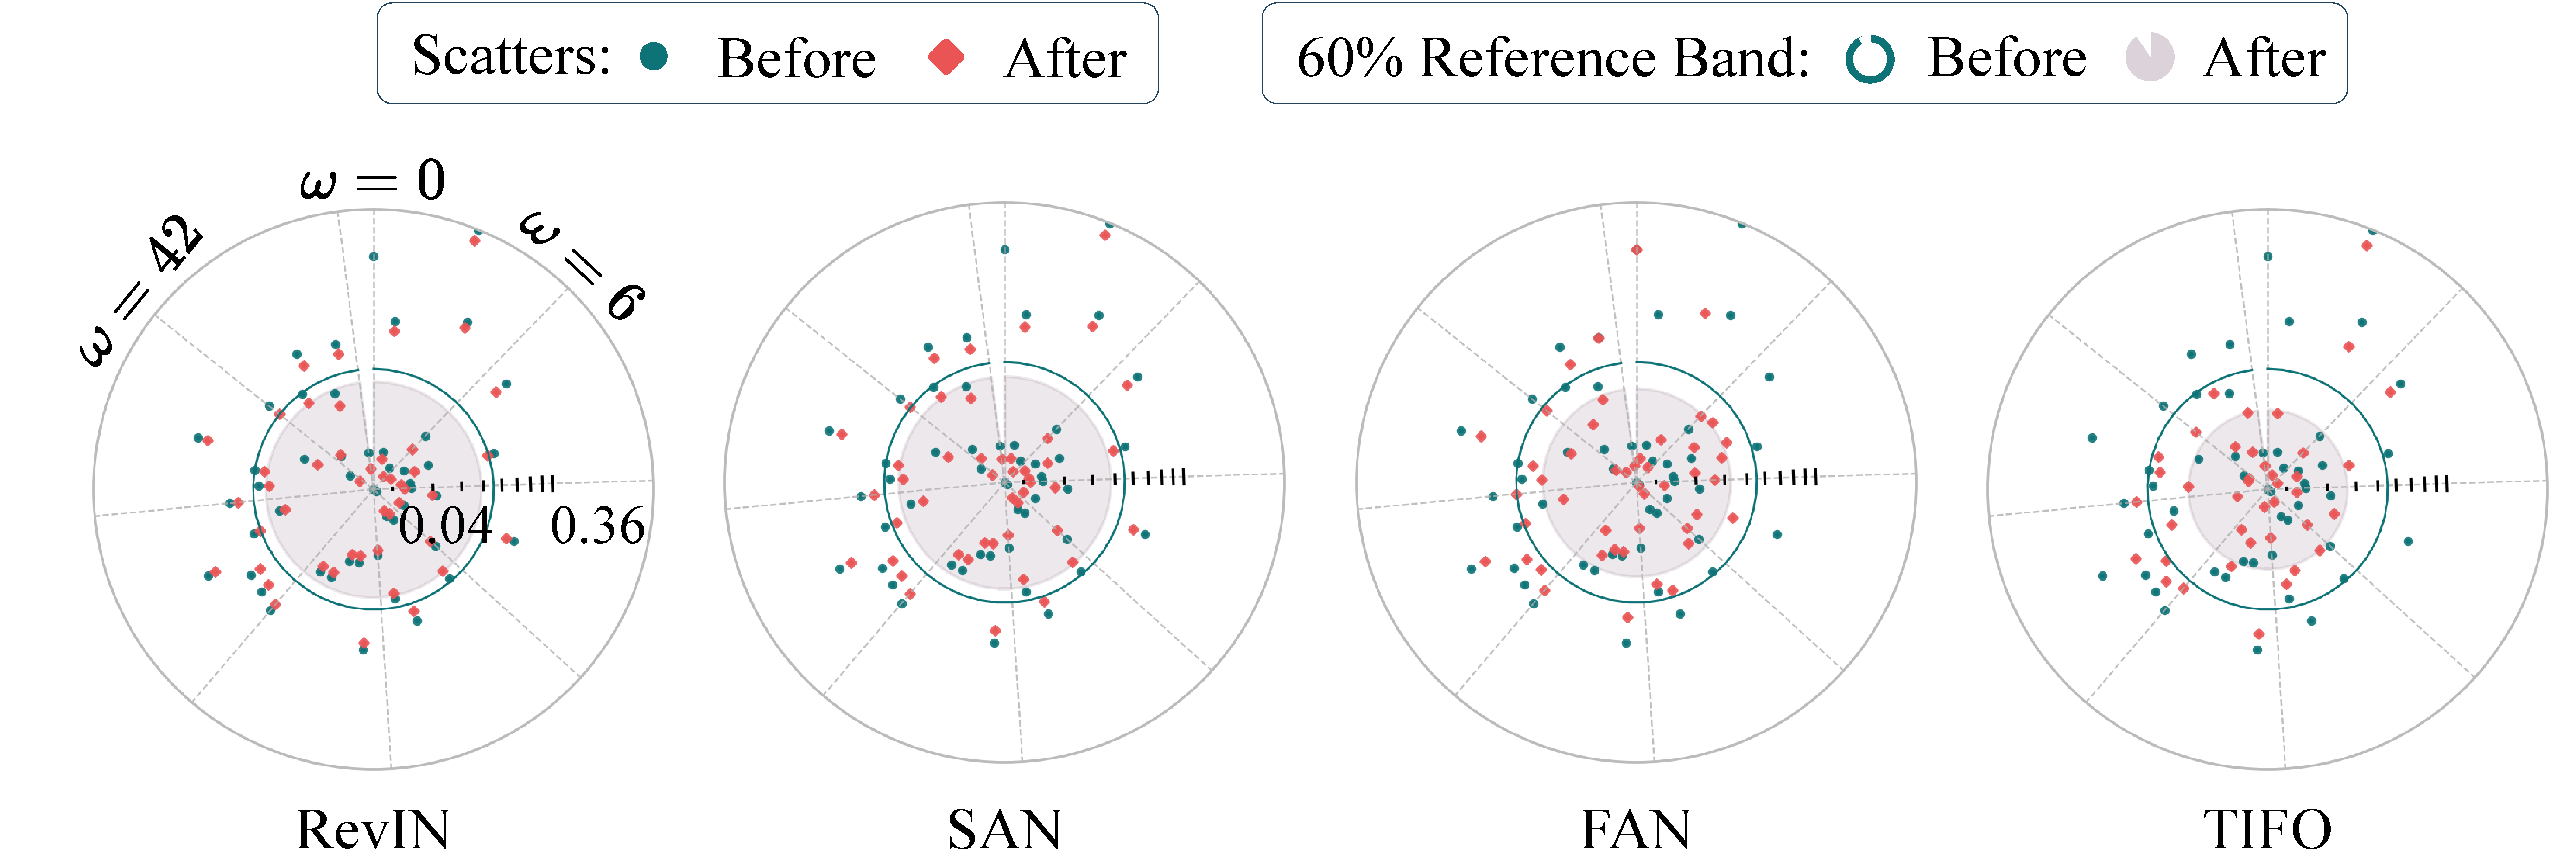
\includegraphics[width=\linewidth]{pics/app_result_2.pdf}
    \caption{
     More results on train-test distance compactness: 
     This figure shows another visualization of the JSD$^{2}$ amplitudes distribution distance between the train and test datasets on the electricity data (on a different channel). 
     Each scatter point represents one frequency component. 
     A smaller radius indicates a smaller distributional gap.  
     Green and red colors represent the results before and after applying the learning method, respectively.
     }
    \label{fig:shift_radar}
  \end{minipage} 

  % \vspace{1em}

  % \begin{minipage}{\linewidth}
  %   \centering
  %   \captionsetup{type=table}
  %   \caption{Frequency‑domain distribution distance between the train and test set.  
  %   Both the JSD$^{2}$ $(\downarrow)$ and the KS statistic $(\downarrow)$ are computed on amplitudes; bold marks the best per row.}
  %   \label{tab:freq_dist_flat}
  %   \resizebox{\textwidth}{!}{%
  %     \begin{tabular}{l
  %                     cc  % Raw
  %                     cc  % Z-score
  %                     cc  % FAN
  %                     cc  % SAN
  %                     cc} % TIFO
  %       \toprule
  %       Dataset 
  %         & \multicolumn{2}{c}{Before} 
  %         & \multicolumn{2}{c}{ReVIN} 
  %         & \multicolumn{2}{c}{FAN} 
  %         & \multicolumn{2}{c}{SAN} 
  %         & \multicolumn{2}{c}{\method} \\
  %       \cmidrule(lr){2-3} \cmidrule(lr){4-5} \cmidrule(lr){6-7} \cmidrule(lr){8-9} \cmidrule(lr){10-11}
  %         & JSD\textsuperscript{2} & KS 
  %         & JSD\textsuperscript{2} & KS 
  %         & JSD\textsuperscript{2} & KS 
  %         & JSD\textsuperscript{2} & KS 
  %         & JSD\textsuperscript{2} & KS \\
  %       \midrule
  %       ETTh1       & 0.36367 & 0.35982 
  %                   & 0.08100 & 0.08937 
  %                   & 0.14759 & 0.27057 
  %                   & 0.04745 & 0.08389 
  %                   & \textbf{0.04353} & \textbf{0.07357} \\
  %       % ETTm1       & 0.11677 & 0.15640 
  %       %             & 0.01983 & 0.07793 
  %       %             & 0.04603 & 0.12044 
  %       %             & \textbf{0.01080} & \textbf{0.06470} 
  %       %             & 0.01620 & 0.07267 \\
  %       weather     & 0.11156 & 0.19926 
  %                   & 0.02175 & 0.09172 
  %                   & 0.05328 & 0.12149 
  %                   & 0.01739 & 0.09566 
  %                   & \textbf{0.01687} & \textbf{0.07934} \\
  %       ECL         & 0.14431 & 0.16804 
  %                   & 0.08060 & 0.11924 
  %                   & 0.10394 & 0.16537 
  %                   & 0.07740 & 0.11639 
  %                   & \textbf{0.04225} & \textbf{0.09581} \\
  %       \bottomrule
  %     \end{tabular}%
  %   }
  % \end{minipage}
\end{figure*}

\subsubsection{Fourier Basis Learning Evaluation}

% Appendix: Additional 3D Frequency‐Spectrum Visualizations

We include here further 3D views of the ground truth vs. predicted amplitude spectra, sampled from different time‐series examples and channels. 
The forecasting horizon is fixed to $720$.
For each plot, we pick a specific sample index and a specific channel, to show that our \method\ consistently helps the model recover spectral peaks across the dataset:

\begin{itemize}

  \item \textbf{Compute amplitudes.}  
    For each method tag (\texttt{Before}, \texttt{FAN}, \texttt{\method}), we load a 1D slice \texttt{data[\dots ,sample,channel]}, take the real FFT via \texttt{rfft}, then smooth with \texttt{gaussian\_filter1d} and clip to $[z_{\min},z_{\max}]$.

  \item \textbf{Frequency‐to‐axis mapping.}  
    We linearly map the frequency index range $[\!f_{\min},f_{\max}]$ to the extended Y‐axis interval, and map amplitude values into the Z‐axis range plus a constant offset (\texttt{Z\_OFFSET}).

  \item \textbf{True vs.\ predicted curves.}  
    We plot the smoothed true spectrum (in blue) and the predicted spectrum (in red) at a constant $x$-plane (\texttt{X\_PLANE}), using 3D line plots.


\end{itemize}


\begin{figure*}[H]
  \centering
  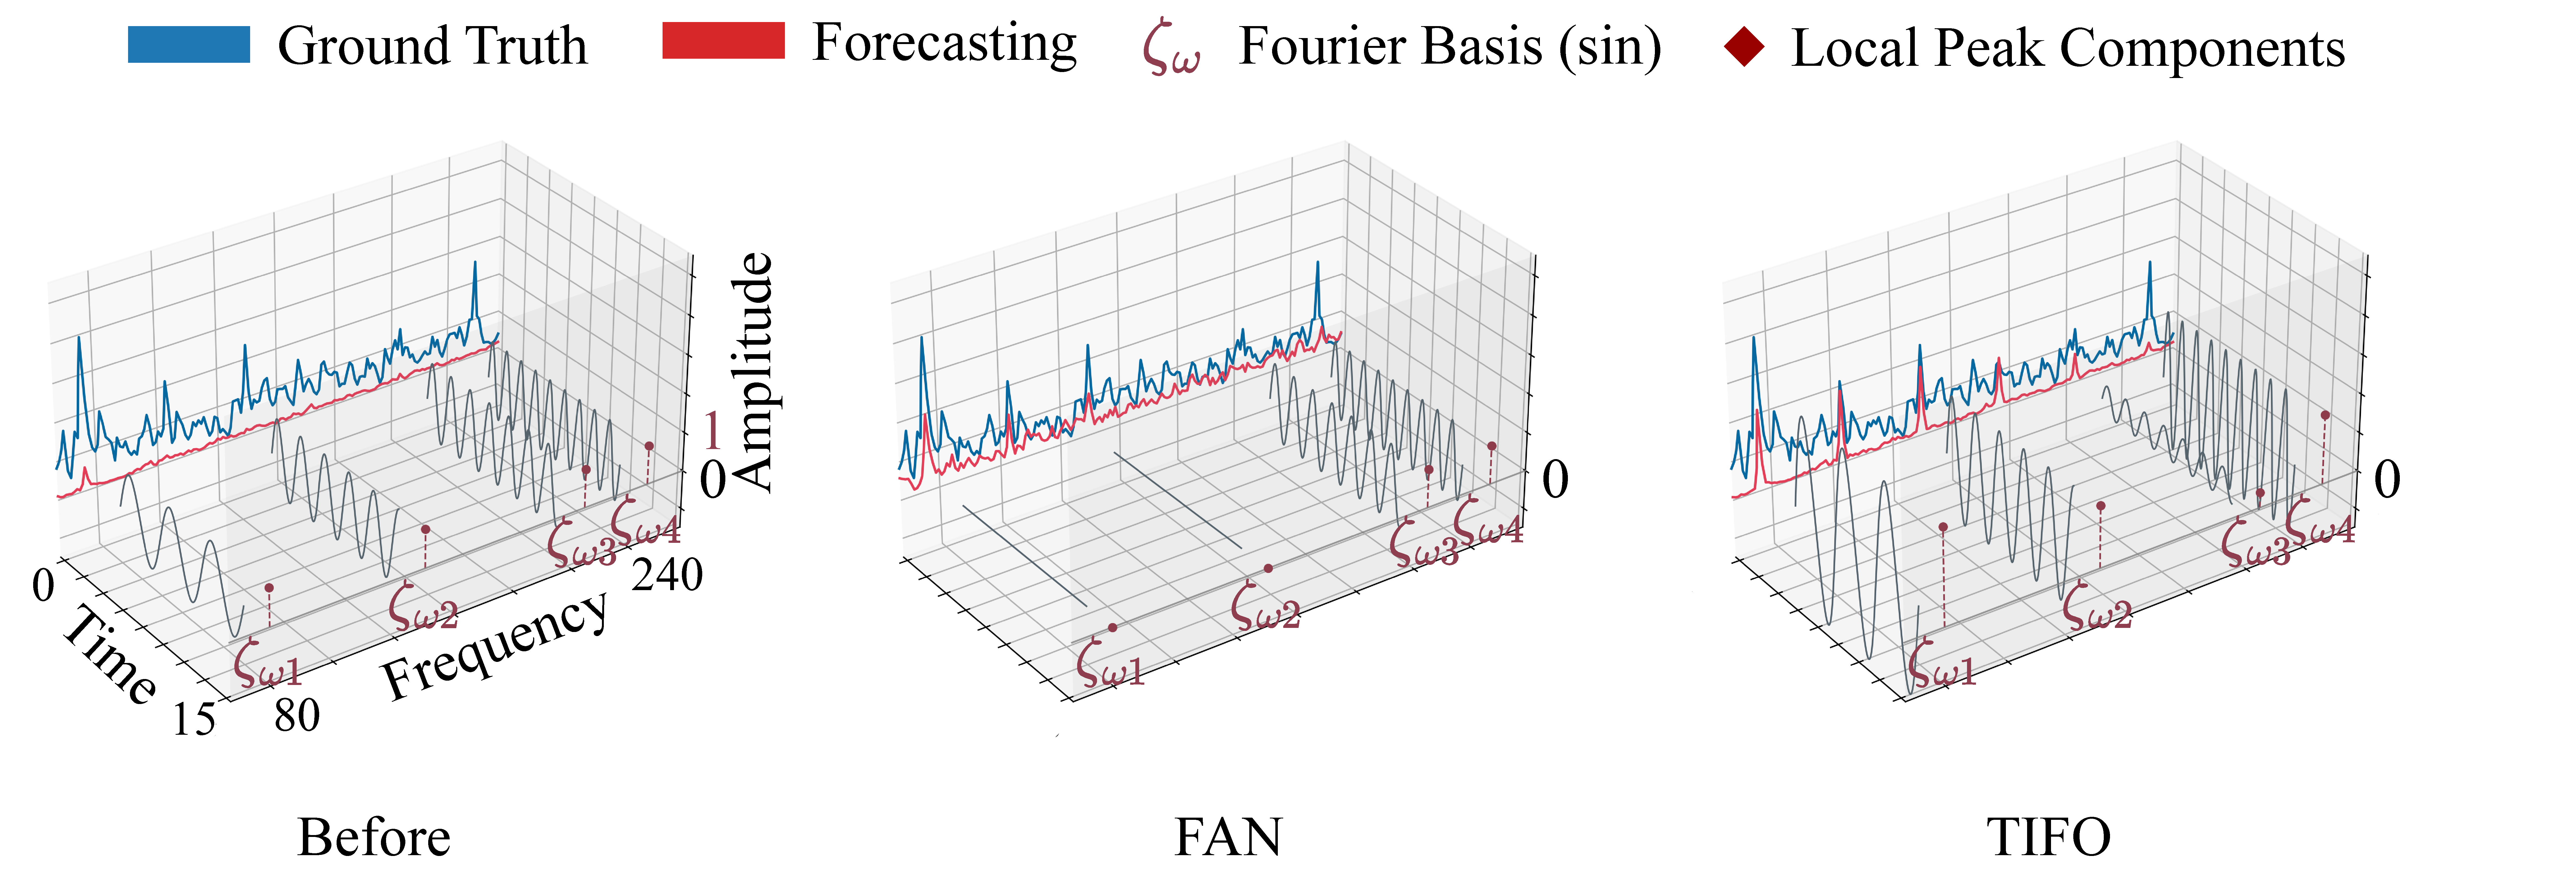
\includegraphics[width=\linewidth]{pics/app_freq_5.pdf}
  \caption{Frequency‐domain analysis of Fourier basis Learning. ETTh1 dataset, Channel \#1.
  }
  \label{fig:freq_results2}
\end{figure*}

\begin{figure*}[H]
  \centering
  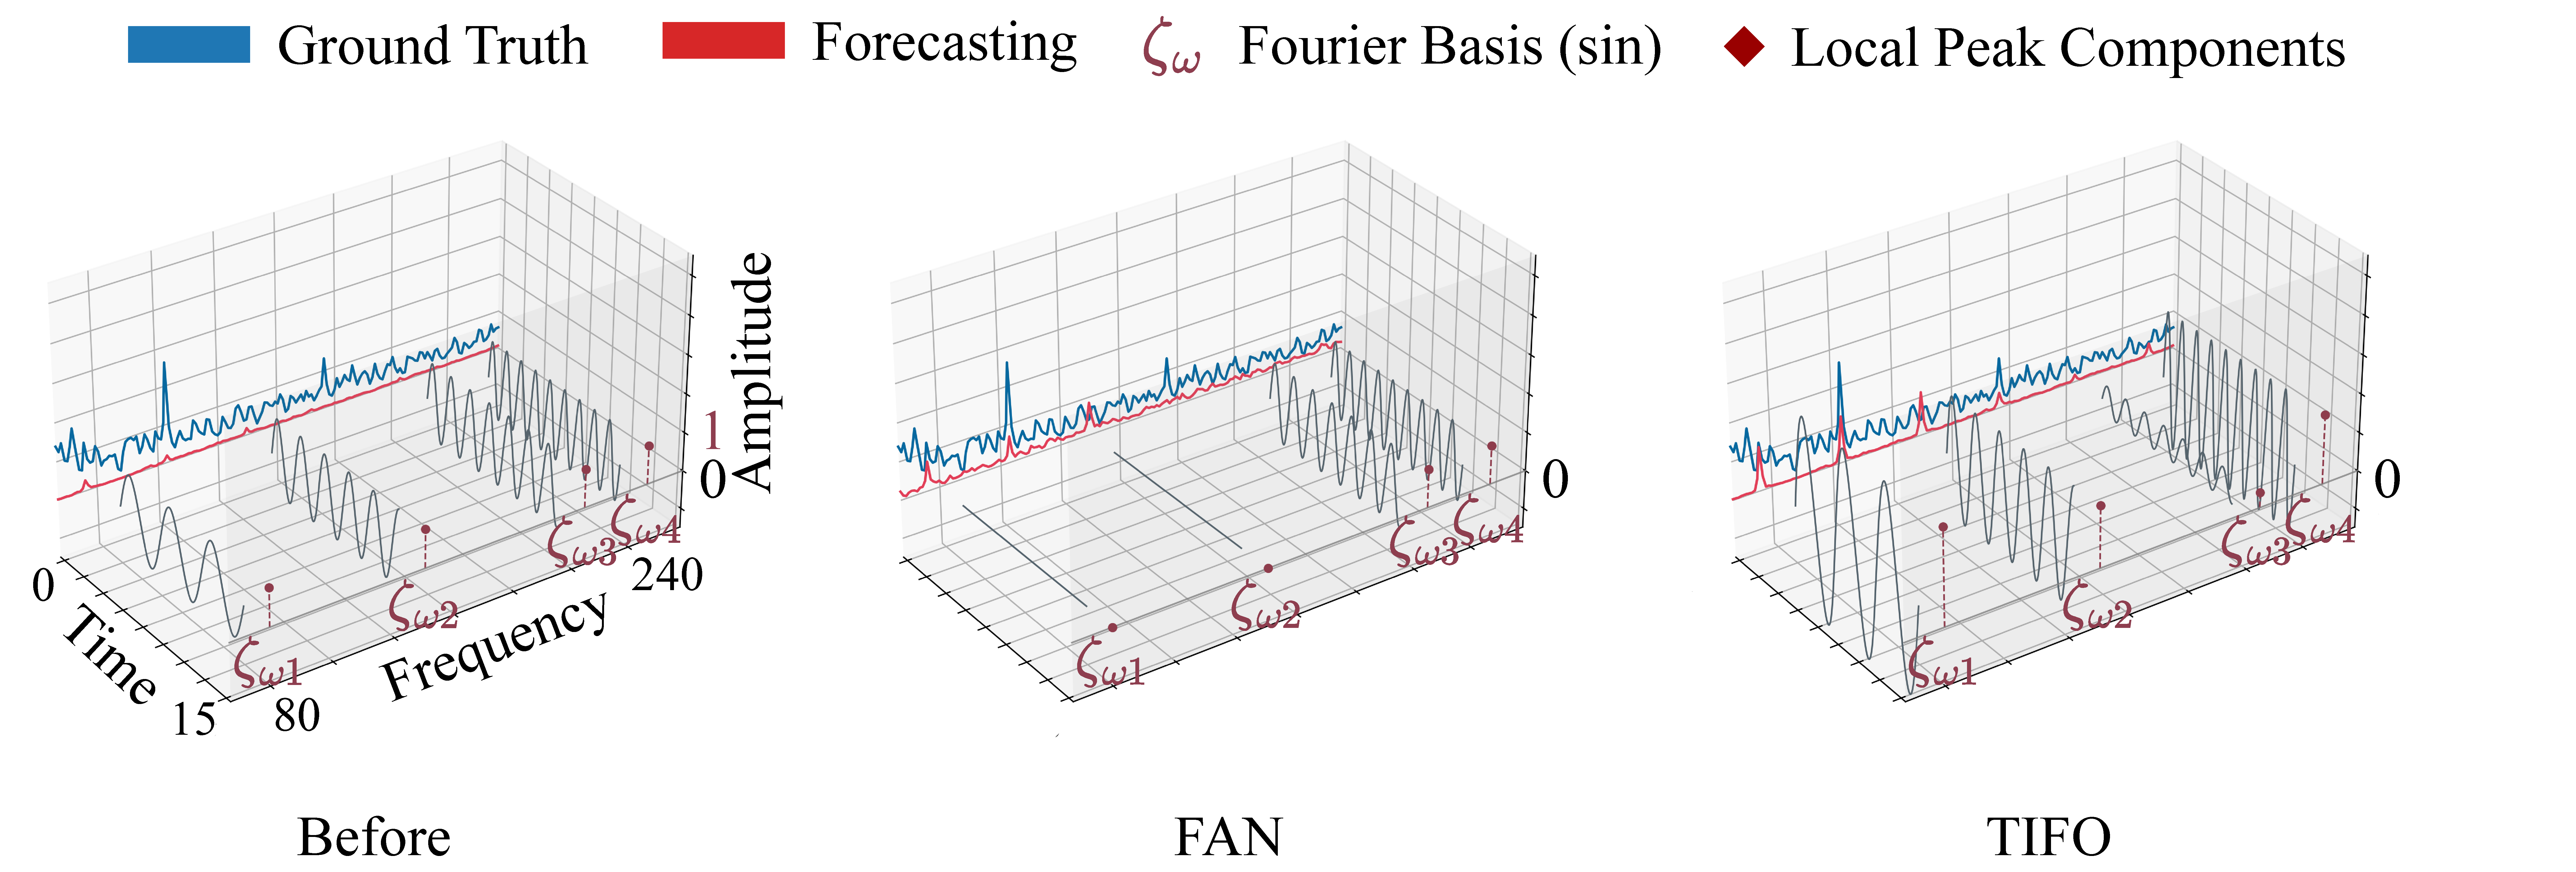
\includegraphics[width=\linewidth]{pics/app_freq_4.pdf}
  \caption{Frequency‐domain analysis of Fourier basis Learning. ETTm1 dataset, Channel \#2.
  }
  \label{fig:freq_results2}
\end{figure*}

\begin{figure*}[H]
  \centering
  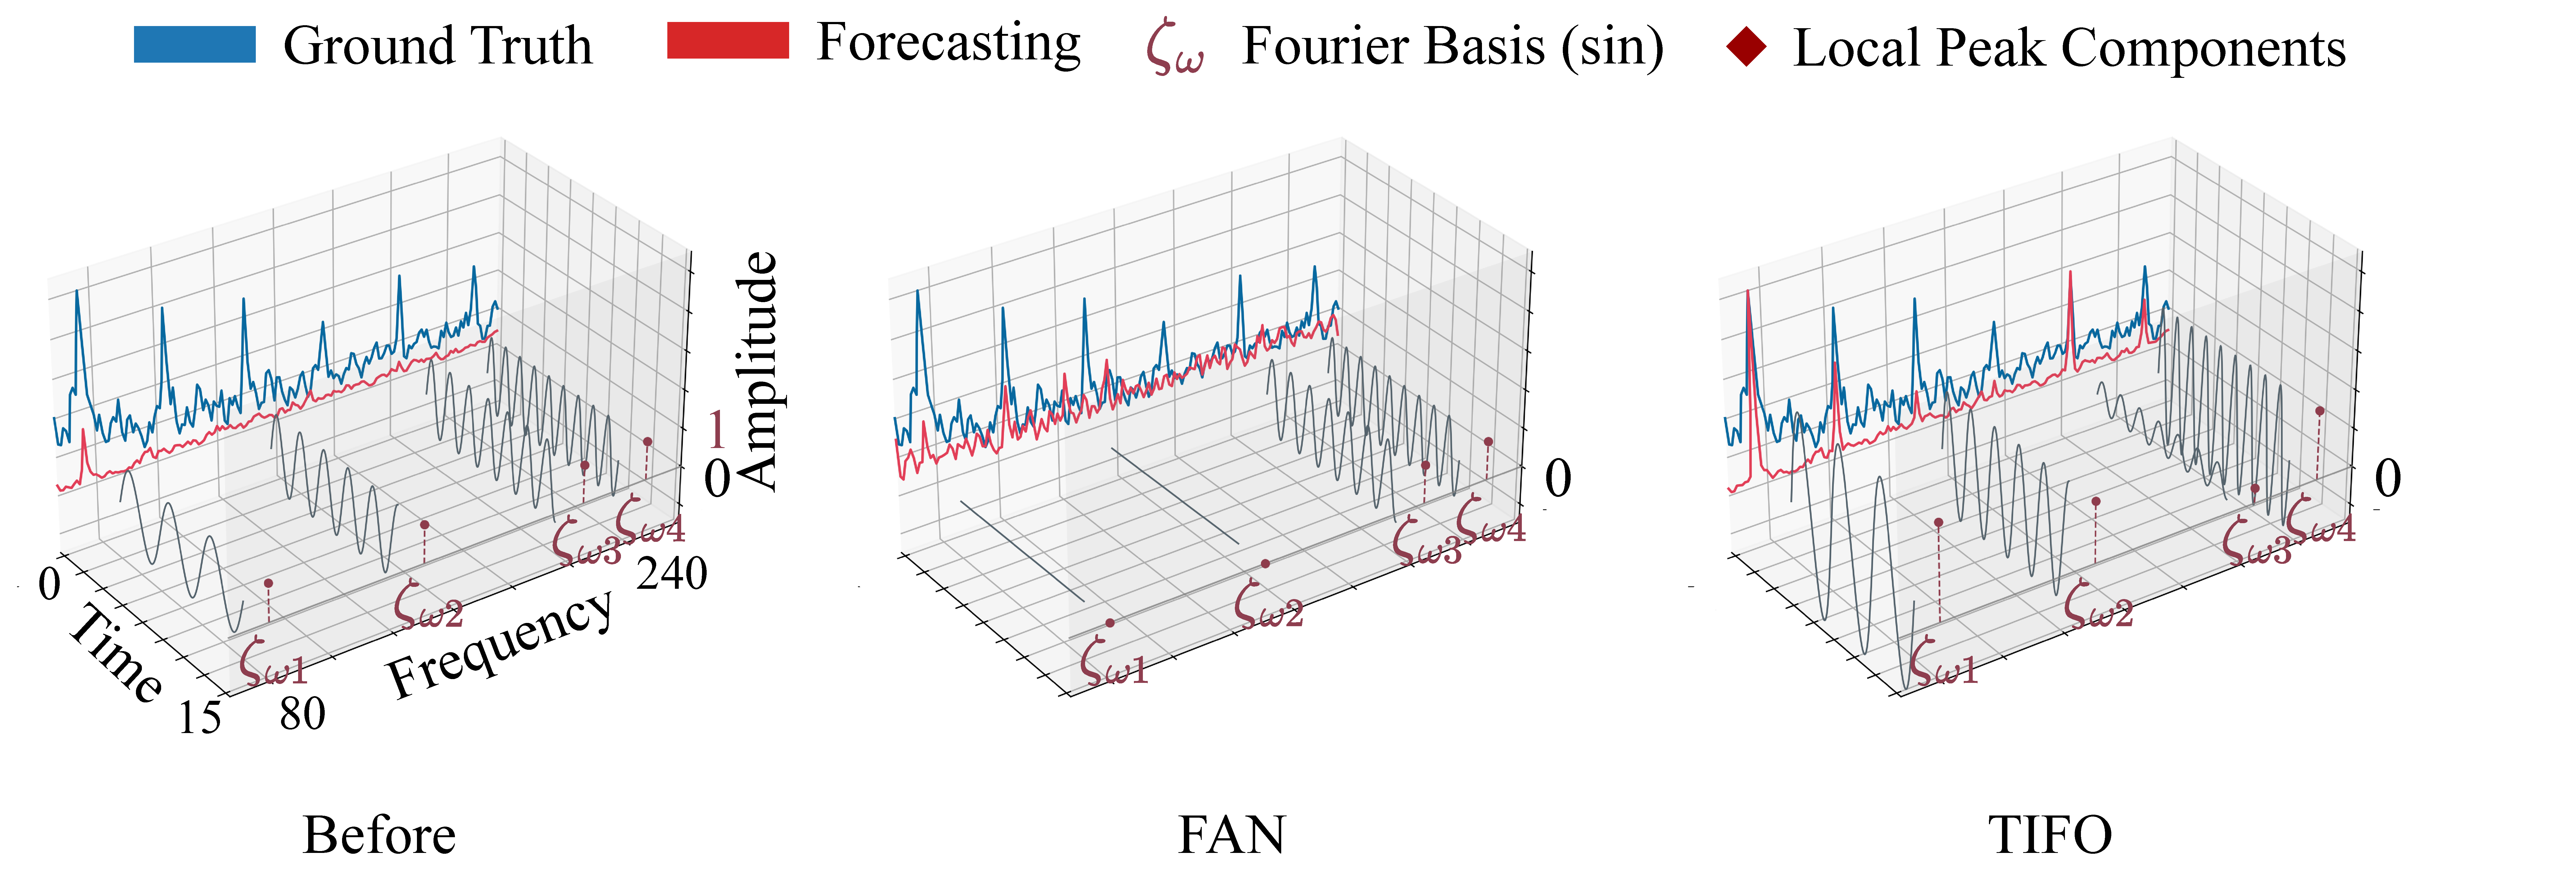
\includegraphics[width=\linewidth]{pics/app_freq_3.pdf}
  \caption{Frequency‐domain analysis of Fourier basis Learning. Traffic dataset, Channel \#237.
  }
  \label{fig:freq_results2}
\end{figure*}


\begin{figure*}[H]
  \centering
  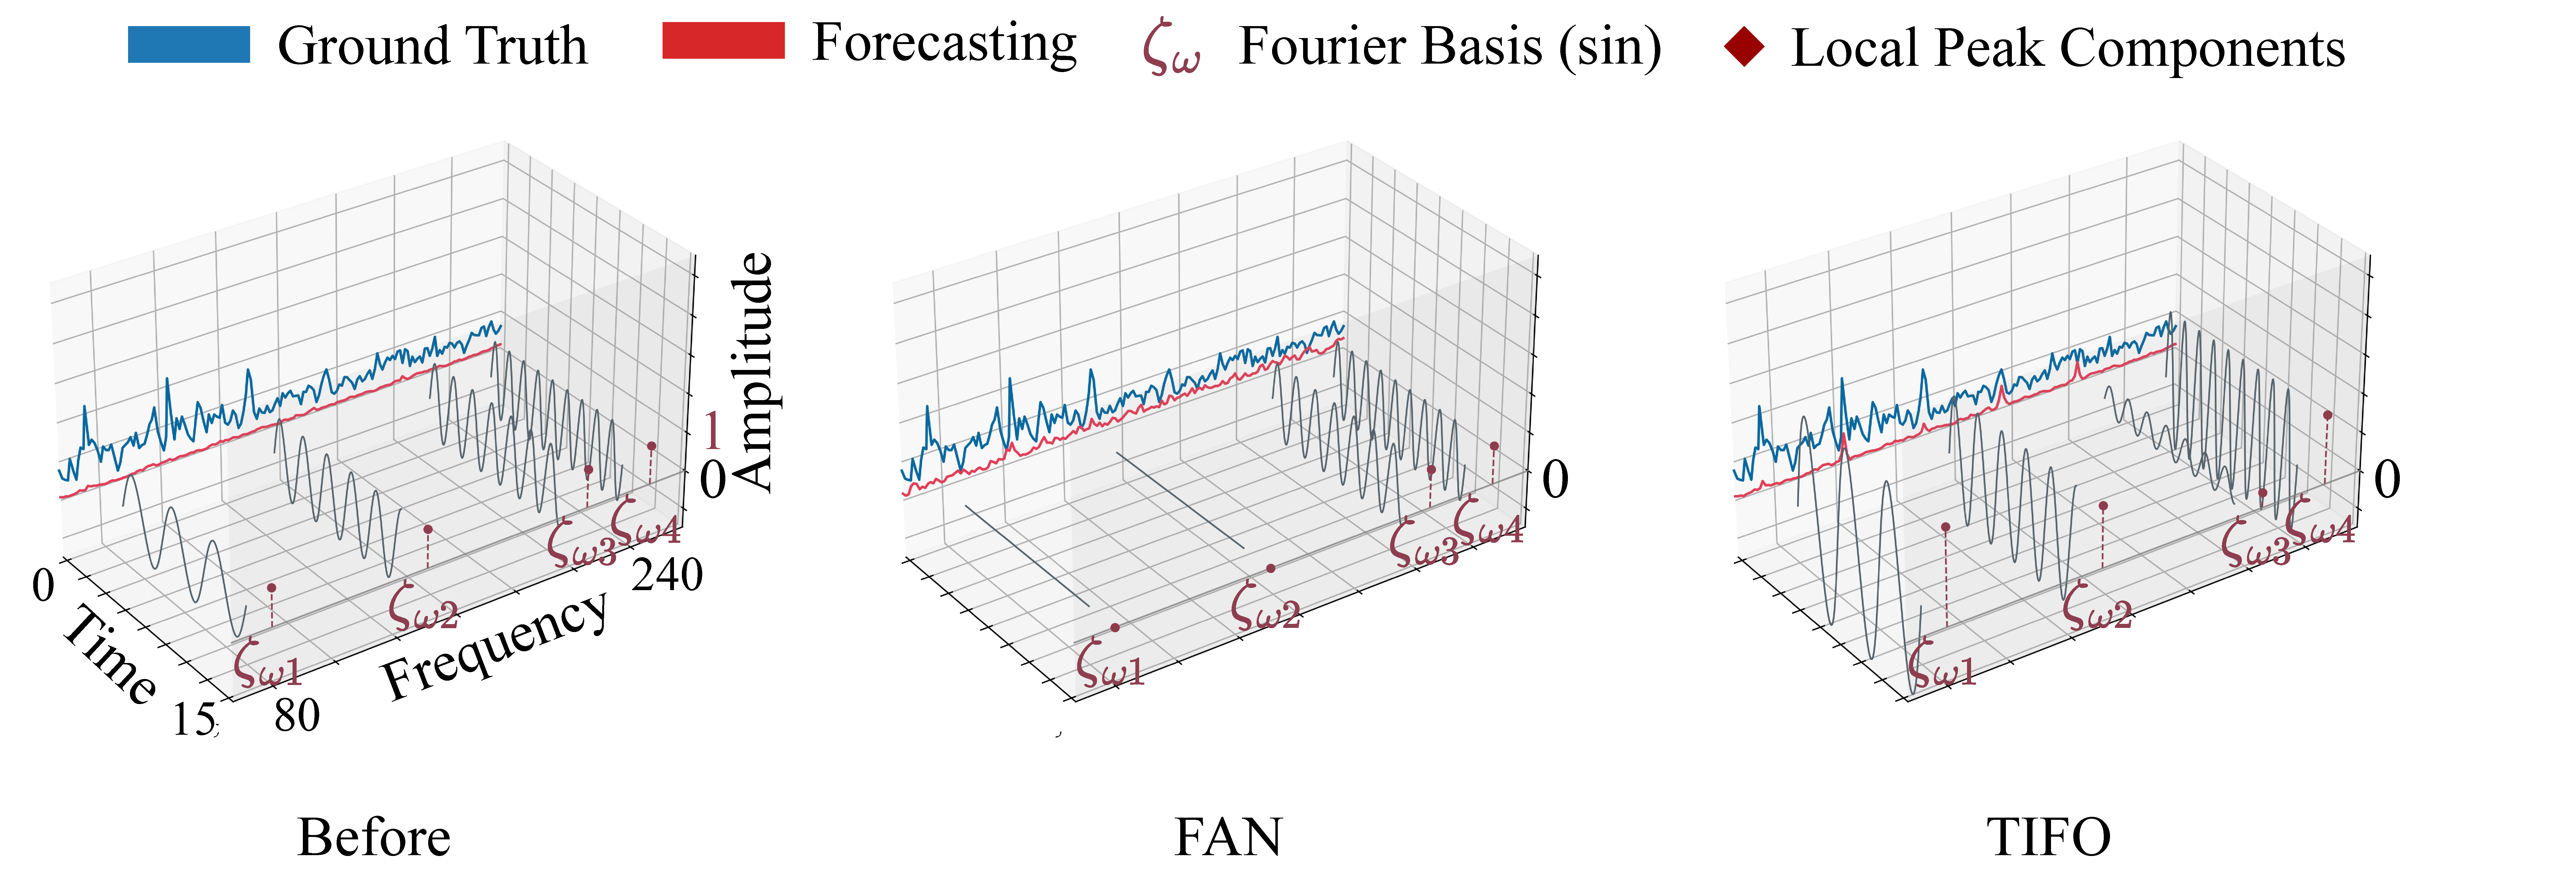
\includegraphics[width=\linewidth]{pics/app_freq_2.pdf}
  \caption{Frequency‐domain analysis of Fourier basis Learning. ETTh1 dataset, Channel \#6.
  }
  \label{fig:freq_results2}
\end{figure*}


\begin{figure*}[H]
  \centering
  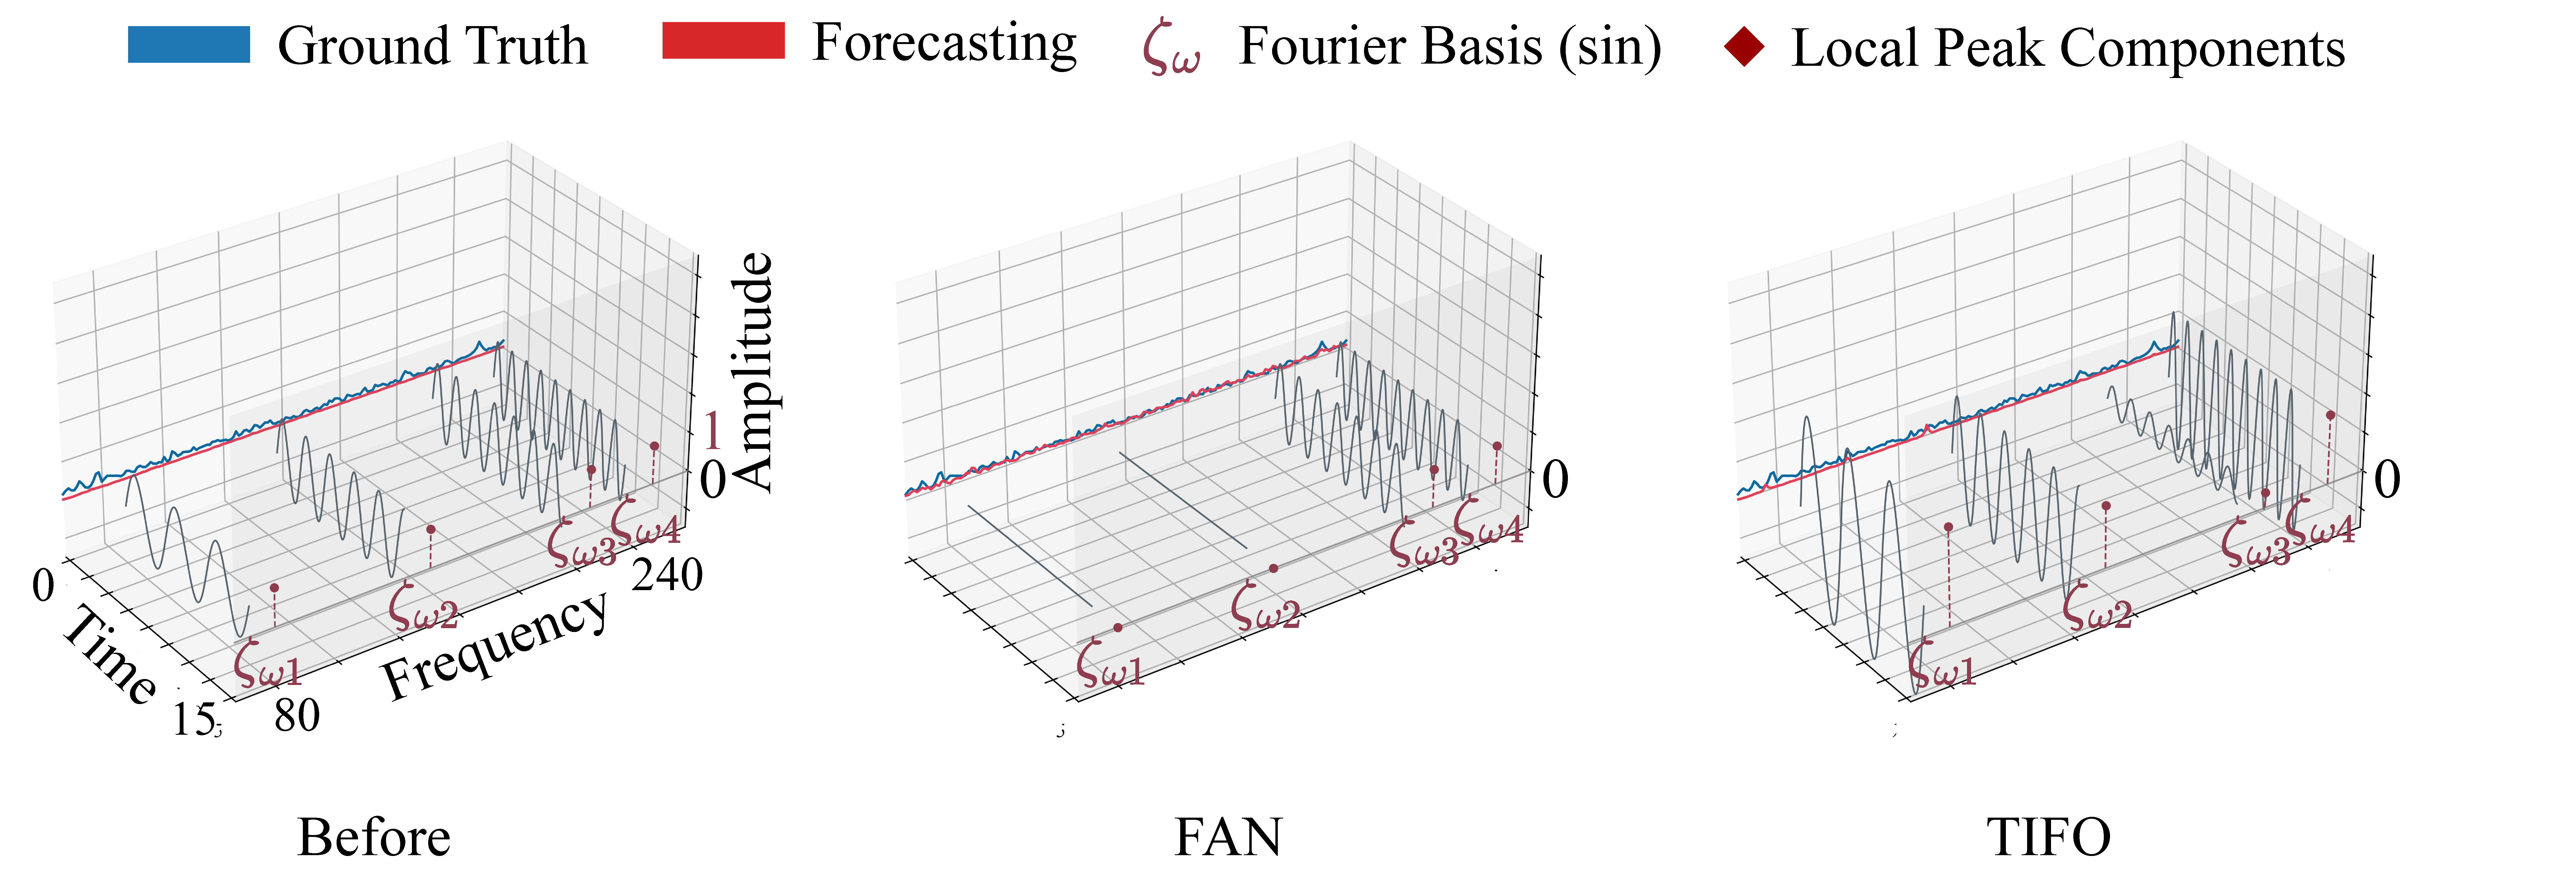
\includegraphics[width=\linewidth]{pics/app_freq_1.pdf}
  \caption{Frequency‐domain analysis of Fourier basis Learning. Weather dataset, Channel \#7. 
  }
  \label{fig:freq_results2}
\end{figure*}

\subsection{Running Time}
\label{app:running_time}


Table \ref{tab:time_comparison_transposed} presents the running time comprehensive results of our paper. 
This table includes the prediction accuracy outcomes on the [Electricity, ETTh1, ETTh2, ETTm1, ETTm2, Traffic, Weather] dataset, utilizing the [DLinear, PatchTST] as the backbone model. 
We compare our method against SAN across forecasting horizons $H \in \{96, 720 \}$. 

\begin{table*}[H]
\centering
\caption{Running time comparison with forecasting lengths $ H \in \{96, 720\}$ for all datasets and fixed input sequence length $L = 96$. The \textbf{best} results are highlighted.}
\label{tab:time_comparison_transposed}
\resizebox{\textwidth}{!}{
\begin{tabular}{c|*{7}{cc}}
\toprule
Model & \multicolumn{2}{c}{Electricity} & \multicolumn{2}{c}{ETTh1} & \multicolumn{2}{c}{ETTh2} & \multicolumn{2}{c}{ETTm1} & \multicolumn{2}{c}{ETTm2} & \multicolumn{2}{c}{Traffic} & \multicolumn{2}{c}{Weather} \\
\cmidrule(lr){2-3} \cmidrule(lr){4-5} \cmidrule(lr){6-7} \cmidrule(lr){8-9} \cmidrule(lr){10-11} \cmidrule(lr){12-13} \cmidrule(lr){14-15}
H & 96 & 720 & 96 & 720 & 96 & 720 & 96 & 720 & 96 & 720 & 96 & 720 & 96 & 720 \\
\midrule
\multicolumn{15}{c}{\textbf{DLinear \citep{DLinear}}} \\
\midrule
+ \method  
& \textbf{16.718} & \textbf{27.545} & \textbf{3.004 }& \textbf{3.082 }& \textbf{2.820 }& \textbf{3.222 }& \textbf{13.456} & \textbf{13.124} & \textbf{11.839} & \textbf{12.949} & \textbf{23.217} & \textbf{43.413} & \textbf{13.970} & \textbf{16.536} 
\\
+ SAN   
& 19.159 & 34.914 & 8.688 & 8.054 & 8.373 & 7.811 & 36.706 & 36.564 & 36.620 & 36.550 & 31.378 & 54.518 & 37.739 & 40.731 
\\
IMP(\%)   
& \textbf{12.8\%} & \textbf{21.1\%} & \textbf{65.5\%} & \textbf{60.5\%} & \textbf{66.6\%} & \textbf{58.3\%} & \textbf{63.1\%} & \textbf{64.2\%} & \textbf{67.8\%} & \textbf{64.3\%} & \textbf{26.0\%} & \textbf{20.3\%} & \textbf{63.0\%} & \textbf{59.9\%} \\
\midrule
\multicolumn{15}{c}{\textbf{PatchTST \citep{PatchTST}}} \\
\midrule
+ \method   
& \textbf{99.104} & \textbf{103.78}1 & \textbf{7.952 }& \textbf{8.215 }& \textbf{14.687} & \textbf{14.122} & \textbf{54.526} & \textbf{28.944} & \textbf{59.406} & \textbf{26.233} & \textbf{209.00}6 & \textbf{215.71}8 & \textbf{69.107} & \textbf{49.628} 
\\
+ SAN  
& 313.697 & 322.083 & 16.226 & 15.309 & 16.078 & 14.998 & 63.686 & 65.839 & 65.978 & 66.798 & 550.026 & 557.730 & 81.973 & 81.462 
\\
IMP(\%) 
& \textbf{68.4\%} & \textbf{67.7\%} & \textbf{51.6\%} & \textbf{46.2\%} & \textbf{8.00\%} & \textbf{5.20\%} & \textbf{14.3\%} & \textbf{56.0\%} & \textbf{10.0\%} & \textbf{60.7\%} & \textbf{61.6\%} & \textbf{61.2\%} & \textbf{15.9\%} & \textbf{39.8\%} 
\\
\bottomrule
\end{tabular}
}
\end{table*}

\subsection{More Experiments}

We have added several new experiments here:

(1) \textbf{Window function and FFT resolution.}
On ETTh1 with iTransformer, we study the sensitivity of TIFO to the choice of window function and frequency resolution under the original single global DFT/IDFT setting (no overlap).
We compare rectangular vs.\ Hann windows and $K=48$ vs.\ $K=96$ frequency bins. 
\reviewhighlight{The results (Table~X) show that using the full spectrum with a rectangular window (rect\_K96) gives the best performance with small variance across runs, and changing the window or $K$ within a reasonable range does not break the gains of TIFO. We therefore keep the simple global rectangular window with $K=96$ as the default.}

\begin{table}[t]
\centering
\caption{Ablation on window function and FFT resolution on ETTh1 with iTransformer. The \textbf{best} results are highlighted.}
\label{tab:win_fft}
\resizebox{\linewidth}{!}{
\begin{tabular}{l|*{3}{cc}|cc}
\toprule
\multirow{2}{*}{Setting}
& \multicolumn{2}{c}{Run 0}
& \multicolumn{2}{c}{Run 1}
& \multicolumn{2}{c}{Run 2}
& \multicolumn{2}{c}{Average} \\
\cmidrule(lr){2-3}\cmidrule(lr){4-5}\cmidrule(lr){6-7}\cmidrule(lr){8-9}
& MSE & MAE & MSE & MAE & MSE & MAE & MSE & MAE \\
\midrule
rect\_K48  & 0.4250 & 0.4420 & 0.4020 & 0.4180 & 0.4050 & 0.4210 & 0.4107          & 0.4270          \\
rect\_K96  & 0.3902 & 0.4068 & 0.3939 & 0.4105 & 0.3974 & 0.4140 & \textbf{0.3938} & \textbf{0.4104} \\
hann\_K48  & 0.4130 & 0.4260 & 0.4100 & 0.4240 & 0.4120 & 0.4250 & 0.4117          & 0.4250          \\
hann\_K96  & 0.4110 & 0.4240 & 0.4090 & 0.4230 & 0.4130 & 0.4260 & 0.4110          & 0.4243          \\
\bottomrule
\end{tabular}
}
\end{table}



(2) \textbf{Robustness--expressiveness trade-off by scaling TIFO weights.}
\reviewhighlight{To analyze whether suppressing non-stationary components harms the predictive upper bound, we train TIFO on ETTh1 with iTransformer and, at test time, multiply the learned frequency weights by a scalar $\alpha \in \{1.00, 0.75, 0.50, 0.25, 0.00\}$. Here $\alpha=0.00$ corresponds to removing TIFO. As shown in Table~Y, $\alpha=1.00$ and $\alpha=0.75$ achieve the best (and very similar) accuracy; performance starts to degrade at $\alpha=0.50$, and becomes clearly worse when $\alpha \le 0.25$ or when TIFO is disabled. This confirms a natural trade-off: fully using the learned TIFO weights improves robustness and accuracy, while aggressively shrinking them harms performance.}

\begin{table}[t]
\centering
\caption{Effect of scaling the learned TIFO weights at test time by $\alpha$ on ETTh1 with iTransformer. The \textbf{best} average performance is highlighted.}
\label{tab:alpha_scale}
\resizebox{\linewidth}{!}{
\begin{tabular}{c|*{4}{cc}|cc}
\toprule
\multirow{2}{*}{$\alpha$}
& \multicolumn{2}{c}{H = 96}
& \multicolumn{2}{c}{H = 192}
& \multicolumn{2}{c}{H = 336}
& \multicolumn{2}{c}{H = 720}
& \multicolumn{2}{c}{Average} \\
\cmidrule(lr){2-3}\cmidrule(lr){4-5}\cmidrule(lr){6-7}\cmidrule(lr){8-9}\cmidrule(lr){10-11}
& MSE & MAE & MSE & MAE & MSE & MAE & MSE & MAE & MSE & MAE \\
\midrule
0.00 & 0.4590 & 0.4740 & 0.5170 & 0.5100 & 0.5620 & 0.5330 & 0.5660 & 0.5520 & 0.5260      & 0.5172      \\
0.25 & 0.4540 & 0.4690 & 0.5120 & 0.5050 & 0.5570 & 0.5280 & 0.5610 & 0.5470 & 0.5210      & 0.5122      \\
0.50 & 0.4190 & 0.4340 & 0.4770 & 0.4700 & 0.5220 & 0.4930 & 0.5260 & 0.5120 & 0.4860      & 0.4773      \\
0.75 & 0.3900 & 0.4050 & 0.4440 & 0.4380 & 0.4940 & 0.4650 & 0.4990 & 0.4840 & 0.4567      & 0.4480      \\
1.00 & 0.3780 & 0.3930 & 0.4460 & 0.4390 & 0.4810 & 0.4520 & 0.4850 & 0.4710 & \textbf{0.4475} & \textbf{0.4388} \\
\bottomrule
\end{tabular}
}
\end{table}



(3) \textbf{Frequency decomposition strategies.}
\reviewhighlight{To address phase-distortion and boundary-effect concerns, we compare our original global FFT design with several STFT-style variants on ETTh1 + iTransformer: (i) \textit{Ori} (single global rectangular window, no overlap), (ii) \textit{hann\_50\_ola} (Hann, 50\% overlap, OLA), (iii) \textit{sqrt\_hann\_50\_wola} ($\sqrt{\text{Hann}}$, 50\% overlap, WOLA with COLA), and (iv) \textit{hann\_75\_ola} (Hann, 75\% overlap, OLA). Table~Z shows that Ori remains the best, the COLA-compliant WOLA variant is slightly worse, and Hann-based OLA variants significantly degrade accuracy. This indicates that, in our setting, the simple global FFT with finite-length periodicity assumption is sufficient, and additional windowing/overlap does not provide benefit.}

\begin{table}[h]
\centering
\caption{Comparison of reconstruction strategies (global DFT vs.\ OLA/WOLA) on ETTh1 with iTransformer. The \textbf{best} results are highlighted.}
\label{tab:recon_ola}
\resizebox{\linewidth}{!}{
\begin{tabular}{l|*{3}{cc}|cc}
\toprule
\multirow{2}{*}{Setting}
& \multicolumn{2}{c}{Run 0}
& \multicolumn{2}{c}{Run 1}
& \multicolumn{2}{c}{Run 2}
& \multicolumn{2}{c}{Average} \\
\cmidrule(lr){2-3}\cmidrule(lr){4-5}\cmidrule(lr){6-7}\cmidrule(lr){8-9}
& MSE & MAE & MSE & MAE & MSE & MAE & MSE & MAE \\
\midrule
Ori                  & 0.3902 & 0.4068 & 0.3939 & 0.4105 & 0.3974 & 0.4140 & \textbf{0.3938} & \textbf{0.4104} \\
hann\_50\_ola        & 0.5887 & 0.5148 & 0.5623 & 0.5053 & 0.5951 & 0.5152 & 0.5820          & 0.5118          \\
sqrt\_hann\_50\_wola & 0.3999 & 0.4135 & 0.3985 & 0.4133 & 0.4032 & 0.4175 & 0.4005          & 0.4148          \\
hann\_75\_ola        & 0.5872 & 0.5130 & 0.5627 & 0.5050 & 0.5944 & 0.5149 & 0.5814          & 0.5110          \\
\bottomrule
\end{tabular}
}
\end{table}


\begin{table}
\centering
\caption{Effect of online EMA refresh of frequency masks during inference on ETTh1 with iTransformer. The \textbf{best} results are highlighted.}
\label{tab:ema_refresh}
\resizebox{\linewidth}{!}{
\begin{tabular}{l|*{3}{cc}|cc}
\toprule
\multirow{2}{*}{Setting}
& \multicolumn{2}{c}{Run 0}
& \multicolumn{2}{c}{Run 1}
& \multicolumn{2}{c}{Run 2}
& \multicolumn{2}{c}{Average} \\
\cmidrule(lr){2-3}\cmidrule(lr){4-5}\cmidrule(lr){6-7}\cmidrule(lr){8-9}
& MSE & MAE & MSE & MAE & MSE & MAE & MSE & MAE \\
\midrule
no\_update & 0.3902 & 0.4068 & 0.3939 & 0.4105 & 0.3974 & 0.4140 & \reviewhighlight{\textbf{0.3938}} & \textbf{0.4104} \\
ema\_0.9   & 0.3916 & 0.4101 & 0.3930 & 0.4105 & 0.3952 & 0.4136 & \reviewhighlight{0.3932}          & 0.4114          \\
ema\_0.99  & 0.3903 & 0.4085 & 0.3938 & 0.4110 & 0.3966 & 0.4146 & 0.3936          & 0.4114          \\
\bottomrule
\end{tabular}
}
\end{table}


\begin{table}
\centering
\caption{Sensitivity to STFT hyperparameters (hop ratio and zero-padding) on ETTh1 with iTransformer. The \textbf{best} results are highlighted.}
\label{tab:hop_zpad}
\resizebox{\linewidth}{!}{
\begin{tabular}{l|*{3}{cc}|cc}
\toprule
\multirow{2}{*}{Setting}
& \multicolumn{2}{c}{Run 0}
& \multicolumn{2}{c}{Run 1}
& \multicolumn{2}{c}{Run 2}
& \multicolumn{2}{c}{Average} \\
\cmidrule(lr){2-3}\cmidrule(lr){4-5}\cmidrule(lr){6-7}\cmidrule(lr){8-9}
& MSE & MAE & MSE & MAE & MSE & MAE & MSE & MAE \\
\midrule
hop0.125\_zpad0.0 & 0.3950 & 0.4100 & 0.3980 & 0.4130 & 0.3990 & 0.4140 & 0.3973          & 0.4123          \\
hop0.125\_zpad0.5 & 0.3920 & 0.4070 & 0.3940 & 0.4090 & 0.3950 & 0.4100 & \textbf{0.3937} & \textbf{0.4087} \\
hop0.125\_zpad1.0 & 0.3930 & 0.4080 & 0.3950 & 0.4100 & 0.3960 & 0.4110 & 0.3947          & 0.4097          \\
hop0.25\_zpad0.0  & 0.3970 & 0.4120 & 0.4000 & 0.4150 & 0.4020 & 0.4170 & 0.3997          & 0.4147          \\
hop0.25\_zpad0.5  & 0.3950 & 0.4100 & 0.3970 & 0.4120 & 0.3980 & 0.4130 & 0.3967          & 0.4117          \\
hop0.25\_zpad1.0  & 0.3940 & 0.4090 & 0.3960 & 0.4110 & 0.3970 & 0.4120 & 0.3957          & 0.4107          \\
\bottomrule
\end{tabular}
}
\end{table}

(4) \textbf{Online EMA refresh of stability scores under drift.}
\reviewhighlight{We further test whether TIFO requires online updates of the stability-based weights in the presence of distribution drift. During inference on ETTh1 + iTransformer, we re-estimate batch-wise frequency statistics and update the global mask via exponential moving average with three settings: no update (no\_update), EMA with decay $0.9$, and EMA with decay $0.99$. The results (Table~W) show that all three settings yield almost identical MSE/MAE, and the small differences are well within run-to-run randomness; EMA($0.9$) gives a marginally smaller MSE. This suggests that dataset-level statistics estimated on the training set are already robust, and TIFO does not rely on frequent online re-estimation.}


(5) \textbf{Sensitivity to STFT hyperparameters (hop size and zero-padding).}
\reviewhighlight{Complementary to the global FFT analysis, we also conduct an STFT-style ablation on ETTh1 + iTransformer, varying hop ratio $\in \{0.125, 0.25\}$ and zero-padding ratio $\in \{0, 0.5, 1.0\}$. The results (Table~V) show that moderate zero-padding ($0.5$) yields consistent small gains across hop sizes, while further increasing zero-padding to $1.0$ brings negligible improvement. A smaller hop (larger overlap) is slightly better overall, but the effect is modest. Together with the previous experiments, this indicates that TIFO is reasonably robust to FFT-related hyperparameters and that sophisticated STFT configurations are not necessary for the gains reported in the main paper.}


% \section{LLM Usage Statement}
% We used large language models (LLMs) solely for writing support, including grammar correction, sentence refinement, and clarity improvements. All conceptual contributions, algorithm design, code development, experiments, and analyses were conducted entirely by the authors.


% \begin{table}[H]
%   \centering
%   \caption{Ablation study (mean $\pm$ std MAE↓). Bold marks the best per column.}
%   \label{tab:ablation}
%   \setlength{\tabcolsep}{3.5pt}
%   \renewcommand{\arraystretch}{1.15}
%   % ---- begin resizebox ----
%   \resizebox{\linewidth}{!}{%
%     \small
%     \begin{tabular}{
%       ll
%       S[table-format=1.3(2)]
%       S[table-format=1.3(2)]
%       S[table-format=1.3(2)]
%       S[table-format=1.3(2)]
%       S[table-format=1.3(2)]
%       S[table-format=1.3(2)]
%     }
%     \toprule
%     \multicolumn{2}{c}{Variant} &
%     \multicolumn{6}{c}{Dataset / Horizon} \\
%     \cmidrule(lr){3-8}
%     & & {ETTh1‑96} & {ETTh1‑720} & {ETTm1‑96} & {ETTm1‑720} & {Weather‑96} & {Weather‑720} \\
%     \midrule
%     Ours      & DLinear      & \bf 0.371 \pm 0.032 & \bf 0.428 \pm 0.039 & \bf 0.299 \pm 0.021 & \bf 0.425 \pm 0.032 & \bf 0.162 \pm 0.045 & \bf 0.325 \pm 0.041 \\
%               & iTransformer & \bf 0.389 \pm 0.023 & \bf 0.496 \pm 0.034 & \bf 0.330 \pm 0.035 & \bf 0.475 \pm 0.043 & \bf 0.162 \pm 0.044 & \bf 0.340 \pm 0.036 \\
%     Low‑pass  & DLinear      & 0.379 \pm 0.025 & 0.435 \pm 0.036 & 0.305 \pm 0.022 & 0.431 \pm 0.031 & 0.170 \pm 0.089 & 0.337 \pm 0.024 \\
%               & iTransformer & 0.401 \pm 0.017 & 0.502 \pm 0.029 & 0.335 \pm 0.033 & 0.483 \pm 0.047 & 0.171 \pm 0.055 & 0.356 \pm 0.039 \\
%     Random    & DLinear      & 0.393 \pm 0.066 & 0.440 \pm 0.087 & 0.308 \pm 0.053 & 0.429 \pm 0.079 & 0.171 \pm 0.102 & 0.345 \pm 0.065 \\
%               & iTransformer & 0.407 \pm 0.048 & 0.533 \pm 0.055 & 0.339 \pm 0.055 & 0.487 \pm 0.061 & 0.172 \pm 0.088 & 0.372 \pm 0.059 \\
%     \bottomrule
%     \end{tabular}%
%   }
% \end{table}




\end{document}
\endinput
%%
%% End of file `sample-sigconf.tex'.
